%\documentclass[12pt]{article}
\documentclass[12pt,twoside]{article}
\usepackage[utf8]{inputenc}

\raggedbottom

% HEADER and FOOTER
% http://www.sharelatex.com/learn/Headers_and_footers
\usepackage{fancyhdr}
\pagestyle{fancy}
\fancyhf{}
% header
\fancyhead[LE,RO]{\leftmark} %
\fancyhead[RE,LO]{\thepage}
% footer (ikke i bruk atm)
%\fancyfoot[CE,CO]{\leftmark}
%\fancyfoot[LE,RO]{\thepage}

\setlength{\headsep}{0.6in} % Mellomrom mellom header og body


%%%%%%%%%%RIKARD
\usepackage{courier}
\usepackage[T1]{fontenc}
\usepackage{ae,aecompl}
\usepackage{times}
\usepackage[font=small]{caption}
%%%%%%%%%%RIKARD

\usepackage{rotating}
\usepackage{tikz}


\usepackage{caption}
\usepackage{graphicx}
\usepackage{subcaption}
\usepackage{float}
\usepackage{hyperref}
\usepackage{multicol}
\usepackage[nottoc]{tocbibind}
\usepackage{supertabular}

\floatstyle{plaintop}
\restylefloat{table}
\usepackage{longtable}
\usepackage{morefloats}
\usepackage[titletoc]{appendix}
\usepackage{pdfpages}

\usepackage{adjustbox} % test
\usepackage{tabularx} % test
\usepackage{chngpage} % test
\usepackage{booktabs} % unødvendig

\usepackage[strict]{changepage}

\usepackage[acronym, toc, nonumberlist]{glossaries}
\makenoidxglossaries 
\newglossaryentry{EMR}
{
    name=EMR,
    description={Electronic Medical Record}
}

\newglossaryentry{PAS}
{
    name=PAS,
    description={Patient Administration System}
}

\newglossaryentry{HIS}
{
    name=HIS,
    description={Hospital Information Systems}
}

\newglossaryentry{DICOM}
{
    name=DICOM,
    description={A file format and network communications protocol that is used to transfer different medical information online}
}

\newglossaryentry{SSN}
{
    name=SSN,
    description={Social Security Number. Number used to uniquely identify individuals}
}

\newglossaryentry{aes}
{
    name=AES,
    description={Advanced Encryption Standard}
}

\newglossaryentry{GEHealthcare}
{
    name=GE Healthcare,
    description={GE Healthcare is a manufacturer of clinical grade devices and technology.}
}

\newglossaryentry{OUS}
{
    name=OUS,
    description={Oslo University Hospital}
}

\usepackage[british]{babel}
\usepackage[urldate=long]{biblatex}
\bibliography{bibliography.bib}

\usepackage{titlesec}
\setcounter{secnumdepth}{4}
\titleformat{\paragraph}{\normalfont\normalsize\bfseries}{\theparagraph}{1em}{}
\titlespacing*{\paragraph}{0pt}{3.25ex plus 1ex minus .2ex}{1.5ex plus .2ex}

% fjerner markering av lenker ved export av pdf
\hypersetup{%
    pdfborder = {0 0 0}
}

%Codeformat
\usepackage{listings}
\usepackage{color}

\definecolor{dkgreen}{rgb}{0,0.6,0}
\definecolor{gray}{rgb}{0.5,0.5,0.5}
\definecolor{mauve}{rgb}{0.58,0,0.82}
\definecolor{gray}{rgb}{0.4,0.4,0.4}
\definecolor{cyan}{rgb}{0.0,0.6,0.6}

\lstset{frame=single, framesep=8pt,
  language=Java,
  aboveskip=3mm,
  belowskip=3mm,
  showstringspaces=false,
  numbers=left,
  numberstyle=\footnotesize,
  stepnumber=1,
  numbersep=11pt, 
  captionpos=b,
  columns=flexible,
  basicstyle={\small\ttfamily},
  numberstyle=\tiny\color{gray},
  keywordstyle=\color{blue},
  commentstyle=\color{dkgreen},
  stringstyle=\color{mauve},
  breaklines=true,
  breakatwhitespace=true
  tabsize=3
}

%XML code
\lstdefinelanguage{XML}
{
  morestring=[b]",
  morestring=[s]{>}{<},
  morecomment=[s]{<?}{?>},
  stringstyle=\color{black},
  identifierstyle=\color{blue}
}

% Setter dybden på table of contents
\setcounter{tocdepth}{3} 

% For table cell padding
\usepackage{array}

%\addtolength{\topmargin}{-.4in} %top margin
%\addtolength{\textheight}{-.5in} %bot margin


\begin{document}

\begin{titlepage}
    \begin{center}
        \vspace*{1cm}
        
        \huge{Master Thesis}
        
        \vspace{1cm}
        \normalsize
        Exploring wireless ECG monitoring and the implementation of low energy sensors for clinical ambulatory patient monitoring.
        \vspace{1.5cm}
        
        \normalsize
        {Rikard Eide}
        
        \vfill
        
        
        \vspace{0.8cm}
        
        NTNU: Norwegian University of Science and Technology\\
        \today
        
    \end{center}
\end{titlepage}
\include{abstract}

\tableofcontents

\section{Project introduction}
\label{project_introduction}
% 1/3 rapporter har noe tekst her. Enn så lenge så prioriterer vi ikke det.


\subsection{Project goal}
The goal of this project is to develop software for a customer and document the process of the development. The group was issued the task of researching and developing an application aimed at the medical industry. This was to be a proof-of-concept application to shed light upon all the various aspects one has to consider while developing for the health sector. With a presumed, future smart device, running on the Android platform, the customer wanted an application that was able to connect wirelessly to existing hospital information systems in order to store ultrasound images and related data. This device is capable of receiving ultrasound images and video from a connected ultrasound probe over a common wired interface. The application would then be able to download relevant information about a patient, combine it with examination data (images and meta) and upload it to existing hospital information systems. Being an international company, the customer want this to work with different existing hospital information systems on an international scale.

\subsection{Customer}
The customer is the international consulting firm Capgemini. They are collaborating with GE Healthcare, a company providing medical technologies and services around the world \cite{gehealthcare}. GE Vingmed Ultrasound is a division of GE Healthcare based in Horten, Norway. They are the team behind the handheld ultrasound device Vscan (Figure \ref{vscandevice}). Vscan is an award-winning \cite{vscan_awards} portable ultrasound device used by doctors worldwide. GE Vingmed is looking to expand the functionality of this device, and this is the basis for the project.

\begin{figure}[H]
\centering
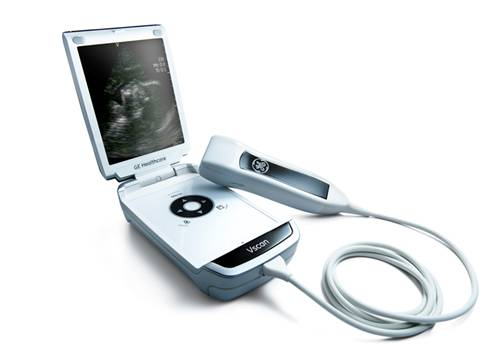
\includegraphics[scale=0.60]{img/vscan.jpg}
\caption{The Vscan Device}
\label{vscandevice}
\end{figure}

\subsection{Project scope}
The original intention of the customer was for us to deliver a system that worked on a global scale, meeting legal requirements in hundreds of countries, working across several different standards and protocols for exchanging medical information and communicating with several different existing hospital information systems. It did not take a lot of research to realize that this was a more than an ambitious goal \cite{metricFuckton}. Therefore, an agreement with the customer was made to reduce the scope of the project. Not even the Norwegian hospitals in the same region have agreed on a standard IT infrastructure, so we decided to focus on the largest institution in Norway, Oslo University Hospital (OUS), and the systems in use there.

This means researching and learning how the largest vendors of \emph{Patient Administration Systems} (PAS) and \emph{Electronic Medical Records} (EMR) work. Along with this we will look at future standards and solutions.

\subsection{Project constraints and resources}
Some of the constraints for this project are the limited documentation regarding software implementation of the EMRs and the systems that surrounds them, as well as the use of proprietary technology by many of the EMRs. This have made it hard for the group as developers to design and implement the functionality for communication with these systems, as well as testing the application against the systems it is designed for. 

To counter this issue, we have actively been trying to get in touch with people in the industry that might be able to help with understanding the necessary communication between the EMR clients and servers.   
\section{Project Planning}
A good amount of planning to make sure the group has been well organized were invested early in the project. In this section the planning phase will be presented. An evaluation of how this worked out over the course of the project can be found in chapter \ref{evaluation} Evaluation.

 
\subsection{Group organization}
The group has consisted of five Computer Science students, all finishing their third year at NTNU.

At an early stage in the project, the group decided to not assign strict areas of responsibility, apart from the Scrum-master position. The reason behind this is the nature of the project task. A lot of research needed to be done before getting a good overview of the task, and how extensive each part was. Giving narrow areas of responsibility therefore seemed unnecessary. However, a rough outline of main areas of responsibility were set. Below follows a brief presentation of each group member and their responsibilities.
\\

\noindent \textbf{Rikard Eide} \\
Scrum-master. Rikard has previously worked three years part time at a hospital. Based on this experience he was given the main responsibility with researching the industry. He has experience with Java, and is familiar with C\# and .Net.
\\

\noindent \textbf{Magnus Lund} \\
Magnus has experience with Java, \LaTeX\ and has worked on a couple of smaller Android projects. His main responsibility was managing the code- and application parts of the project.
\\

\noindent \textbf{Jens Kristian Espevik} \\
Jens Kristian's main responsibility, aside from coding, has been with group formalities, such as constructing meeting notes, weekly updates and report writing.
\\

\newpage

\noindent \textbf{Andreas Røyrvik} \\
Andreas has experience with server management and back-end development, and this has been his main responsibility.
\\

\noindent \textbf{Joakim Pettersen} \\
Joakim has experience with Java and Android. Joakim's main responsibility was testing.
\\


\subsection{Project management tools}
\label{project_management_tools}
To administrate the sprints and project organization in general, it was together with the customer, decided to use Confluence \cite{confluence} and JIRA Agile \cite{jira}. These are common tools in the industry which the group was recommended to use. The customer had access to both of these tools, and could follow the progress closely.

\subsubsection{Confluence}
Confluence is a team collaboration tool. Necessary diagrams and figures were developed with plugins found in the system. Other documentation, such as user manuals, technical descriptions and various tables were created, maintained and stored in Confluence. Confluence is used to ensure that the documentation is stored in such a way that it is easy to navigate and update if needed.

\subsubsection{JIRA Agile}
JIRA Agile is an issue tracker used to track, assign and report work tasks. JIRA helped the group visualize remaining tasks in each sprint as well as providing tools for generating progress reports based on task completion.


\subsection{Communication}
To communicate on a daily basis, the group used Google+'s Hangouts and Groups \cite{hangouts}. In addition to traditional real time text based chat, Google Hangouts offers video and voice chat. This turned out to be an useful feature when doing daily Scrum stand-ups on days where no in-person meetings were held.

To communicate with the customer and the supervisor, traditional email was used. In addition to communication over email, the group had bi-weekly meetings with the supervisor and customer.

\subsection{Work breakdown}
\label{workbreakdown}

The group did not receive any formal requirements from the customer. To get a better understanding of the customer's idea of the application built, frequent meetings were arranged in the beginning of the project period. To prepare for these customer meetings, the group had frequent internal meetings as well. In these meetings we discussed our initial impression of the application idea, and our thoughts about requirements. It was decided that each group member was to create several user stories, and present them to the group. A compilation of what we though would be the most relevant user stories were put together and presented to the customer.

The group also tried to identify what was the major work areas of the project, such as GUI implementation, image handling, user authentication etc. To help decide how extensive these tasks were, the group used Scrum poker cards to assign a weighted value to these areas of development.

This eventually lead to the creation of \emph{epics}. In agile development an epic is a compiled set of user stories describing a major product feature. The group then used the estimates to assign these epics to specific sprints, as seen in Figure \ref{fig:sprinter_oversikt}. Because we recognized this project would depend on research and information not yet obtained, traditional planning tools like Gantt and work-break-down charts were deemed ineffective. The group attempted to design the epics to be as independent of each other as possible, to allow for implementation of them in any order. The sprints were assigned ''code-names'', making it easier to distinguish between them. A discussion on how this process panned out during the project, can be found in section \ref{researchEval}.


\begin{figure}[H]
\centering
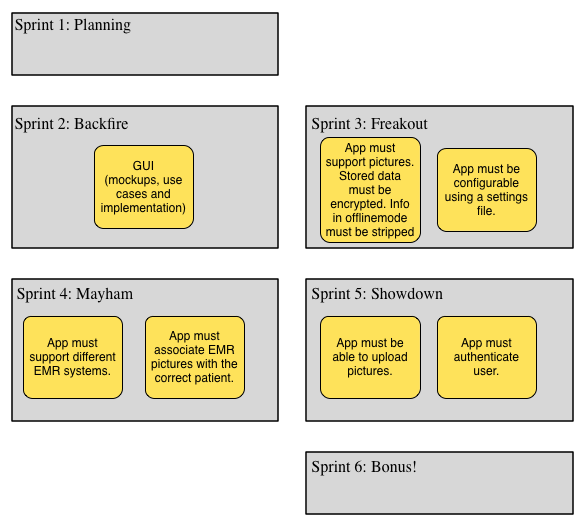
\includegraphics[scale=0.7]{img/sprint_overview.png}
\caption{Overview of the sprints and their goals}
\label{fig:sprinter_oversikt}
\end{figure}


\subsection{Work methodology}
Having some experience with Scrum, the group decided to go for an agile Scrum methodology. The focus was on frequent communication with the customer, use of agile collaboration software (see section \ref{project_management_tools}) and typical agile development practices like daily stand-ups. In this section, various agile concepts and how we used them in the project will be presented.


\subsubsection{Product backlog}
At the highest level, this is a set of stories describing the different functions of the system. These stories were broken up to a list of smaller, concrete issues. The customer had access to this list, and was able to add and subtract functionality as the product evolves.


\subsubsection{Planning and effort estimation}
With the product backlog as the basis, each task was estimated. The estimate represented how many hours we though were needed to complete a given task. This was initially meant to be re-done at the start of every sprint. However, due to the amount of research needed to be done throughout the project and the uncertainty about the extent of each task before we got in touch with the right experts, we abandoned this idea after the first sprint. The estimates were so far off they served no purpose.


\subsubsection{Sprint backlog}
Tasks were be estimated, prioritized and put into a \emph{backlog} containing all available tasks for the given sprint. Because the group was not given a requirements document in the beginning of the project, additional tasks were often added continuously in the sprint backlog when research revealed new requirements.


\subsubsection{Daily stand-up and work sessions}
Daily \emph{stand-ups} were arranged Monday through Friday. A stand-up meeting is a short meeting with all the team members where the purpose is to update each other on the project status and individual progress. Lasting no more than a total of 5-15 minutes, each team member should answer the following questions:
\begin{itemize}
     \item \emph{What have I done since the last meeting?}
     \item \emph{What will I do today?}
     \item \emph{Did I encounter any problems hindering my progress?}
\end{itemize}
\noindent
The group had mandatory work sessions at campus three times a week.


\subsubsection{Sprint end and demo}
At the end of each sprint, a few of the group members met with the customer and demonstrated a working version of the product. This opportunity was also used to discuss the backlog. Getting direct feedback from the customer could help point us in the right direction.
%It was also very helpful for us to get direct feedback while demonstrating the application at its current state.


\subsubsection{Sprint retrospective}
After each sprint, the team got together and looked at the past two weeks. Two key points were discussed in these meetings:

\begin{itemize}
     \item What went good?
     \item What went bad and/or should have been done different?
\end{itemize}
\noindent
It is important to identify both positive and negative parts about the sprints while they are still fresh in memory. That way the group knew what to focus on improving in the next sprint, and what to continue doing.

Based on experiences from the sprint retrospective meeting and feedback from the sprint end demo, the product backlog was re-evaluated.


\subsection{Milestones}
At the beginning of the project the group created milestones based on the limited information available. How these milestones were planned according to the sprints can be seen on the next page.

\begin{table}[H]
\begin{tabular}{p{2cm}p{11cm}}
%09.02.2014 & \emph{Preliminary version of the report:} A brief overview of work done up to this point, focusing on planning and organization. \\
14.02.2014 & \emph{Sprint 1 end:} Sprint end. \textbf{Milestone:} Ready to code. At this point the implementation can start. \\
28.02.2014 & \emph{Sprint 2 end:} Sprint end and product demonstration for the customer. \textbf{Milestone:} GUI ready for implementation. The plan for the GUI is ready and the usability test is done. \\
14.03.2014 & \emph{Sprint 3 end:} Sprint end and product demonstration for the customer. \\
%16.03.2014 & \emph{Mid-semester version of the report:} A more detailed overview of work done up to this point. Should contain an architecture and a plan for how to meet the requirements set. \\
28.03.2014 & \emph{Sprint 4 end:} Sprint end and product demonstration for the customer. \\
11.04.2014 & \emph{Sprint 5 end:} Sprint end and product demonstration for the customer. \textbf{Milestone:} Potentially shippable product \\
02.05.2014 & \emph{Sprint 6 end:} Sprint end and product demonstration for the customer. \textbf{Milestone:} Code freeze \\
%30.05.2014 & \emph{Final version of the report:} Deliver the complete report. \\
02.06.2014 & \emph{Product demo for the customer:} Demonstration of the final application for the customer. \\
\end{tabular}
\end{table}



\subsection{Risk management}
As suggested early on by the group's supervisor, getting a risk management plan ready was prioritized. A list of risks that could possibly threaten the project were set up. Having a plan is important to better tackle any problems should they arise. It is also a preventive measure, because it spreads awareness of potential problems to look out for. Risks have various consequences and potential impact on progress. Some are unavoidable and out of our hands, while others should be avoided at all cost. An example of the former is illness within the group. Risks are a product of two parameters: the probability of the loss happening and the consequence should the loss occur. A detailed description of identified risks can be found in Appendix \ref{risk}.

\section{Prestudy and research}
As mentioned in the project introduction, the quality of the final solution would rely on our ability to research and understand the medical industry. While both of the customers had experience with software development in this industry, their field of knowledge were mainly limited to the area of professional medical imaging. Based on this, the customer requested information about how other parts of the IT infrastructure worked, with a special focus on how to get patient data in and out of an electronic medical record. 

\subsection{Method}
Because of the need for extensive research, this chapter is not limited to "prestudies". Research spanned the whole project and had to be done in parallel with the development. The research method have revolved around getting a hold of and communicating with different key persons in the Norwegian industry, listed in Appendix \ref{contacts}. At the beginning of the project, the two biggest questions we set out to answer were: 

\begin{itemize}
\item How are the existing systems compiled?
\item What kind of systems will the application be dependent on?
\end{itemize}

As discovered, uploading directly to an "EMR" was not necessary the solution. In this chapter, we will present the findings of how the Norwegian industry and environment work. This implies that some details about systems will differ from hospital to hospital. In order to avoid confusion we will start by presenting terminology and technology in a historical context, commenting the extent of our research along the way.

\subsection{The history of EMRs}
\label{sec:history}
In the 1960s and '70s, early efforts were done to utilize computers in order to store and manage medical records overseas. Aerospace manufacturer Lockheed Martin developed one such system, a \emph{clinical information system} as they were called \cite{ehrDevelopment}. Already in the 1980s, one started to see the benefits of industry-wide standards. This led to the first initiative to standardize this information, and nonprofit standards developing organizations (SDOs) started to form. They would facilitate the widespread use and organization of electronic medical information.
\noindent
One of these initiative takers was Health Level 7 (HL7). Since 1987 they have became the most widely recognized SDO in the industry of medical information technology. They develop electronic standards to ensure that the different departmental systems can exchange clinical data in a meaningful way. This is essential because modern hospital information systems (HIS) are often composed of components made by many different vendors. Since the beginning, HL7 have released numerous messaging standards. With a coverage of 95\% in the US healthcare organizations, HL7v2 is by far the most used messaging protocol for clinical data today \cite{hl7numbers}. A discussion on HL7 and other standards follows later in this chapter.

\subsection{Medical imaging}
The installation of a platform to organize medical images, like the one Lockheed Martin developed for the EMRs in the mid 60s, saw the light of day in 1982. This platform was called a Picture Archiving and Communication System (PACS). With new image management systems emerging, the radiographic community saw the need for a standardized format these systems could utilize. In 1985 The American College of Radiology (ACR) and National Electrical Manufacturers Association (NEMA) released their first standard. It was called ACR/NEMA 300, but would later be recognized as the Digital Imaging and Communications standard (DICOM). 
Like HL7 is the industry standard for text based clinical information, DICOM is the industry standard for handling, storing and transmitting data in medical imaging today \cite{dicom_standard}. As the name suggest this standard include both a file format e.g. a way of structuring the data, as well as a protocol to transport it over. 

This was the first format we set out to explore. As this is the most used format and protocol for medical imaging, we thought a PACS would be the place to upload images to. Based on that information, we spent a good amount of time learning the details in this standard in order to upload images.

%%%%%%%%%%%%%%%%%%%% NY SUBSECTION %%%%%%%%%%%%%%%%%%%%


\subsection{Understanding the environment}
\label{sec:understandingEnvironment}
In this section we will first give an explanation of the central interoperability issues existing in today's systems, before we explain how a typical hospital IT environment is structured.

As mentioned, a modern hospital information system (HIS) can be compiled of multiple, both dependent and independent software solutions from different vendors. Below we will discuss the connection between selected solutions.
\noindent
The common denominator between the components that constitute the HIS, is the messaging protocols standardized by the SDOs. As mentioned earlier, this is the gap HL7 set out to fill. Already in 1989 HL7 introduced their HL7v2 standard. An example of a HL7v2 message can be seen in Figure \ref{fig:hl7sample}. Here, fields are separated by pipes, hence the nickname \emph{Pipehat}:

\begin{figure}[H]
\centering
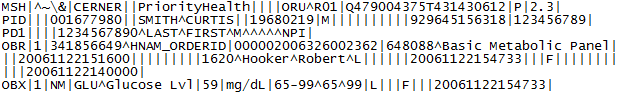
\includegraphics[scale=0.8]{img/hl7sample.png}
\caption{HL7v2 sample message}
\label{fig:hl7sample}
\end{figure}

\noindent
As HL7v2.x was the most used messaging protocol by far, the group initially thought our solution depended on our understanding of this standard in order to get patient data from a hospital information system.

To date there has been released 9 versions of HL7v2, represented generically as HL7v2.x. Although the v2.x standards are backward compatible, it does not have the strongest foundation; it was built in a "bottom-up" approach that has addressed individual needs. There is no underlying reference model and the first version was released only two years after the HL7 organization was founded. With 25 years of infrequent additions to the standard it is loosely defined and suffers - as others have suggested \cite{evolution:hl7} and \cite{rel:openehr} - from too much optionality. Because of this, situations where two systems supporting HL7v2 don't necessarily interoperate occur, because they implement different parts of the standard. This again has led to additional initiatives like the Integrating Healthcare Enterprise (IHE) \cite{ihe} which is focusing its work into specifying integration \emph{profiles} based on clinical domains. In other words, they are trying to standardize different parts of an existing standard. This is also adversely, as hospitals end up using different profiles that don't work together.
Typically, a hospital IT infrastructure is built around a centralized patient administration system (PAS). Surrounding it is several departmental systems, such as those for laboratory, radiology etc. A system for managing medical records is usually closely associated with the PAS, hence the commonly used abbreviation PAS/EMR. These services are made accessible through terminals stationed at individual departments usually running the Windows operating system. As we've learned (Heidi Torstunsen, personal communication, February-April, 2014), the hospitals strive to keep the number of credentials associated to one person to a minimum, and they are often identical across different logins. Despite the central PAS/EMR, departmental systems may also have their own systems for managing information about patients treated there. As Roald Bergstrøm told us, this is the case in the radiology department: Here the PACS gets patient information from a radiology information system (RIS) (meeting, February 28, 2014). Overlapping systems like this is not uncommon in the hospital environment; it has do with the concurrent development of the individual systems. The PACS exchanges textual metadata directly to the EMR in form of a \emph{report}. This happens via HL7 messages, as seen in Figure \ref{fig:theEnvironment} on the next page. This means that some information about a patient's radiology examination can be found in the PAS/EMR. The whole examination with images can be viewed through a web view connecting to the PACS where the images are stored.

\begin{figure}[H]
\centering
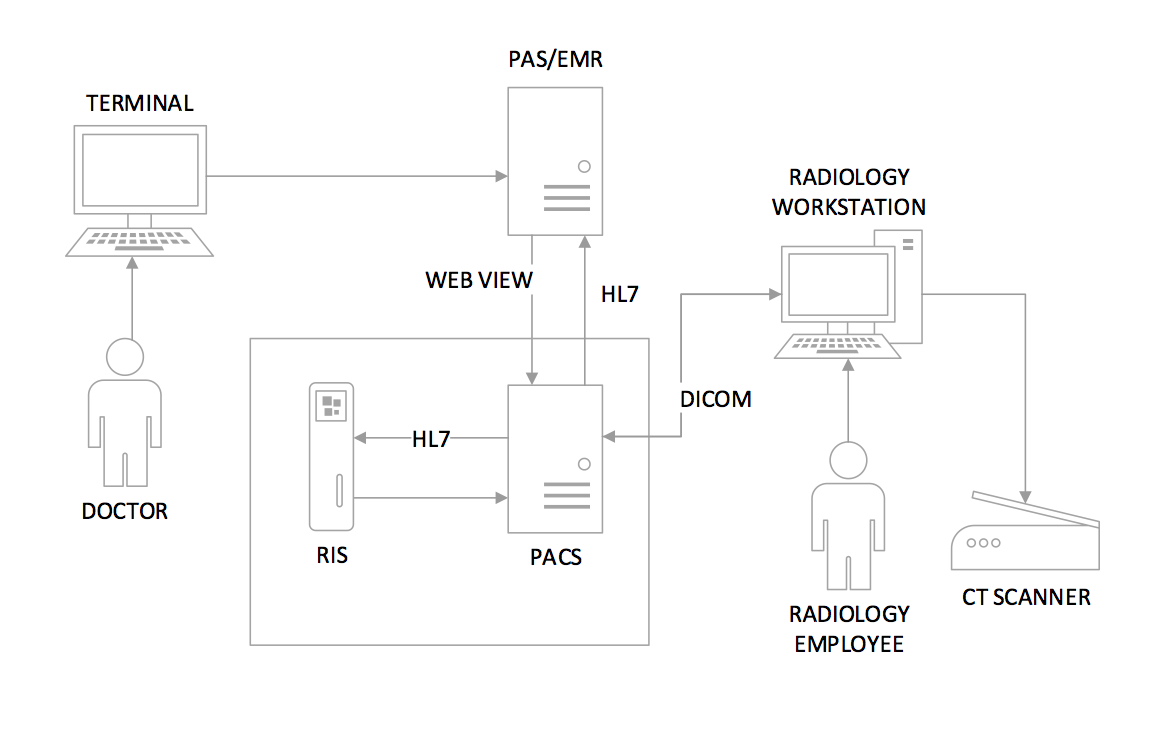
\includegraphics[scale=0.6]{img/env_chart.png}
\caption{A selected portion of the environment}
\label{fig:theEnvironment}
\end{figure}


%%%%%%%%%%%%%%%%%%%% NY SUBSECTION %%%%%%%%%%%%%%%%%%%%

\subsection{Today and the future}
After sprint 4, described in section \ref{sprint4}, it was decided to put some additional effort into researching future solutions and standards. This section will cover the work that is currently being done in the industry in order to solve interoperability issues in today's systems.

\subsubsection{HL7v3 and openEHR}
Despite it's popularity, even HL7 acknowledged that v2.x had some legacy issues. To avoid the burden of the these issues, they decided it would not be backward compatible. Starting from scratch they first defined a reference information model (RIM) \cite{hl7RIM}, which they based the third messaging standard, HL7v3 on. These messages have a more familiar XML syntax.

Through conversations with Roald Bergstrøm from KITH \cite{KITH}, we were introduced to what the future holds for hospital IT infrastructure and electronic medical records. He told us that in Australia, a group of researches spent more than 15 years of research to develop and test an open, detailed and comprehensive interoperable health information computing platform. Its called openEHR \cite{openEHR}, and is based on a two-level modeling approach, known as the ‘archetype methodology’. Archetypes is a way of structuring data, where you clearly define clinical information models. This makes it possible to separate a information system's data model from the clinical one. Several SDOs believe this is the future for interoperable data between clinical systems and shared EMRs. Over the last couple of years, the architecture have influenced the development of EHR standards by both CEN (European Committee for Standardization), HL7 and ISO (International Organization for Standardization) \cite{rel:openehr}. In Norway the process of defining, quality assure, approve and share archetypes on a national scale was initiated by the The Western Norway Regional Health Authority \cite{helseVest}, and is currently in progress.

Based on this methodology, HL7 released a standard document structure specifying the structure and semantics of clinical documents. It is called Clinical Document Architecture (CDA) and is based on XML Schemas \cite{hl7CDAR2}. These documents are still thought to be exchanged by the HL7v3 messaging standard. The standard is currently in its second release (CDA R2), and have already been adopted by DIPS (see section \ref{exsol}). Figure \ref{fig:HL7relationship} illustrates the relationship between openEHR, CEN13606 and HL7. For more information, see Ocean Informatics article on the relationship between CEN 13606, HL7, and openEHR\cite{rel_openehr1}.

\begin{figure}[H]
\centering
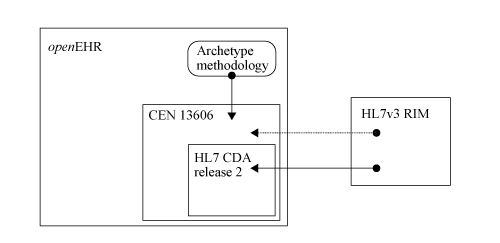
\includegraphics[scale=0.8]{img/relationship.png}
\caption{The relationship between openEHR and HL7\cite{rel_openehr1}}
\label{fig:HL7relationship}
\end{figure}



%%%%%%%%%%%%%%%%%%%% NY SUBSECTION %%%%%%%%%%%%%%%%%%%%


%%THE VSCAN DEVICE
\subsection{The Vscan device and ultrasound}
\label{vscan}
The existing Vscan device is a handheld, pocket-sized visualization tool powered by ultrasound technology. The device was first introduced in 2010, after being developed by GEs Norwegian department GE Vingmed, based in Horten. The device is bundled with a desktop application called Gateway, which allows for importing and organizing images and video. This is done through a docking station that is connected to the computer via an USB cable. The latest version of this software support reporting capabilities by generating PDF (Portable Document Format) reports from an examination. An example report can be found in Appendix \ref{existingGatewayReport}.

The customers intend to improve the original Vscan product. At the first meeting the group were told that GE had reason to believe that all ultrasound specific technology some time in the future would be able to fit inside the probe (Figure \ref{fig:ultraprobe}.b) of the existing product. With these ultrasound probes in mind, the customer envisioned the ability to connect it to a modern smart device (like a smart phone Figure \ref{fig:ultraprobe}.a) over a standard interface like the Universal Serial Bus (USB). These smart devices would then run software applications with a user interface for the scanner.

\begin{figure}[H]
\centering
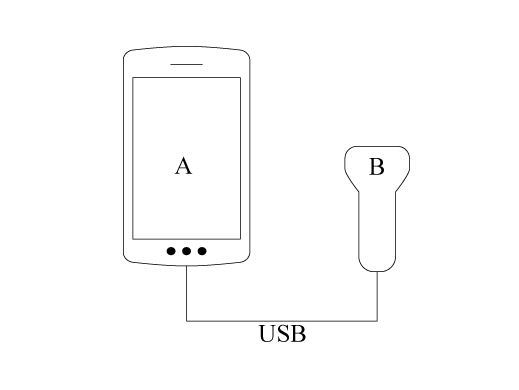
\includegraphics[scale=0.4]{img/ultraprobe.png}
\caption{Smart device (a) with attached ultrasound probe (b)}
\label{fig:ultraprobe}
\end{figure}

\noindent
Although GE developed the first device of this kind, they are not alone on the market: The customer told us that they considered Siemens hand held ultrasound system \cite{ACUSONP10} to be their main competitor. We have found other devices with even greater similarities to the  smart device (with interchangeable probes) solution they now envision \cite{MobiUSSP1}.

The original device and its competitors have introduced the term \textit{pocket ultrasound}. Traditionally ultrasound examinations are performed by professional radiologists or technicians at a radiology department. With pocket ultrasound this workflow changes, and examinations can be conducted in the patient rooms. This improvement in technology opens for more frequent use of ultrasound, and the user group will no longer be restricted to those working in the radiology department. 

The implications of this was \emph{not} obvious to the group at first, as we initially thought the application could rely on PACS for storing ultrasound images. After a detour exploring PACS and DICOM, we realized that uploading data to PACS was impossible, as this was a system exclusively for the radiology department, and unavailable for other medical personnel. Another solution had to be found.


%%%%%%%%%%%%%%%%%%%% NY SUBSECTION %%%%%%%%%%%%%%%%%%%%


\subsection{DIPS}
\label{exsol}
From October this fall, DIPS will be installed at OUS. This combined with their marked share, is the reason we invested time in researching their solutions. 

The same year HL7 started its work, the Norwegian company DIPS (Distribuert Informasjons og Pasiendatasystem i Sykehus) was founded at Nordland Sentralsykehus. They set out to develop \emph{''user friendly software that run on standard hardware in a network''}. Today, they have extended their product line and offer modules for EMR, PAS, Multimedia and Economy to name a few. With more than 70\% coverage of Norwegian hospitals, they are currently Norway's largest vendor of EMR software \cite{DIPS}, with customers in three of the four Regional Health Authorities in Norway \cite{RHF}. They were also the first EMR company in Norway to implement support for many standardized system-to-system protocols, utilizing XML (Extensible Markup Language) and HL7 standards \cite{dips_pioneer}.

Initially, OUS  will get the solution DIPS Classic, which is their old PAS/EMR solution. Through communicating with Konik developers working on integrating this solution in Oslo, the group was given access to an empty DIPS server as described in section \ref{serviceDescription}. 

After communication with Alexander Theodorsen, working at DIPS in Bodø, we got some insight on how their solutions worked, and how it would affect our application. Among other things, he informed us that \emph{Active Directory} was the main user management system used by hospitals in Norway. Based on this, LDAP was chosen as the applications authentication mechanism.


%%%%%%%%%%%%%%%%%%%%%%%%%%%%%%%%%%%%%%%%%%%%%%%%%%%%%%%%%%%

\subsection{Multimedia in hospitals}
\label{multimediaInHospitals}
The storing of images and video on hospital servers are today almost exclusively used by radiologists, but there is a demand for multimedia and smart mobile devices. Researchers think this will become a more central aspect of the daily patient care in the future \cite{indremedisineren}. As mentioned in the introduction of this chapter, a big question for this project resided in where the results of an examination should be stored. As we've covered in the previous sections, we put a good amount of effort into researching systems like PACS and the core EMR in order to store information from our application. Because of the clinical value radiologists add in the PACS, ultrasound images from hand held devices did not belong here. Although DIPS (as an example) support PDF attachments to be uploaded in the actual EMR, these systems are specialized around text-based documents, and do not meet the needs for searching and indexing multimedia. Another issue was pointed out by Heidi Torstunsen (communication, 2014), who told us that current laws and regulations put restrictions on what data that can be stored; only data of a certain clinical value should be stored. Roald Bergstrøm at KITH could confirm this, and said the following:
\newpage
\begin{quote} 
\textit{A national selection has evaluated whether images should be stored in the EMR, and has concluded that the findings of the doctors is the artifact to be considered legally binding. This entails that when ultrasound images are examined and described, this description is applicable and should be saved while the image can be deleted. \\(Translated from Norwegian)}
\end{quote}
\noindent
However, Roald himself consider this to be bad practice and pointed out that X-ray images are saved up to 10 year for further reference. Taking the needs of the customer, as well as feedback we got from stakeholders in the industry into consideration, we decided to not take this into account, as it would end our project. After consulting with the customer we decided to continue researching other possible, future solutions. 

To this date there is no widely recognized system for storing multimedia. The only solutions we could find was \emph{DIPS Multimedia} \cite{dipsmultimedia} and \emph{Seekuence} from Posicom \cite{posicom} which are currently being tested and deployed. These are both pioneers in this market. Both systems takes the form of independent modules ready to be integrated with existing hospital systems like PAS/EMR, and they are built on modern technology supporting a wide array of multimedia formats and protocols. We have yet to figure out how they cope with the issues regarding national rules and regulations in their solutions.

We worked with Bjørn Næss (personal communication, March - May, 2014) to get help implementing a service communicating with DIPS Multimedia. As this solution is still being tested, DIPS did not have any development documentation for us. Bjørn tried to arrange for us to get help from one of their developers, but due to time constraints it did not work out.

%%%%%%%%%%%%%%%%%%%% NY SUBSECTION %%%%%%%%%%%%%%%%%%%%


\subsection{Security}
Security is a topic that can not be avoided when developing software for this industry. In the following section we will give an overview of the most important issues we encountered. After a section on mobile smart devices and memory, we conclude with a simple risk assessment.

\subsubsection{Smart devices}
We believe some consideration regarding possible hardware threats is of interest to the customer. Both Heidi Torstunsen could tell us that devices like this are bought in, and managed at a department level. This means that the department share one or more hand held devices. Due to security reasons, this is likely to stay the same even with the introduction of smart devices. A Bring Your Own Device (BYOD) policy is currently not applicable for clinical devices. From a security point of view, there are a lot of challenges with having a single device shared between multiple unique users. This is outside the scope of this project, but we believe it is important to point out.

To illustrate some of the security concerns regarding mobile smart devices, we have written a short article on possible threats, if the customer should be interested. Based on this research, we concluded to not consider in app memory when assessing the security aspects of our application. Because of this we decided not to include it in the final report. It can be found in Appendix \ref{smartSecurity}.


\subsubsection{Risk assessment}
Through communication with Heidi Torstunsen, responsible for privacy and information security at OUS. Many of the design decisions are a direct result of what she told us and the documents she made accessible. We have designed our application with the concerns from OUS's guidelines in mind \cite{ousDocuments_riskAssesment}. As Heidi stated, the Norwegian rules and regulations on privacy and security are considered strict compared to other Europeean countries. We believe this was a healthy base for our design.

Considering the amount of data stored in the application i.e. the number of patients whose sensitive data is in memory at a given time, the individual customers could do a risk assessment and either acknowledge or reject the risk. The way we see it, this number would typically be low, because only examinations intended to be uploaded (at some point) should enter the application. When uploaded, the examination is deleted. 

The real risk as we see it, is the potential loss of user credentials. Concrete examples on how this could be done is found in Appendix\ref{smartSecurity}. Depending on the national and local policy for access control, this could give the attacker access to information about patients on a department, hospital, regional or national level. 


%%%%%%%%%%%%%%%%%%%% NY SUBSECTION %%%%%%%%%%%%%%%%%%%%

%%STAKEHOLDERS
\subsection{Stakeholders}
When making products for the medical industry, there are a lot of people involved with different interests. In this section, the different stakeholders will be presented.

\subsubsection{Product owner}
The group's contact at Capgemini is Jens Lien. Because he is hired by GE, he is acting on their behalf and therefore considered to be the product owner. He has previous experience with developing software for the medical business, and has a vision for what is to be built. His concerns are: 

\begin{itemize}
\item The application works as intended.
\item The application is finished in the given time period.
\end{itemize}

\subsubsection{Application vendor}
Sigmund Frigstad is a project leader at GE Vingmed, and was in charge of developing the original Vscan device. He is responsible for the Vscan device that the application will be shipped with. His concerns are: 

\begin{itemize}
\item The application runs on the specified platform/hardware.
\item The application communicates with the Vscan application.
\item The application is able to communicate with hospital servers.
\end{itemize}

\subsubsection{End user}
This is the group of users that will use the Vscan device and the application in the hospitals. This group is divided in two; technical users and non-technical users. Non-technical users users are considered to be doctors and other medical personnel certified to perform examinations with a pocket ultrasound device \cite{EFSUMB}. The technical users are considered to be technical staff working at the hospitals. Their concerns are respectively:\\

\textbf{Non-technical user}
\begin{itemize}
\item The application is intuitive to use and eases the work flow of storing ultrasound images.
\item The application is able to save changes before uploading data.
\end{itemize}

\textbf{Technical user}
\begin{itemize}
\item The application can be set up to work with the hospital servers.
\item The need for manual inputting data is minimal when setting up device.
\end{itemize}
\noindent Non-technical users will be referred to as users in the remainder of the report.


\subsubsection{System owner}
This stakeholder can either be the hospital administration itself or an external company delivering systems or services to the hospital. An example of a relationship like this is the Norwegian institution Sykehuspartner \cite{sykehuspartner}. The system owner is responsible for setting requirements for availability, confidentiality, integrity and quality of the systems delivered to, or used on the respective hospital institutions. Their concerns are:

\begin{itemize}
\item That the application meets legal requirements when handling personal information in an hospital environment.
\item That the application meets security requirements set by the specific hospital, district, region or country.
\end{itemize}

\subsubsection{Third-party Developer}
A developer will be needed to customize certain parts of the solution at the individual hospitals. Their concerns are:

\begin{itemize}
\item Good API documentation.
\item All data necessary to upload examination is available.
\end{itemize}


%%%%%%%%%%%%%%%%%%%% NY SUBSECTION %%%%%%%%%%%%%%%%%%%%


%DEV TOOLS AND LIBS
\subsection{Libraries and development tools}

A number of tools and libraries have been used during development of the application. Some of them were required by the customer, but most have been chosen based on the groups preference and experience, and most importantly, because they fit the project needs. A requirement for all the applications used, is that they are free to use and multi platform, as the group got members using both Windows and Mac OSX. It was determined that tools for the following purposes were needed:

\begin{itemize}
\item Development
\item File storing and version control
\item Documentation
\item Communication
\end{itemize}

%DEV TOOLS
\subsubsection{Development tools}
This section contains an overview of the development tools and libraries used in the project.
\paragraph*{Android and Java}
Android is an operating system developed and maintained by Google aimed at smartphones and tablets. The Android platform is released under an open source license and has a large community of developers developing third party libraries and tools. Android is currently the most used mobile operating system in the world \cite{android_pop}. Applications developed for Android are written mainly in Java by using the Android software development kit (SDK), which are highly maintained and very well documented.

The application developed during this project was made for the Android platform. This was a requirement set by the customer and the basis for the project.

\paragraph*{IntelliJ IDEA}
IntelliJ IDEA \cite{intellij} is an IDE (Integrated Development Environment) which supports Android and has integrated support for all major build tools. The build tool support was an important consideration when choosing an IDE, as it may be both hard and time consuming to maintain a large project with many dependencies. The group were recommended to use IntelliJ by the customer representative at Capgemini.

\paragraph*{Genymotion}
When developing for Android, either an emulator or a physical device is needed to simulate the runtime environment for an application. The Android SDK comes bundled with a standard emulator, but it is extremely slow and a hassle to work with. Therefore, the group have been using the Genymotion \cite{genymotion} emulator which is based on Oracle VirtualBox \cite{virtualBox}. Genymotion has increased performance compared to the standard emulator.

\paragraph*{Gradle}
When maintaining a large project, a build tool is very helpful. Gradle \cite{gradle} is a build tool made specifically for Android development. It helps with everything from managing third party libraries and other dependencies, to compiling the project.

%%LIBS
\subsubsection{Libraries}
This section contains an overview of the libraries used in the project. All libraries are free to use, and most are open source.

\paragraph*{SQLite and SQLCipher}
SQLite is an open source, lightweight database management system (DBMS) which is included as a standard in all Android based devices. It is simple to use, universal and got all the functionality needed. Because of its popularity, there are several libraries offering encryption of databases on Android devices running on top of SQLite. The open source project SQLCipher \cite{sqlcipher} was chosen as it offered easy integration with our existing database. SQLCipher offers AES 256 bit encryption.

\paragraph*{Crouton}
Crouton \cite{crouton} is a library which serves as an alternative to the traditional Android \textit{Toast} \cite{toast}. A Toast is a small popup notification that floats on the screen for a given time. The problem with Toast for our use, is that Toasts are context in-sensitive, meaning they do not "belong" to their parent view and will not disappear before they have run their full duration. This could possibly make for some confusing situations for the user, with multiple Toasts floating on the screen. This is where Croutons come in. A Crouton is context sensitive, meaning it will dissapear once its parent view is hidden or removed.

\paragraph*{FlatUI kit and PhotoView}
FlatUI kit \cite{flatui} and PhotoView \cite{photoview} are both libraries used to enhance the UI of the application. The FlatUI kit offers easy integration of attractive UI elements as an alternative to the standard Android look and feel. PhotoView is used to ease the implementation of functionality like zooming and multi-touch gestures in ImageViews.

\paragraph*{UnboundID LDAP}
UnboundID \cite{unboundid} is a SDK for Java, used to provide Lightweight Directory Access Protocol (LDAP) functionality in the application. 

\paragraph*{JCraft JSch}
JSch \cite{jsch} is used in the Android service, and is a library that allows connection to a server through the SSH protocol. 

\paragraph*{iText}
\label{itextlib}
iText \cite{itext} is a library that allows users to both generate and manipulate PDFs. 

\paragraph*{JDBC}
JDBC is used in the Android service, and is a library that allows for communication with a SQL database in Java \cite{JDBC}.
% OBS OBS! Bør skrive om JDBC (brukt i service)

%DOCUMENTATION TOOLS
\subsubsection{Documentation tools}
This section contains an overview of the tools and services used to document code, project process and report writing. See section \ref{project_management_tools} for additional tools used for project management. 

\paragraph*{Git and GitHub}
Git \cite{git} is an open source distributed version control system. Using a version control system allows multiple developers to work on the same code and commit their work to a common repository. Other participants then fetch these changes to their local copy of the repository. Git offers many advanced features. Most importantly, the group has been actively using the branching feature, which allows for different "copies" of the project to be worked on simultaneously. This is useful when implementing features that shouldn't be merged into the main project before they are fully implemented and working as intended. The group were assigned a private repository hosted at GitHub \cite{github} owned by the customer. This way the customer was able to follow the project progress closely.

\paragraph*{Javadoc}
Javadoc \cite{javadoc} is a widely used API documentation generator for Java. Javadoc generates documentation to HTML-format based on the contents of predefined tags inside the Java project source code. The group prioritized documenting the most important classes and interfaces of the solution.

\paragraph*{\LaTeX}
\LaTeX\ \cite{latex} is a document preparation system. It is widely used by academic institutions and has several advantages over word processors like Microsoft Word. Supporting large documents with a strict layout is easy with \LaTeX\ . The source can be written in separate text files and merged together when building. This allows for multiple users to work on the same document without conflicts.

\paragraph*{Google Drive}
For storing and working with documents related to the project, the group has used Google Drive \cite{googledrive}. This platform allows all members of the group easy access to documents, and also offers the opportunity for multiple users to work on the same documents at the same time.
\include{libraries_and_devtools}
\section{Requirements}
\label{requirements}
In this chapter, the requirements for the system will be described. Project requirements is a list of the functionality an application must both uphold and support; the criteria on which to judge the application on. As stated earlier, the customer wanted us to explore what possibilities existed for a future Vscan smart device. To not restrict our imagination, the group did not receive a requirements specification from the customer. With the little knowledge we had about the industry at the time, we had to come up with a strategy for how to define these requirements. Exactly how this was done, can be read about in section \ref{workbreakdown}.

\subsection{Business goals}
The main business goal was to improve the usability and effectiveness of the Vscan device. Other goals were to reach out to as large part of the target marked as possible. To realize this, the application had to be easy and fast to use and needed to support integration with legacy systems. This involved being scalable to the extent where the cost of implementing support for a new system was minimal.

\newpage

\subsection{Functional requirements}
The functional requirements describes the concrete functionality the system is required to uphold. Table \ref{funcreqtable} is the full list of functional requirements for the application.


%Tabell for functional requirements
\begin{center}
\tablefirsthead{\hline  \multicolumn{1}{|c}{\tbsp \textbf{FR\#}}
                       & \multicolumn{1}{c}{\textbf{Description}}
                       & \multicolumn{1}{c|}{\textbf{Priority}} \\ \hline\tbsp  }
\tablehead{\hline \multicolumn{3}{|l|}{\small\sl continued from previous page}\\
           \hline \multicolumn{1}{|c}{\tbsp \textbf{FR\#}}
                       & \multicolumn{1}{c}{\textbf{Description}}
                       & \multicolumn{1}{c|}{\textbf{Priority}} \\ \hline\tbsp  }
\tabletail{\hline\multicolumn{3}{|r|}{\small\sl continued on next page}\\\hline}
\tablelasttail{\hline}
\par
\captionof{table}{Functional requirements}

\begin{supertabular}{|p{1cm}|p{9cm}|p{2cm}|}
\label{funcreqtable}

1 & \begin{tabular}[c]{@{}l@{}}
At first startup the application must allow tech-\\
nical personnel to correctly set up the EMR\\
system in use at the current hospital
\end{tabular}  & High \\ \hline

2 & \begin{tabular}[c]{@{}l@{}}
The application must be able to receive images\\
from the Vscan-application
\end{tabular} & High \\ \hline

3 & \begin{tabular}[c]{@{}l@{}}
The application need to allow doctors to authen-\\
ticate with the EMR-system
\end{tabular} & High \\ \hline

4 & \begin{tabular}[c]{@{}l@{}}
The application must be able to identify patients \\
based on SSN
\end{tabular} & High \\ \hline

5 & \begin{tabular}[c]{@{}l@{}}
The application need to be able to upload images \\
to the hospital servers
\end{tabular} & High \\ \hline

\iffalse
2 & \begin{tabular}[c]{@{}l@{}}
The application need to be able to communicate with a interchangeable service over a common interface that\\
is responsible for communication with the EMR itself
\end{tabular} & High \\ \hline
\fi

6 & \begin{tabular}[c]{@{}l@{}}
The application must be able to identify patients \\
based on barcode/QR-code
\end{tabular} & Medium \\ \hline

7 & \begin{tabular}[c]{@{}l@{}}
The application must give feedback to the user\\
on what patient have been identified
\end{tabular} & Medium \\ \hline

8 & \begin{tabular}[c]{@{}l@{}}
The application need to be able to associate ima-\\
ges with the correct patient
\end{tabular} & Medium \\ \hline

9 & \begin{tabular}[c]{@{}l@{}}
The application should let the user view images\\
contained in an examination
\end{tabular} & Medium\\ \hline

10 & \begin{tabular}[c]{@{}l@{}}
The application must not display sensitive infor-\\
mation if the application is in offline mode
\end{tabular} & Medium \\ \hline

11 & \begin{tabular}[c]{@{}l@{}}
An examination must be deleted from the device \\
after being successfully uploaded to the EMR
\end{tabular} & Medium \\ \hline

12 & \begin{tabular}[c]{@{}l@{}}
The application must auto-close and/or auto-log \\
out after a given time of inactivity
\end{tabular} & Medium \\ \hline

13 & \begin{tabular}[c]{@{}l@{}}
The application must be able to be used by more \\
than one user
\end{tabular} & Medium \\ \hline

14 & \begin{tabular}[c]{@{}l@{}}
The application must be able to save the current \\
examination to the database if interrupted before \\
finishing the examination procedure.
\end{tabular} & Medium \\ \hline

15 & \begin{tabular}[c]{@{}l@{}}
The application must be configurable through a \\
settings menu.
\end{tabular} & Medium \\ \hline

16 & \begin{tabular}[c]{@{}l@{}}
The doctor must be able to add comments on \\
associated pictures
\end{tabular} & Low \\ \hline

17 & \begin{tabular}[c]{@{}l@{}}
The doctor must be able to add comments on the \\
examination as a whole
\end{tabular} & Low \\ \hline

18 & \begin{tabular}[c]{@{}l@{}}
The settings view of the application must be pass-\\
word protected
\end{tabular} & Low \\ \hline

19 & \begin{tabular}[c]{@{}l@{}}
The application must support Android version 4 \\
and up
\end{tabular} & Low \\ \hline

\end{supertabular}
\end{center}


\newpage

\subsubsection{Use cases}
This section contains use cases for the high level functional requirements. They are listed both textual and as images to help understand their meaning.

\begin{table}[H]
\renewcommand{\arraystretch}{1.2}
\captionof{table}{Use case: Configuration}
\begin{tabular}{|p{4cm}|p{9cm}|}
\hline
Functional req. ID & 1 \\ \hline
Name & Configuration \\ \hline
Goal & \begin{tabular}[c]{@{}l@{}}
At first startup, the application must allow technical\\
personnel to set up the application to work with the \\
EMR system in use at the current hospital
\end{tabular} \\ \hline
Actors &  Technical user\\ \hline
Start requirements & \begin{tabular}[c]{@{}l@{}}
1.  A preconfigured settings file (XML) must be\\hosted on an available HTTP-server\\
2. The application is deployed to the device
\end{tabular} \\ \hline
End requirements & \begin{tabular}[c]{@{}l@{}}
The application is correctly configured, and is ready\\ for use
\end{tabular} \\ \hline
Main flow & \begin{tabular}[c]{@{}l@{}}
1. User gets prompted to set a technical password\\
2. Writes and repeats password and clicks “OK”\\
3. User gets prompted to input URL to settings file\\
4. Inputs URL to settings file and clicks “Get config”\\
5. Clicks “Confirm”\\
6. User gets prompted to input department username\\/password\\
7. Inputs department username/password and clicks\\ “Confirm”
\end{tabular} \\ \hline
Alternative flow & \begin{tabular}[c]{@{}l@{}}
2a: The technical password (inputed twice) does not\\ match, and the user gets an error message\\
4a: The URL is invalid, and the user gets an error\\ message
\end{tabular} \\ \hline
Parent use case & None \\ \hline
Child use case & 3, 4, 5 \\ \hline
\end{tabular}
\end{table}


\newpage

\begin{figure}[H]
\centering
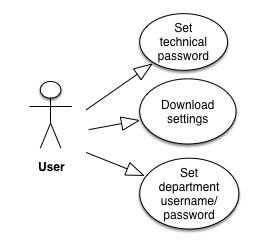
\includegraphics[scale=0.8]{img/usecase/usecase_config1.png}
\caption{Configuration}
\label{fig:config}
\end{figure}

\newpage

\begin{table}[H]
\renewcommand{\arraystretch}{1.2}
\captionof{table}{Use case: Receive images}
\begin{tabular}{|p{4cm}|p{9cm}|}
\hline
Functional req. ID & 2 \\ \hline
Name & Receive images from Vscan \\ \hline
Goal & \begin{tabular}[c]{@{}l@{}}
Receive images from Vscan
\end{tabular} \\ \hline
Actors &  User\\ \hline
Start requirements & \begin{tabular}[c]{@{}l@{}}
1. Vscan provides images ready to be uploaded
\end{tabular} \\ \hline
End requirements & \begin{tabular}[c]{@{}l@{}}
Images are received by the application
\end{tabular} \\ \hline
Main flow & \begin{tabular}[c]{@{}l@{}}
1. The Vscan application triggers the start of the\\ application.
\end{tabular} \\ \hline
Alternative flow & \begin{tabular}[c]{@{}l@{}}
None
\end{tabular} \\ \hline
Parent use case & None \\ \hline
Child use case & None \\ \hline
\end{tabular}
\end{table}



\begin{figure}[H]
\centering
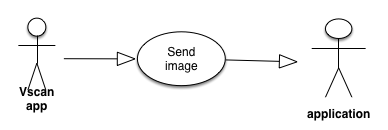
\includegraphics[scale=0.8]{img/usecase/receive.png}
\caption{Receive images from Vscan}
\label{fig:receive_image_uc}
\end{figure}

\newpage

\begin{table}[H]
\renewcommand{\arraystretch}{1.2}
\captionof{table}{Use case: Login}
\begin{tabular}{|p{4cm}|p{9cm}|}
\hline
Functional req. ID & 3 \\ \hline
Name & Login \\ \hline
Goal & \begin{tabular}[c]{@{}l@{}}
To login successfully
\end{tabular} \\ \hline
Actors &  User\\ \hline
Start requirements & \begin{tabular}[c]{@{}l@{}}
1. Login page is displayed\\
2. The user is registered in the system
\end{tabular} \\ \hline
End requirements & \begin{tabular}[c]{@{}l@{}}
The user is successfully logged in
\end{tabular} \\ \hline
Main flow & \begin{tabular}[c]{@{}l@{}}
1. The user gets prompted for username/password\\
2. Inputs username/password and clicks “Login”
\end{tabular} \\ \hline
Alternative flow & \begin{tabular}[c]{@{}l@{}}
2a: Username/password combination is wrong, and\\the
user gets an error message
\end{tabular} \\ \hline
Parent use case & 1 \\ \hline
Child use case & 4, 5 \\ \hline
\end{tabular}
\end{table}


\begin{figure}[H]
\centering
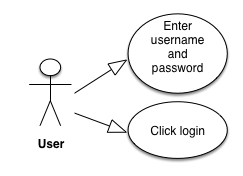
\includegraphics[scale=0.8]{img/usecase/login1.png}
\caption{Login successfully}
\label{fig:login_uc}
\end{figure}

\newpage

\begin{table}[H]
\renewcommand{\arraystretch}{1.2}
\captionof{table}{Use case: Identify}
\begin{tabular}{|p{4cm}|p{9cm}|}
\hline
Functional req. ID & 4 \\ \hline
Name & Identify patient \\ \hline
Goal & \begin{tabular}[c]{@{}l@{}}
Identify patient and retrieve patient data
\end{tabular} \\ \hline
Actors & User\\ \hline
Start requirements & \begin{tabular}[c]{@{}l@{}}
1. Identify patient view is displayed\\
2. User has patients SSN\\
3. Patient exists\\
4. The device has internet connection
\end{tabular} \\ \hline
End requirements & \begin{tabular}[c]{@{}l@{}}
The patient is identified, and patient data is retrieved
\end{tabular} \\ \hline
Main flow & \begin{tabular}[c]{@{}l@{}}
1. User gets prompted to input SSN\\
2. User inputs SSN and clicks “OK”
\end{tabular} \\ \hline
Alternative flow & \begin{tabular}[c]{@{}l@{}}
2a: SSN is invalid, and the user gets an error message\\
\end{tabular} \\ \hline
Parent use case & 1, 3 \\ \hline
Child use case & 4 \\ \hline
\end{tabular}
\end{table}

\begin{figure}[H]
\centering
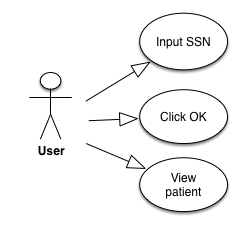
\includegraphics[scale=0.8]{img/usecase/identify1.png}
\caption{Identify patient}
\label{fig:identify_uc}
\end{figure}

\newpage



\begin{table}[H]
\renewcommand{\arraystretch}{1.2}
\captionof{table}{Use case: Upload images}
\begin{tabular}{|p{4cm}|p{9cm}|}
\hline
Functional req. ID & 5 \\ \hline
Name & Upload images to EMR \\ \hline
Goal & \begin{tabular}[c]{@{}l@{}}
Upload examination images to EMR
\end{tabular} \\ \hline
Actors &  User\\ \hline
Start requirements & \begin{tabular}[c]{@{}l@{}}
1. Application is correctly configured\\
2. User is logged in\\
3. Patient has been identified\\
4. Images has been received from Vscan\\
5. The device has internet connection
\end{tabular} \\ \hline
End requirements & \begin{tabular}[c]{@{}l@{}}
Images are uploaded to the EMR server
\end{tabular} \\ \hline
Main flow & \begin{tabular}[c]{@{}l@{}}
1. User is presented with “Review and Upload”-view\\
2. User scrolls down the page, reviewing the \\examination\\
3. User clicks ''Upload'' button\\
4. The application sends all necessary data to the \\service installed \\
5. The service acknowledges that the images were \\uploaded\\
6. The user is redirected to the “Home Screen”-view, \\
and is alerted that the examination was successfully \\uploaded
\end{tabular} \\ \hline
Alternative flow & \begin{tabular}[c]{@{}l@{}}
\textbf{2a)} User wishes to edit the notes before upload,
\\clicks the “Edit”-button, edits the notes and comes\\back to the “Review and Upload”-view \\
\textbf{3a)} User gets prompted with an alert dialog informing \\ that some of the images does not have notes attached\\
\textbf{5a)} Service was not able to upload examination, and \\
the user is returned to the “Home Screen”-view with\\ an alert dialog informing that the upload failed
\end{tabular} \\ \hline
Parent use case & 1, 2, 3, 4 \\ \hline
Child use case & None \\ \hline
\end{tabular}
\end{table}

\begin{figure}[H]
\centering
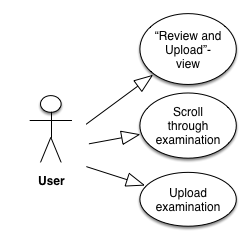
\includegraphics[scale=0.8]{img/usecase/upload1.png}
\caption{Upload images to EMR}
\label{fig:upload_uc}
\end{figure}

\newpage

\subsection{Quality attributes}
The non-functional requirements of a system describes the behavioral functionality required. This section includes a list of the non-functional requirements determined for the project.


\subsubsection{Mobility}
Mobility deals with the problems of movement and affordances of a platform. The scenarios focus on the availability and connectivity issues that might occur when using a mobile device.


\begin{table}[H]
\renewcommand{\arraystretch}{1.2}
\captionof{table}{Quality attributes: Mobility 1}
\begin{tabular}{|p{4cm}|p{9cm}|}
\hline

\textbf{MOB1} & \begin{tabular}[c]{@{}l@{}}
The user should be able to use the application when\\connected to the hospital intranet 
\end{tabular} \\ \hline 

\textbf{Portion of Scenario} & \textbf{Values} \\ \hline
Source of Stimulus & \begin{tabular}[c]{@{}l@{}}
User
\end{tabular} \\ \hline

Stimulus & \begin{tabular}[c]{@{}l@{}} 
Wishes to upload an examination with images and\\comments
\end{tabular} \\ \hline

Artifact & \begin{tabular}[c]{@{}l@{}} 
Smart device
\end{tabular} \\ \hline

Environment & \begin{tabular}[c]{@{}l@{}} 
Runtime with connectivity
\end{tabular} \\ \hline

Response & \begin{tabular}[c]{@{}l@{}} 
Examination successfully uploaded
\end{tabular} \\ \hline

Response Measure & \begin{tabular}[c]{@{}l@{}} 
Max 10 seconds
\end{tabular} \\ \hline

\end{tabular}
\end{table}


%%%%%%%%%%%%%%%	

\begin{table}[H]
\renewcommand{\arraystretch}{1.2}
\captionof{table}{Quality attributes: Mobility 2}
\begin{tabular}{|p{4cm}|p{9cm}|}
\hline

\textbf{MOB2} & \begin{tabular}[c]{@{}l@{}}
The application should manage network loss at any\\stage in its life cycle
\end{tabular} \\ \hline

\textbf{Portion of Scenario} & \textbf{Values} \\ \hline
Source of Stimulus & \begin{tabular}[c]{@{}l@{}}
User
\end{tabular} \\ \hline

Stimulus & \begin{tabular}[c]{@{}l@{}} 
Wishes to upload an examination with images and\\comments
\end{tabular} \\ \hline

Artifact & \begin{tabular}[c]{@{}l@{}} 
Smart device
\end{tabular} \\ \hline

Environment & \begin{tabular}[c]{@{}l@{}} 
Runtime without network connectivity
\end{tabular} \\ \hline

Response & \begin{tabular}[c]{@{}l@{}} 
Offline mode initiated
\end{tabular} \\ \hline

Response Measure & \begin{tabular}[c]{@{}l@{}} 
All examinations are saved locally
\end{tabular} \\ \hline

\end{tabular}
\end{table}


%%%%%%%%%%%%%%%


\subsubsection{Usability}
Usability is concerned with how easy it is for the user to accomplish a desired task. The scenarios focus on ease of use, learning, adaptation and configuration of the system.


\begin{table}[H]
\renewcommand{\arraystretch}{1.2}
\captionof{table}{Quality attributes: Usability 1}
\begin{tabular}{|p{4cm}|p{9cm}|}
\hline

\textbf{USA1} & \begin{tabular}[c]{@{}l@{}}
The application fits into the already existing workflow
\end{tabular} \\ \hline

\textbf{Portion of Scenario} & \textbf{Values} \\ \hline
Source of Stimulus & \begin{tabular}[c]{@{}l@{}}
User
\end{tabular} \\ \hline

Stimulus & \begin{tabular}[c]{@{}l@{}} 
Wishes to incorporate the application in an already\\existing everyday workflow.
\end{tabular} \\ \hline

Artifact & \begin{tabular}[c]{@{}l@{}} 
System
\end{tabular} \\ \hline

Environment & \begin{tabular}[c]{@{}l@{}} 
Normal operation
\end{tabular} \\ \hline

Response & \begin{tabular}[c]{@{}l@{}} 
User understands the workflow
\end{tabular} \\ \hline

Response Measure & \begin{tabular}[c]{@{}l@{}} 
After first complete walk-through user should\\ understand and remember workflow
\end{tabular} \\ \hline
\end{tabular}
\end{table}



%%%%%%%%%%%%%%%



\begin{table}[H]
\renewcommand{\arraystretch}{1.2}
\captionof{table}{Quality attributes: Usability 2}
\begin{tabular}{|p{4cm}|p{9cm}|}
\hline

\textbf{USA2} & \begin{tabular}[c]{@{}l@{}}
It should be easy for the technical user to configure\\ multiple devices
\end{tabular} \\ \hline

\textbf{Portion of Scenario} & \textbf{Values} \\ \hline
Source of Stimulus & \begin{tabular}[c]{@{}l@{}}
Technical User
\end{tabular} \\ \hline

Stimulus & \begin{tabular}[c]{@{}l@{}} 
Wishes to make multiple devices ready to use
\end{tabular} \\ \hline

Artifact & \begin{tabular}[c]{@{}l@{}} 
Vscan probe, smart device and software
\end{tabular} \\ \hline

Environment & \begin{tabular}[c]{@{}l@{}} 
Device not yet set up
\end{tabular} \\ \hline

Response & \begin{tabular}[c]{@{}l@{}} 
Every device is configured in the same way
\end{tabular} \\ \hline

Response Measure & \begin{tabular}[c]{@{}l@{}} 
5-10 minutes for first device, then 2 minutes\\ for the rest
\end{tabular} \\ \hline

\end{tabular}
\end{table}


%%%%%%%%%%%%%%%



\begin{table}[H]
\renewcommand{\arraystretch}{1.2}
\captionof{table}{Quality attributes: Usability 3}
\begin{tabular}{|p{4cm}|p{9cm}|}
\hline

\textbf{USA3} & \begin{tabular}[c]{@{}l@{}}
Minimize the impact of mistakes
\end{tabular} \\ \hline

\textbf{Portion of Scenario} & \textbf{Values} \\ \hline
Source of Stimulus & \begin{tabular}[c]{@{}l@{}}
User
\end{tabular} \\ \hline

Stimulus & \begin{tabular}[c]{@{}l@{}} 
Minimize the impact of errors
\end{tabular} \\ \hline

Artifact & \begin{tabular}[c]{@{}l@{}} 
System
\end{tabular} \\ \hline

Environment & \begin{tabular}[c]{@{}l@{}} 
At runtime
\end{tabular} \\ \hline

Response & \begin{tabular}[c]{@{}l@{}} 
Verify system resources
\end{tabular} \\ \hline

Response Measure & \begin{tabular}[c]{@{}l@{}} 
100\% of examinations should be correct\\when uploaded
\end{tabular} \\ \hline

\end{tabular}
\end{table}


%%%%%%%%%%%%%%%


\begin{table}[H]
\renewcommand{\arraystretch}{1.2}
\captionof{table}{Quality attributes: Usability 4}
\begin{tabular}{|p{4cm}|p{9cm}|}
\hline

\textbf{USA4} & \begin{tabular}[c]{@{}l@{}}
The application should have good\\routine performance
\end{tabular} \\ \hline

\textbf{Portion of Scenario} & \textbf{Values} \\ \hline
Source of Stimulus & \begin{tabular}[c]{@{}l@{}}
User
\end{tabular} \\ \hline

Stimulus & \begin{tabular}[c]{@{}l@{}} 
Wish to navigate to next view
\end{tabular} \\ \hline

Artifact & \begin{tabular}[c]{@{}l@{}} 
System
\end{tabular} \\ \hline

Environment & \begin{tabular}[c]{@{}l@{}} 
At runtime
\end{tabular} \\ \hline

Response & \begin{tabular}[c]{@{}l@{}} 
Next view loaded and is ready for use
\end{tabular} \\ \hline

Response Measure & \begin{tabular}[c]{@{}l@{}} 
Switching views should not take\\more than 0.5 seconds
\end{tabular} \\ \hline

\end{tabular}
\end{table}



%%%%%%%%%%%%%%%


\begin{table}[H]
\renewcommand{\arraystretch}{1.2}
\captionof{table}{Quality attributes: Usability 5}
\begin{tabular}{|p{4cm}|p{9cm}|}
\hline

\textbf{USA5} & \begin{tabular}[c]{@{}l@{}}
The amount of constraints and requirements the\\ 
application put on the environment and its users\\
should be kept to a minimum
\end{tabular} \\ \hline

\textbf{Portion of Scenario} & \textbf{Values} \\ \hline
Source of Stimulus & \begin{tabular}[c]{@{}l@{}}
Application developer
\end{tabular} \\ \hline

Stimulus & \begin{tabular}[c]{@{}l@{}} 
Introduce device and software in workflow
\end{tabular} \\ \hline

Artifact & \begin{tabular}[c]{@{}l@{}} 
System design
\end{tabular} \\ \hline

Environment & \begin{tabular}[c]{@{}l@{}} 
At design time
\end{tabular} \\ \hline

Response & \begin{tabular}[c]{@{}l@{}} 
Users can use the application with or without the \\need for any additional credentials or training
\end{tabular} \\ \hline

Response Measure & \begin{tabular}[c]{@{}l@{}} 
The application depends on the hospitals existing \\technology
\end{tabular} \\ \hline

\end{tabular}
\end{table}

\newpage


%%%%%%%%%%%%%%%


\subsubsection{Security}
Security is a measure of the system's ability to protect data and information from unauthorized access while still providing access to people and systems that are authorized. The scenarios focuses mainly on storage and encryption. 

\begin{table}[H]
\renewcommand{\arraystretch}{1.2}
\captionof{table}{Quality attributes: Security 1}
\begin{tabular}{|p{4cm}|p{9cm}|}
\hline

\textbf{SEC1} & \begin{tabular}[c]{@{}l@{}}
All stored data should be encrypted using industry\\ standards
\end{tabular} \\ \hline

\textbf{Portion of Scenario} & \textbf{Values} \\ \hline
Source of Stimulus & \begin{tabular}[c]{@{}l@{}}
Person
\end{tabular} \\ \hline

Stimulus & \begin{tabular}[c]{@{}l@{}} 
Tries to read database file
\end{tabular} \\ \hline

Artifact & \begin{tabular}[c]{@{}l@{}} 
Data saved by the application
\end{tabular} \\ \hline

Environment & \begin{tabular}[c]{@{}l@{}} 
Under normal operations
\end{tabular} \\ \hline

Response & \begin{tabular}[c]{@{}l@{}} 
File is unreadable
\end{tabular} \\ \hline

Response Measure & \begin{tabular}[c]{@{}l@{}} 
No files should be decrypted without right key
\end{tabular} \\ \hline

\end{tabular}
\end{table}


%%%%%%%%%%%%%%%



\begin{table}[H]
\renewcommand{\arraystretch}{1.2}
\captionof{table}{Quality attributes: Security 2}
\begin{tabular}{|p{4cm}|p{9cm}|}
\hline

\textbf{SEC2} & \begin{tabular}[c]{@{}l@{}}
Data should not be able to leave the application.
\end{tabular} \\ \hline

\textbf{Portion of Scenario} & \textbf{Values} \\ \hline
Source of Stimulus & \begin{tabular}[c]{@{}l@{}}
User
\end{tabular} \\ \hline

Stimulus & \begin{tabular}[c]{@{}l@{}} 
Data being saved outside of database
\end{tabular} \\ \hline

Artifact & \begin{tabular}[c]{@{}l@{}} 
Data within the application
\end{tabular} \\ \hline

Environment & \begin{tabular}[c]{@{}l@{}} 
Normal operations
\end{tabular} \\ \hline

Response & \begin{tabular}[c]{@{}l@{}} 
No data is saved to disk without being encrypted
\end{tabular} \\ \hline

Response Measure & \begin{tabular}[c]{@{}l@{}} 
Zero non-encrypted files can be created
\end{tabular} \\ \hline

\end{tabular}
\end{table}



%%%%%%%%%%%%%%%


\subsubsection{Interoperability}
\label{modularityQA}
Interoperability is about the degree to which two or more systems can usefully exchange meaningful information \cite{softwarearchitecture}. The scenarios for interoperability focuses on how the application proceeds in terms of hospital systems and servers.
%Modularity is a sub-quality of maintainability. Maintainability describes the degree of effectiveness and efficiency with which a system can be modified by the intended maintainers. The reason we chose to specialize maintainability in this way is because the main application (Gateway) was not intended to be maintained the way this description suggests: Quite the opposite actually, see MOD2. However, the service should be easy to replace, hence the specialization.  

\begin{table}[H]
\renewcommand{\arraystretch}{1.2}
\captionof{table}{Quality attributes: Interoperability 1}
\begin{tabular}{|p{4cm}|p{9cm}|}
\hline

\textbf{INT1} & \begin{tabular}[c]{@{}l@{}}
The application should be able to work with different\\ hospital information systems
\end{tabular} \\ \hline

\textbf{Portion of Scenario} & \textbf{Values} \\ \hline
Source of Stimulus & \begin{tabular}[c]{@{}l@{}}
Developer
\end{tabular} \\ \hline

Stimulus & \begin{tabular}[c]{@{}l@{}} 
Wishes to add functionality to connect to local system
\end{tabular} \\ \hline

Artifact & \begin{tabular}[c]{@{}l@{}} 
Connection service
\end{tabular} \\ \hline

Environment & \begin{tabular}[c]{@{}l@{}} 
At implementation time
\end{tabular} \\ \hline

Response & \begin{tabular}[c]{@{}l@{}} 
Makes modification without affecting other\\ functionality
\end{tabular} \\ \hline

Response Measure & \begin{tabular}[c]{@{}l@{}} 
Low costs associated with the service implementation
\end{tabular} \\ \hline

\end{tabular}
\end{table}



%%%%%%%%%%%%%%%


\begin{table}[H]
\renewcommand{\arraystretch}{1.2}
\captionof{table}{Quality attributes: Interoperability 2}
\begin{tabular}{|p{4cm}|p{9cm}|}
\hline

\textbf{INT2} & \begin{tabular}[c]{@{}l@{}}
The application should behave similar regardless of\\ what systems the current hospital use
\end{tabular} \\ \hline

\textbf{Portion of Scenario} & \textbf{Values} \\ \hline
Source of Stimulus & \begin{tabular}[c]{@{}l@{}}
User
\end{tabular} \\ \hline

Stimulus & \begin{tabular}[c]{@{}l@{}} 
Wishes to use application in other hospital
\end{tabular} \\ \hline

Artifact & \begin{tabular}[c]{@{}l@{}} 
System user interface
\end{tabular} \\ \hline

Environment & \begin{tabular}[c]{@{}l@{}} 
At runtime
\end{tabular} \\ \hline

Response & \begin{tabular}[c]{@{}l@{}} 
System behaves similar
\end{tabular} \\ \hline

Response Measure & \begin{tabular}[c]{@{}l@{}} 
No added time in using the application
\end{tabular} \\ \hline

\end{tabular}
\end{table}

\newpage

\subsection{Additional Requirements}
In addition to the requirements covering the application, the group has considered that there also needs to be specific demands regarding the environment and device. Below is the complete list of additional requirements. 

\begin{itemize}
\item The device has a camera for barcode and QR code scanning.
\item The wireless network needs to be encrypted.
\item It is recommended that the network is using certificates in regards to authentication.
\item LDAP needs to have preventive measures in regards to brute forcing. Brute forcing is the concept of trying out different username and password combinations in quick succession.
\item The hospital needs to have an EMR and user authentication for individual employees.
\item The device needs to have a PIN or pattern security lock screen.
\item The device needs privileges  to be remotely wiped.
\end{itemize}
\section{System architecture and design}
This section will describe the architecture and the design process. We start of by presenting the most architectural significant requirements. Then we address what tactics and patterns used to fulfill these, before discussing the design process. We round up with architectural views and a rationale. Figure ~\ref{fig:overall_architecture} is a brief sketch of the final architecture.

\begin{figure}[H]
\centering
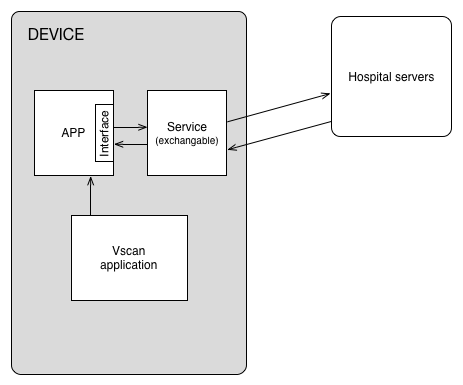
\includegraphics[scale=0.7]{img/system_arch.png}
\caption{Final system architecture}
\label{fig:overall_architecture}
\end{figure}

\newpage

%%%%%%%%%%%%%%%%%%%% NY SUBSECTION %%%%%%%%%%%%%%%%%%%%

\subsection{Architectural Significant Requirements}
Combining the requirements and business goals, the group wanted to create a secure application that was easy to use whilst reducing the cost of modifying it. While usability was important, it would not be as significant to the architecture as security and interoperability turned out to be. How the architecture reflects the functional requirements is addressed in section \ref{architectualRationale}. Table \ref{asrtable} shows the architectural significant requirements.

%Tabell for functional requirements
\begin{table}[H]

\renewcommand{\arraystretch}{1.2}
\captionof{table}{Architectural significant requirements}
\label{asrtable}
\begin{tabular}{|p{3cm}|p{9cm}|}
\hline
\textbf{FR\#} & \begin{tabular}[c]{@{}l@{}}
\textbf{Description}
\end{tabular} \\ \hline

3 & \begin{tabular}[c]{@{}l@{}}
The application need to allow doctors to authenticate\\ with the EMR-system
\end{tabular} \\ \hline

4 & \begin{tabular}[c]{@{}l@{}}
The application must be able to identify patients \\
based on SSN
\end{tabular} \\ \hline

5 & \begin{tabular}[c]{@{}l@{}}
The application need to be able to upload images to \\
the hospital servers
\end{tabular} \\ \hline

10 & \begin{tabular}[c]{@{}l@{}}
The application must not display sensitive information\\ 
if the application is in offline mode
\end{tabular} \\ \hline

12 & \begin{tabular}[c]{@{}l@{}}
The application must auto-close and/or auto-log out \\ after a  
given time interval 
\end{tabular}\\ \hline

\end{tabular}
\end{table}



\paragraph*{Interoperability}
%Having a modular product will impact on the design of the architecture.  Thearchitectural design must allow for several modules that have low couplingand high cohesion, so that it is easy and cost efective to customize one partof the system while the rest stays the same.
Interoperability is an important quality attribute for the application, as one of its main features involves communicating with an external hospital information system. 


\paragraph*{Security}
In order to properly secure the application, security has to be built in to the architecture. It is important to restrict access as well as securing resources.


%%%%%%%%%%%%%%%%%%%% NY SUBSECTION %%%%%%%%%%%%%%%%%%%%

\newpage

\subsection{Tactics}
In the following section we will describe the tactics used in order for the architecture to meet the quality requirements.

\subsubsection{Security}
\label{architecturesecurity}
Through research, it was confirmed that the back-end of the hospital information systems used a lot of security tactics, ranging from detecting attacks to recovering from them. Because of this, it was decided to focus on tactics for resisting attacks to secure the application. How this decision opens for potential threats is reflected upon in section \ref{productEval}.

\paragraph*{Authentication}
Users should provide evidence that they actually are who they claim to be. This is usually done through usernames and passwords.

\paragraph*{Encrypt data}
Data should be protected from unauthorized access. Confidentiality can be achieved by applying encryption to both data and communication.

\subsubsection{Interoperability}
The application need to communicate with a hospital information system. This is done through a service acting as an intermediary between the application and the server.

\paragraph*{Locate}
The locate tactic is about the fact that the systems involved should know about each other. 

\paragraph*{Manage interfaces}
The involved systems needs to understand each other in order to exchange information.

%The basic approach to reducing the cost of modifying responsibilities is to transform the architecture by splitting the responsibility into two portions based on the specific change to be made (Bachmann et al. 2007) \cite{1504552}.

%To accommodate for the quality attributes presented in \ref{modularityQA}, we chose to focus on increasing cohesion and reduce coupling. This, combined with carefully defining responsibility for different modules, ultimately led to the decision to separate the application into a on-device Android service and a normal GUI application, which is specified in section \ref{serviceDescription}.

%\paragraph*{Encapsulation}
%Objects should be encapsulated. The object’s functionality should be exposed to the rest of the program via its public methods.

%\paragraph*{Use an Intermediary}
%If an object depends on functionality from a complex service, an intermediary layer with a simplified interface should be used.

%\paragraph*{Restrict dependencies}
%An object should not reference other objects unless they are immediately relevant.

%\paragraph*{Split responsibility}
%Making one module of a system be responsible for a well defined task and thereby splitting the responsibility reduces the cost of particular changes.


%%%%%%%%%%%%%%%%%%%% NY SUBSECTION %%%%%%%%%%%%%%%%%%%%

\subsection{Patterns}
This section contains an overview of the architectural- and design patterns used in the application. 


\subsubsection{Singleton}
\label{singletonArc}
The \emph{singleton} pattern is a design pattern that is used in order to prohibit the instantiation of more than one instance of a class \cite{softwarearchitecture}. The idea is that instead of letting other classes access the constructor and create new instances of the class, the constructor is made private. Everything has to go through another (static) method, typically called \emph{getInstance(...)}, which handles access to the class. In the implementation, we have utilized the singleton pattern in the database helper class. Section \ref{databaseImp} will go over the implementation in greater detail.

\subsubsection{ViewHolder}
\label{viewholderArc}
The ViewHolder pattern is an Android specific design pattern used to increase performance in \emph{ListViews}. The pattern is crucial to implement when dealing with large lists to avoid bad performance. A detailed explanation of how the patterns works, as well as implementation details can be found in section \ref{viewholderImp}.


\subsubsection{MVC}
The Model-View-Controller architectural pattern (MVC) divides the architecture of an application into three components. The model contains the core functionality and data, while controllers handle user input and views display information. This pattern reduce coupling by enforcing encapsulation and makes it easier to implement an intermediary layer where needed. This ultimately makes it easier to make modifications, both to logical components as well as to the user interface. From a security perspective, the developer got more control over the data, as it resides in the model.


%%%%%%%%%%%%%%%%%%%% NY SUBSECTION %%%%%%%%%%%%%%%%%%%%


\subsection{Design Process}
In the start of the development process the group did not have access to a lot of technical information from the hospitals and their information systems. While waiting for a response, the group started the development of the user interface as this did not require much information from others than the customer. Almost all the application's functionality was already in place before the server connection was implemented.

\subsubsection{Offline Mode}
One of the additional features the customer requested was the ability to use the application without a network, or away from the hospital. This would enable the user to conduct examinations on home visits and remote locations, store all the data on the device and upload it when the application gets network access again.

The group designed offline mode to work in such a way that once network connection is lost, the application automatically enters offline mode. Here, sensitive data is stripped because it is not possible to authenticate the user while offline.

During the later part of the development period, we changed how the application decrypts the database. This change cascaded in such a way that the current implementation of offline mode stopped working. Further information about this event is found in section \ref{evaloffline}.


\subsubsection{Service}
\label{serviceDescription}

While the initial plan was to communicate with a “XML package”, the new approach included creating a separate Android Service \cite{android_service}. Research showed the code needed to do the actual communication with the hospital servers was trivial for a developer with knowledge about the system in question. However the code for connecting to one system was unique to another. This led to the conclusion that the service should be standardized in such a way that it could easily be implemented. The service should provide two tasks to the application; identifying a patient, and uploading images and examination data. An interface was defined so that developers would know what data to expect, and what to return to the application. A template for the service was also developed, and is (together with the interface) documented in the developer guide in the Appendix \ref{devmanual}.

To make this interface work, the group started working with AIDL (Android Interface Definition Language). AIDL allows the programmer to define a general interface to communicate with services without defining the exact service. This way it was possible to choose which service to use, and more services could be made later to support new standards and servers.

The content of the messages exchanged between the service and the application had to be decided. Based on information gathered from the industry, the group learned that this had to include name and SSN. In addition, Norwegian systems required department credentials in order to execute correctly (more information in section \ref{exsol}).

The application was therefore changed to support this feature, so that the technical user would be prompted with department username and password during first time set up. By prompting the user in such a way, the application also maintained a level of diversity in regards to the goal of making the application work anywhere, because the user has the option of entering his own credentials, should the hospital not operate with a department user policy.

It was early discovered that the Vscan was able to record video as well as images. The application was therefore designed with this in mind, and there is intentionally no restrictions hindering the user in uploading other files than images.

Overall, the new architecture worked exceptionally well, and also allowed for some new features. As before, when the application only was to upload data to a hospital server by a doctor, the application could now also be tailored to other medical practitioners by changing the service. This way, radiologists who did not wish to upload examinations to a shared multimedia storage, could for example be given a version where the service uploaded DICOM files to their conventional PACS.

When the service system was in place, it was decided to create an example service. Initially, the group intended to create a service that communicated with a DIPS mockup server, making it as realistic as possible. Through contacts in the industry, access to a DIPS BizTalk server in Oslo was acquired. We encountered several, both technical and practical, problems when trying to implement this service using the HL7 CDA R2 messaging standard. Because these issues were not resolved, we have not included the design and implementation details of the DIPS service in this report. However, these details can be found in Appendix \ref{biztalk}. 

As a backup plan we designed a really simple service, just to illustrate that our architecture worked. This service would query an SQL server for patient data, and uploading the image data to an SFTP server. This service was quickly implemented, and it communicated with the application as intended.

\noindent
Because Vscan Gateway, described in section \ref{vscan} of the report, was able to generate an examination report as a PDF, the group decided that the backup service should do the same. To build further on the proof of concept, the service never stores any data to disk, including the PDF which is generated in memory. An example report generated by the backup service, can be found in Appendix \ref{dummyServiceReport}.


\subsubsection{Settings}
The choice to use an XML file to setup the application was one of the first features that was implemented, and never actually changed. The reason for this is that it would make it easier for technical users to set up several devices at the same time, as well as providing the rest of the system a modifiable list of settings that could be expanded as more parameters were needed. The XML parser was originally implemented to work with both the package system and the settings. When the package system idea was scrapped, only the settings utilized the parser.


%%%%%%%%%%%%%%%%%%%% NY SUBSECTION %%%%%%%%%%%%%%%%%%%%


\subsection{Architectural views}
We considered the developer and the customer to be the two stakeholders that had to understand the structure of the application. Based on this, a development view and process view were created to help these groups of stakeholders get an understanding of the application.

%In order to achieve this, a component and connector view and a allocation view were created for making stakeholders understand the concepts  

\newpage

\subsubsection{Development view}
The development view illustrates the system from a developers perspective \cite{softwarearchitecture}. The emphasis is on the layers the system consists of, and serves the purpose of giving developers of getting an overview of the system. A three-layer structure is used in order to separate the key parts of the application. These are the graphical user interface, the application logic, the service and the underlying operating system (Android SDK).

\begin{figure}[H]
\centering
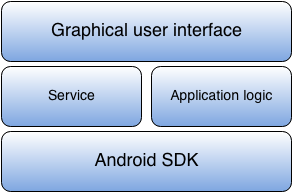
\includegraphics[scale=0.7]{img/development_view.png}
\caption{Development view}
\label{fig:development_view}
\end{figure}


\subsubsection{Process view}
The process view focuses on representing the flow of the application in a way that is easily understandable for all the stakeholders. It shows how the application combine different actions into a seamless process. As the application starts, the user has to make a decision. This happens with the "Login"-view, and there are three possible outcomes: either the user is able to authenticate to the hospital server, or the application in offline mode, where all existing data is anonymized. The only possible operation in this mode is to add new examinations or view the images of old ones. The third possible entry point is as a technical user. This option is protected by a password. The rest of the process is illustrated in the flowchart below.

%Deprecated!
\begin{sidewaysfigure}
    \centering
    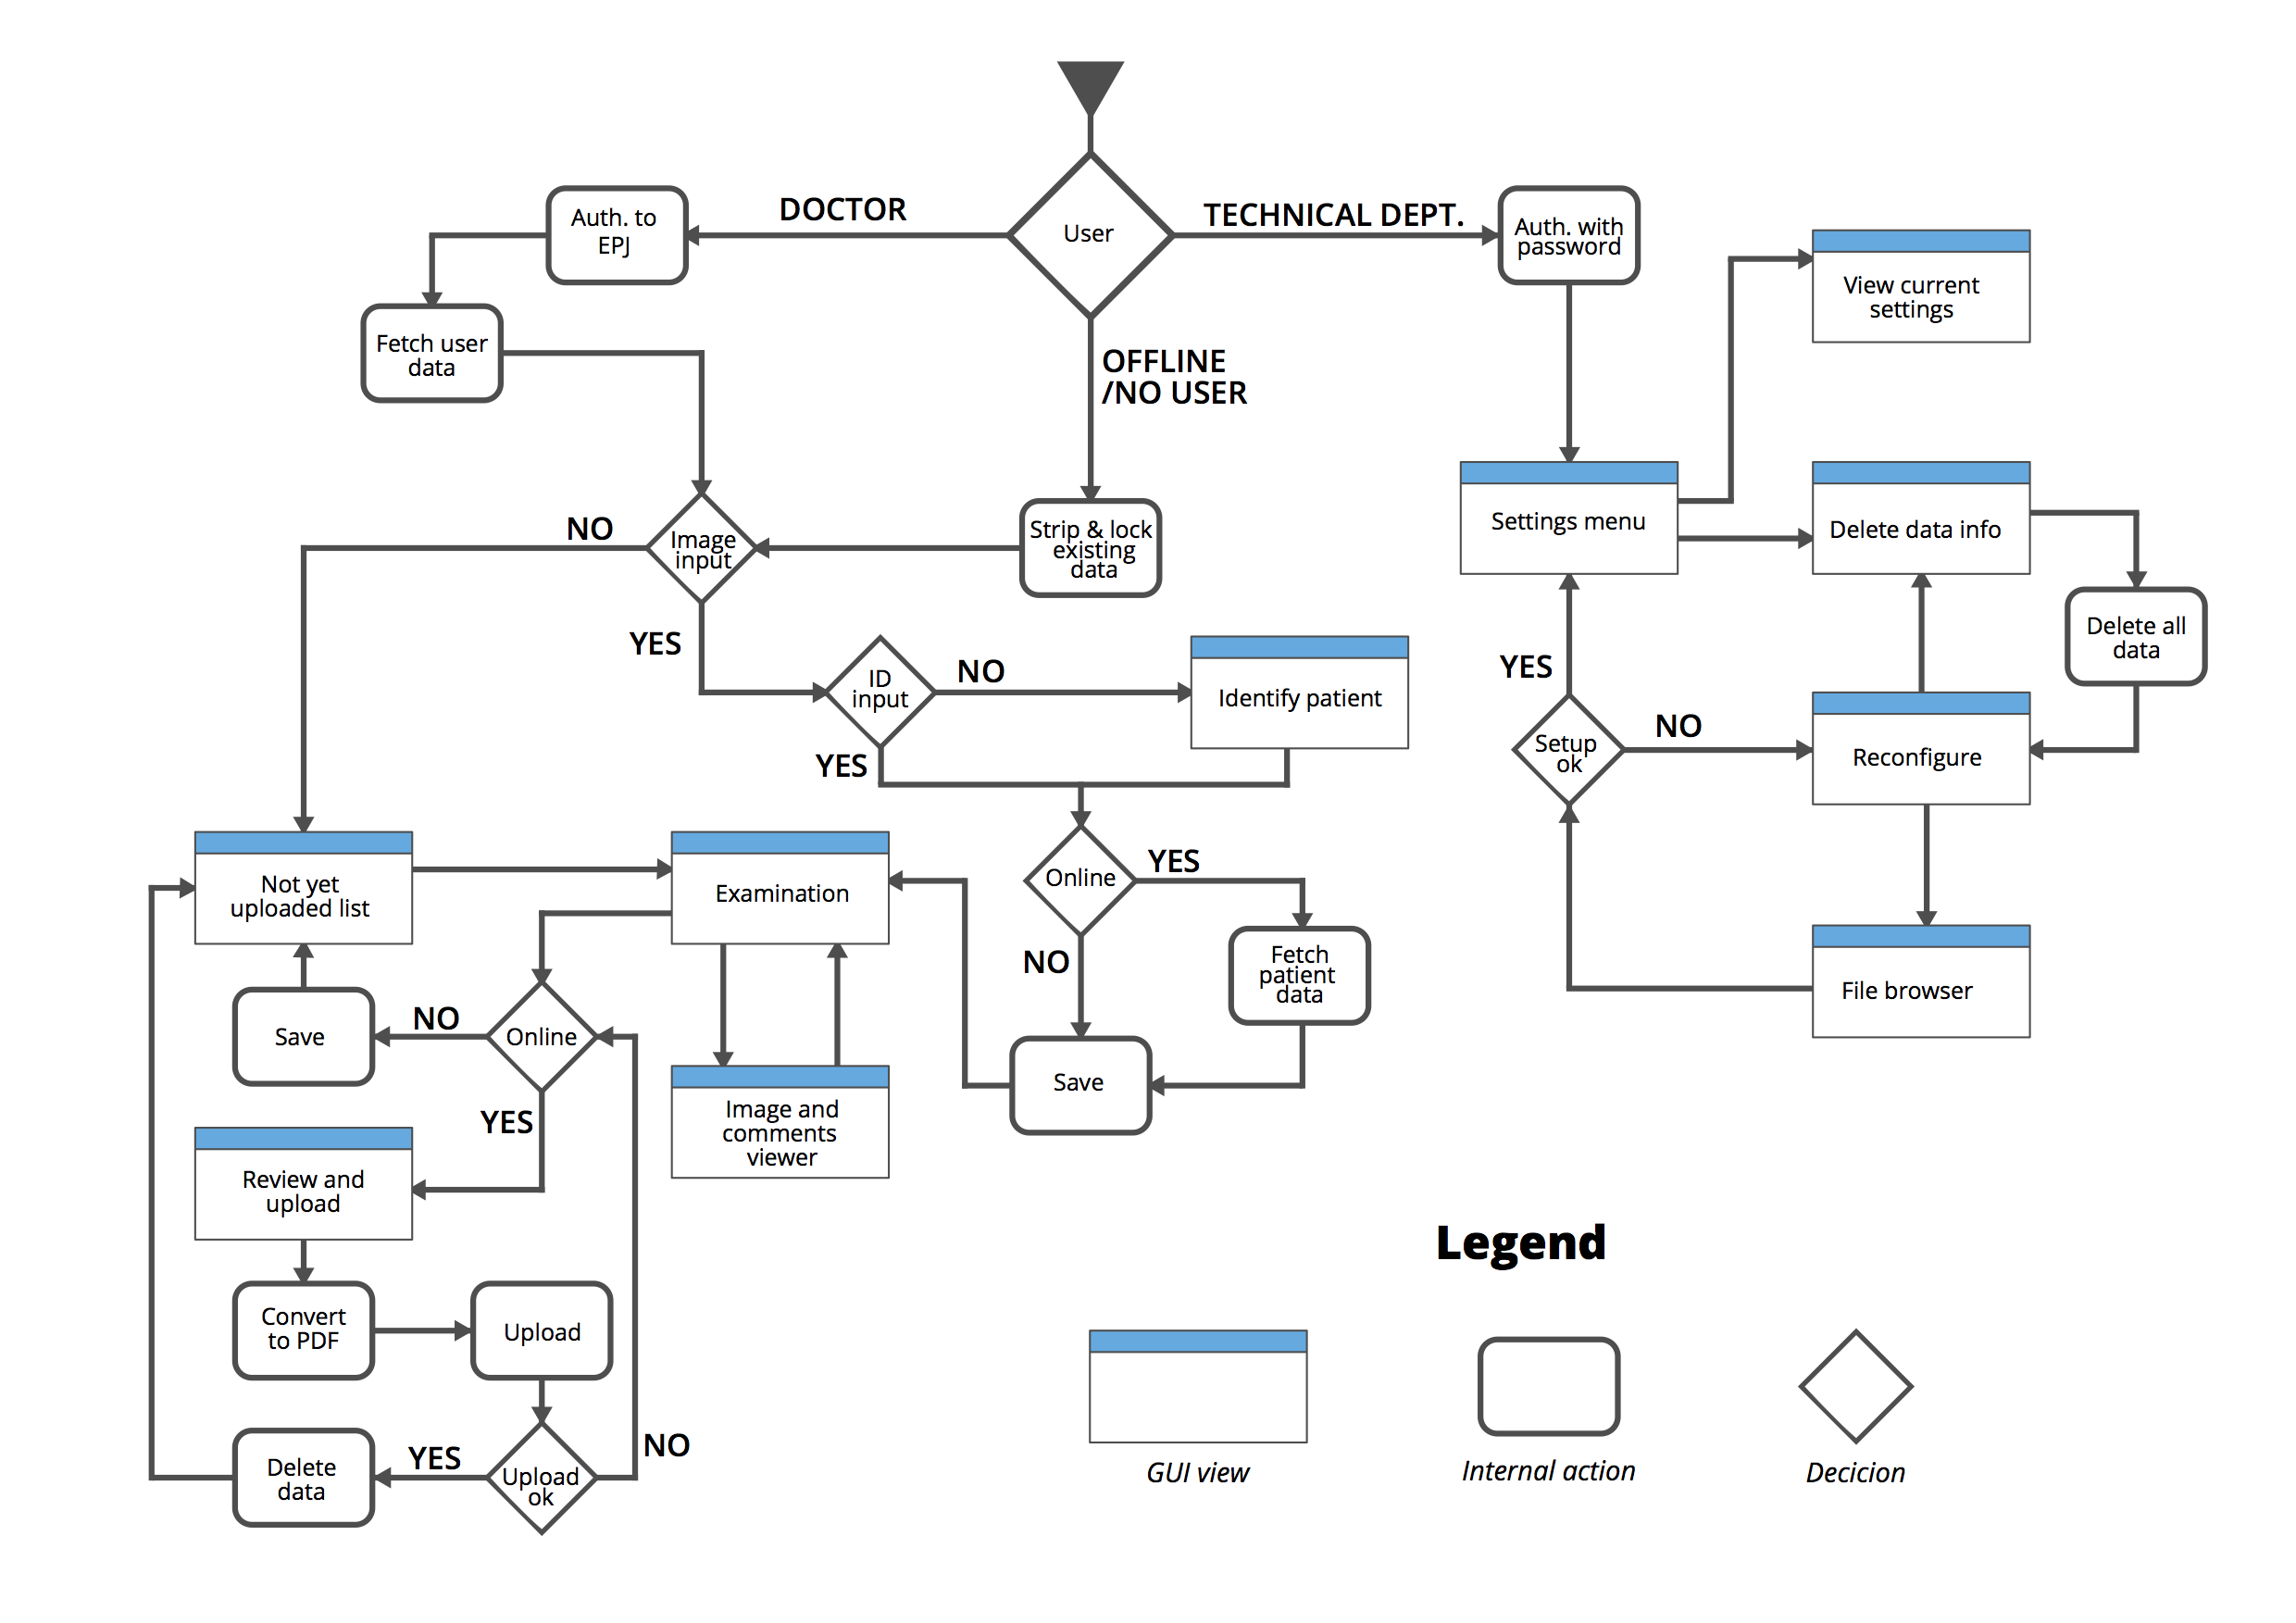
\includegraphics[scale=0.45]{img/flowchart.png}
    \caption{Process view of the application}
    \label{fig:flowchart}
\end{sidewaysfigure}
\newpage


%%%%%%%%%%%%%%%%%%%% NY SUBSECTION %%%%%%%%%%%%%%%%%%%%


\subsection{Architectural Rationale}
\label{architectualRationale}
The functional requirements and quality requirements are designed to reflect the architectural drivers and the interests of the stakeholders. In this section, how the architecture fulfills these requirements will be described.

\subsubsection{Functional Requirements}
First of all, the application needs to allow doctors to authenticate to the hospital servers. This is fulfilled by using Active Directory as an authentication service.

The functional requirement describing how the application must be able to identify patients based on SSN, is fulfilled by sending the information to the Android service. This takes care of communication with the respective hospital system.

To fulfill the requirement about being able to upload images to the hospital servers the application lets the Android service take care of this too.

\subsubsection{Quality Requirements}

\paragraph*{INT1 \& INT2 - Different services, same functionality}
By separating the architecture into one application and one service, we fulfilled both of the interoperability requirements. Through the AIDL interface, it is possible to implement new versions of the service. By replacing the service the same application can communicate with different hospital systems. At the same time this enables the main application to stay the same regardless of what service is actually used.

\paragraph*{SEC1 - Encrypted data}
The application fulfills the quality requirement regarding encrypted data with the use of SQLCipher - encrypting the database. This is done by encrypting the whole database file, and no additional concerns regarding architecture was needed.

\paragraph*{SEC2 - Data should not be able to leave the application}
With the model-view-controller approach, we got better control of the the data as it resides in the model instead of being scattered around.
\section{Implementation}

This chapter will cover the implementation process as well as a detailed description of the final implementation of the application.

\subsection{Introduction}

The main application consists of different views, extending the Android Activity class, and several helper and model classes. All examination data is stored in an SQLite database, and can be presented as individual examinations using the \emph{Examination} model class. The application uses an AIDL to communicate with a service specified in the application settings. This service is made for each hospital to account for the difference in standards and servers used.

\subsubsection*{Android Development Terminology}
This section will cover a few terms used in this document for readers unfamiliar with the Android development platform.

An \emph{Activity} is defined as a single, focused thing that the user can do. Almost all activities interact with the user in some way, and are in most cases a single view with UI elements. To start activities and services an \emph{Intent} is used. The \emph{Intent} is an abstract description of an operation to be preformed, and works as a passive data structure to transport data between different activities.

The application \emph{Context} is an interface to global information about the application environment. This is used to access the same SharedPreferences from different activities within the application. \emph{SharedPreferences} is a local storage space offered by the Android operating system where \emph{key, value pairs} of primitive data types can be permanently stored.

A Service is a component that runs without any user interaction, and is designed to do long-running operations in the background. A \emph{ServiceConnection} is used to communicate with the service. To start using a service, the \emph{bindService()} method is called. If the service is bound successfully, it will return an \emph{IBinder} object that can be used to communicate with the service.

AIDL (Android Interface Definition Language) is an interface language used to define general interface structures for service communication. It is used to communicate with services outside of the application itself. When the \emph{.aidl} file is compiled for Java, it will create a Java interface class that will act as a service.

\subsection{Implementation Details}

This section will describe how the different parts of the application were implemented and how the different modules interact with each other. A complete overview of the different packages and their relation can be found in the Appendix \ref{classdiagram}.

\subsubsection{Initial Setup}

Before the application can be used, it has to be configured to work with the correct hospital. As the application itself is dependent on several settings that the normal user not necessarily will have access to, it is required that the application is set up by technical personnel before use. These settings range from hospital server addresses, to department credentials and authentication variables.

Figure \ref{fig:config} illustrates the scenario where the technical user starts the application for the first time, sets a password for restricted access to the "Settings"-view, and configures the application with a preconfigured settings file. This file is downloaded from a hospital HTTP server.  

\begin{figure}[H]
\centering
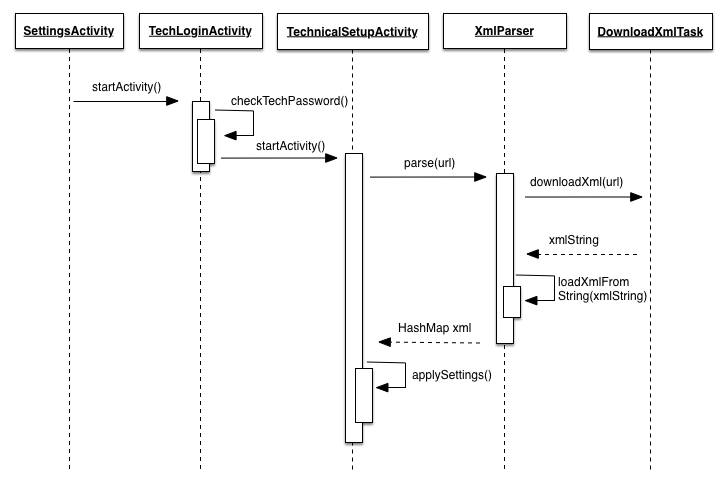
\includegraphics[scale=0.5]{img/sequence_config.png}
\caption{First time configuration}
\label{fig:config}
\end{figure}

\subsubsection{User Interface}
\label{viewholderImp} 

After the initial setup, the only way to start the application is through the Vscan application. As the Vscan application was not a part of the project, the \emph{GatewayLauncher} class was created as a template for launching the application.

The "Login"-view is the first view presented to the user no matter which launcher method is used, and the \emph{LoginActivity.java} will redirect the user to different parts of the application, depending on the information from the launcher. The most important part of the launcher is the first four static variables. These variables tells the LoginActivity which part of the application to start. The different constructors are there to ensure that the correct information is provided for the different launch modes. More information about the different launch modes will be covered in section \ref{appworkflow}.

To implement MVC we used an \emph{Examination} class as the model for each examination. The \emph{ExaminationActivity} is both view and controller for this model while \emph{HomeScreenActivity} and \emph{ReviewAndUploadActivity} only serves as views. The second model is the \emph{EMRApplication} class, which holds all application settings. \emph{CurrentSetupActivity} is used to view this model, and \emph{TechnicalSetupActivity} is used as a controller.

For showing data in a scrollable list, a \emph{ListView} is used. A ListView is, like the name suggests, a view group of elements that together constitutes a list. A ListView can contain any number of elements. In Android, an \emph{Adapter} acts as a bridge between the ListView and the data it displays. Figure 16 shows the relationship between the adapter, underlying data and an activity. When an user scrolls the ListView, the adapter's \emph{getView(...)} method is called. This method will repeatedly call \emph{findViewById(...)}, which retrieves layout widgets in the UI. The \emph{getView}-method will then return a View and tell the ListView to display it. This happens for every row visible on the screen as well as the next and previous rows to be shown \cite{adapter}. When dealing with a large amount of data, this may cause scrolling ListViews to be slow and choppy due to the \emph{findViewById(...)}-method being called repeatedly. This is where the ViewHolder pattern comes in \cite{viewholder}. The ViewHolder is told to hold the layout widgets so they don't have to be retrieved time after time with the \emph{findViewById(...)}-method. Listing \ref{lst:viewholder} shows the implementation of ViewHolder pattern in \emph{ReviewListAdapter.java}.

\newpage

\begin{lstlisting}[caption={ViewHolder implementation}, label={lst:viewholder}]
// ReviewListAdapter.java
private LayoutInflater inflater;

static class ViewHolder {
    TextView imageDateTextView ;
    TextView commentTextView;
    ImageView rowImage;
}

@Override
public View getView(int position, View convertView, ViewGroup parent) {

    ViewHolder holder;

    if (convertView == null) {
        convertView = inflater.inflate(resource, null);

        holder = new ViewHolder();
        holder.imageDateTextView = (TextView) convertView.findViewById(R.id.imageDate);

        convertView.setTag(holder);
    } else {
        holder = (ViewHolder) convertView.getTag();
    }
    return convertView;
    }
}
\end{lstlisting}

\noindent
The call to \emph{findViewById()} happens at line 21, and the ViewHolder is told to hold the \emph{TextView}. The next time \emph{getView()} is called, the method will not have to call \emph{findViewById()}. This will greatly improve performance, especially with large lists.

\begin{figure}[H]
        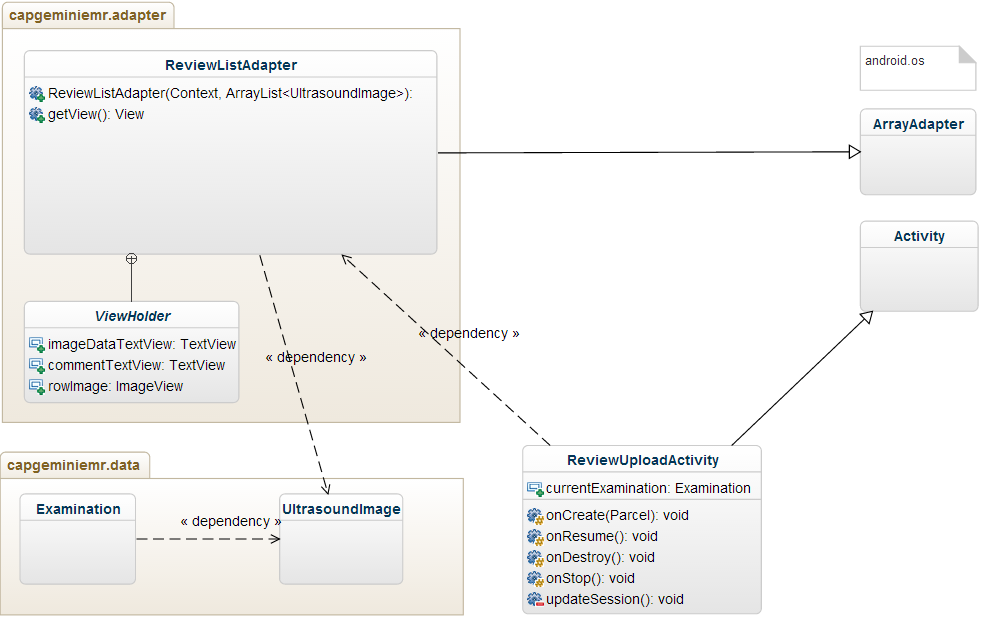
\includegraphics[scale=0.5]{img/classdiagram2.png}
        \caption{Relationship ListAdapter, data and Activity}
    \label{classdiagram_data_adapter}
\end{figure}


\paragraph{Application workflow}
\label{appworkflow}

Disregarding the technical views, the application is designed to have a very linear flow, where the user is guided step-by-step through the process of preparing and uploading the examination. As the application itself is only reachable through the Vscan application, there are three different ways for the application to behave. 

In the first scenario, the user only wishes to identify the patient prior to an examination. Given this scenario, the application launches, the user logs in and inputs or scans the patients SSN. If the SSN is recognized, the application returns the patient information back to the Vscan application, and the application finishes. 

In the second scenario, the user wishes to conduct and upload an examination. Data from the examination is used to launch the application. Dependent upon if the scenario above has taken place, the user either inputs (or scans) the patient's SSN, or the application automatically utilizes the information retrieved from the first scenario. The user then arrives at the "Examination"-view, where he is given an overview over the patient's information, and is given the option to add a comment on the examination as a whole, as well as the option to review the images. By choosing to review the images from the examination, a full screen view of the images are presented to the user, where the user can zoom in on images for further inspection, swipe between them, delete images not to be uploaded, and add comments to each image. When the user is done, the full screen view can be closed by clicking the "close"-button, which returns the user to the "Examination"-view. 

The "Examination"-view informs the user of the number of images lacking a comment. This is a part of the design feature, intended to ensure that all images uploaded by the user, is of diagnostic value, mentioned in section \ref{multimediaInHospitals}.

When done, the "Review and Upload"-button takes the user to the view with the same name. The view is designed with the same intention as above, forcing the user to scroll through each image of the examination. At the bottom of the list, the user is presented with the option to either edit the examination, taking the user back to the "Examination"- view, or to upload the examination. If the user chooses the latter option, a dialog will alert the user if any images lacks comments. 
After the potential dialog has been disregarded, the process of uploading the examination is initiated. After completion, the user is returned to the "Not yet Uploaded"- view (described in details bellow).

In the third scenario, the user wishes to view stored examinations. After login, the user is sent to the "Not yet Uploaded"-view, where all examinations are listed. The user here has the option to either delete or upload the examinations. 

Common to the scenarios above, is that if the application for any reason detects either network loss or session timeout, all sensitive data is stripped from the views. The user is still able to enter sensitive data, but is not able to see information already entered.


\subsubsection{Database}
\label{databaseImp}

The need for a local database is mainly rooted in the fact that the application should be working offline. Additionally, having progress be stored at key points in the application flow ensures that work is never lost should the application unexpectedly close or be terminated after these key points. As mentioned earlier, the database is encrypted because it contains sensitive data. This may lead to a performance problem, especially on older and slower devices.

Figure \ref{fig:database_design} shows the database design. It consists of two tables; \emph{Examination} and \emph{UltrasoundImage}. An \emph{Examination} has one or more \emph{UltrasoundImages}, each with a comment and an image URI pointing to where the image is stored on the device's SD-card. The \emph{Examination} entity reflects the Examination class presented in in regards to MVC in the previous section. \emph{UltrasoundImage} is linked to \emph{Examination} with the Examination's id as foreign key.

\begin{figure}[H]
\centerline{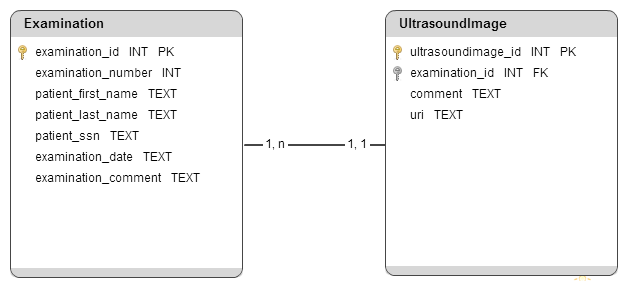
\includegraphics[scale=0.9]{img/database_design.png}}
\caption{Database design}
\label{fig:database_design}
\end{figure}

\noindent
Everything related to access to the database is handled by a class named \emph{DatabaseHelper.java}. The relationship between the database helper class and the data model classes is shown in Figure 18. DatabaseHelper has methods for adding, deleting, updating and retrieving \emph{Examinations} to/from the database. A point worth noting is that the data classes Examination and UltrasoundImage both implements \emph{Parcelable}. Parcelable allows for object instances to be written to and restored from a \emph{Parcel} \cite{parcelable}. This makes it possible to pass object instances from one activity to another via Intents without having to depend on temporary storage in the database. 

\begin{sidewaysfigure}
    \centering
    \label{fig:classdiagram_db_data}
        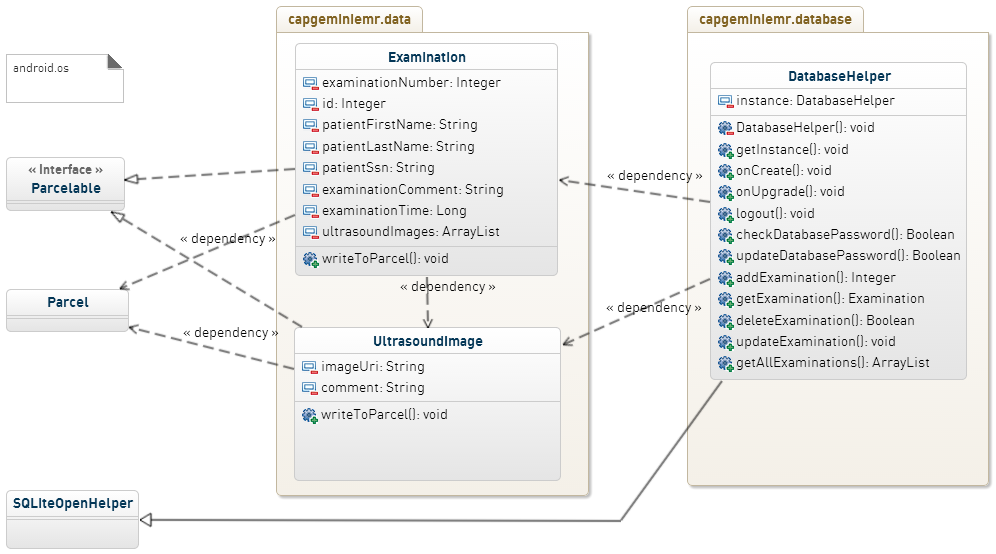
\includegraphics[scale=0.75]{img/classdiagram1.png}
        \caption{Class diagram: database and data}
\end{sidewaysfigure}


\newpage
\noindent
The DatabaseHelper class is used by multiple activities. In order to keep only one instance of this class that may be used throughout the application, we have implemented a \emph{singleton pattern}. Listing \ref{lst:database} shows the implementation of the singleton in \emph{DatabaseHelper.java}.

\begin{lstlisting}[caption={Singleton implementation}, label={lst:database}]
// DatabaseHelper.java
private static DatabaseHelper instance = null;

private DatabaseHelper(Context con, ArrayList<String> databaseInfo) {

        super(con, databaseInfo.get(0), null, DATABASE_VERSION);
        this.password = databaseInfo.get(1);
}

public static synchronized DatabaseHelper getInstance(
  Context con, ArrayList<String> databaseInfo) {

    if(instance == null) {
        SQLiteDatabase.loadLibs(con);
        instance = new DatabaseHelper(con, databaseInfo);
    }
    return instance;
}
\end{lstlisting}

\noindent
As described in section \ref{singletonArc}, the idea behind a singleton is that instead of letting other classes directly access the constructor and create new instances of the class, everything goes through a public method called \emph{getInstance(...)}. The constructor is therefore made private. The singleton class stores an instance of itself in a private field (appropriately named \emph{instance}). Every time some other class needs a \emph{DatabaseHelper}, they simply call the static method \emph{getInstance(...)} of DatabaseHelper instead of calling the constructor. This method will create a new instance of DatabaseHelper if the private field \emph{instance} is null and then return it. If not, it will return the existing instance instead of creating a new.

The reasoning behind using a singleton for the database helper is for performance reasons and the fact that no more than exactly one instance of the class will ever be needed. Performance is increased because the static method \emph{loadLibs(context)} of the SQLite database is an ''expensive'' operation when using SQLCipher and should therefore not be called more than needed.

\paragraph{Encryption}
The system uses two different encryption methods. To encrypt the database, the open source extension to SQLite called SQLCipher is used. To encrypt the password used to authenticate users, the cryptology package in Java is used. SQLCipher uses 256-bit AES (Advanced Encryption Standard) to encrypt all the database files. The Java cryptology implementation uses 128-bit AES encryption.

\subsubsection{Settings}

All necessary settings will be supplied to the application through an XML file containing all information needed for communication with external systems. This file is required to use the application. The first time the application is launched, the technical user will be prompted to enter the technical password to protect the technical part of the application. The layout of the XML file, as well as more in depth instructions for how to set up the application can be found in the technical manual (Appendix \ref{techmanual}). Once this password has been set, the user is required to supply an XML file containing all the communication settings for the application. The application will then parse the file, and save the settings to the \emph{SharedPreferences} of the application. The advantage of this is that non-sensitive data can be stored persistent, even when the application is closed or the device restarted.

A list of current settings can be found by choosing "View current settings" in the "Settings"-view. The technical password is required to access this page. To change the settings the user can choose to reconfigure the application. This will also require the technical password, and the user can once again supply an XML file with the new settings.

\subsubsection{Authentication and Session management}
\label{sessionimplement}
The application uses LDAP to authenticate users. All information needed to connect to the correct authentication server is supplied in the application settings. 
\noindent
LDAP is an application protocol used to query and modify items in directory services such as Active Directory. The application supports regular LDAP as well as LDAPS (LDAP over SSL). The process is described in Figure \ref{fig:login}.

\begin{figure}[H]
\centering
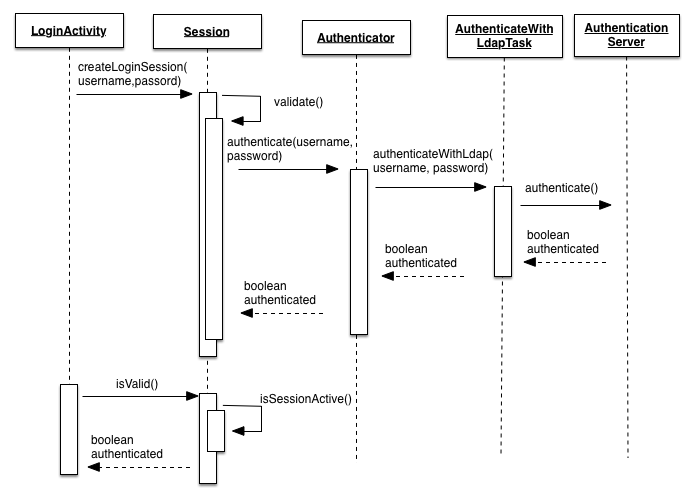
\includegraphics[scale=0.5]{img/sequence_auth.png}
\caption{Login}
\label{fig:login}
\end{figure}

\noindent
Even though LDAP was the only method implemented during this project, the application is designed to allow for the implementation of other authentication methods (such as Kerberos \cite{kerberos}) in the future.

To allow the user to easily switch between the application and the Vscan application, a session based system was designed. On a successful authentication a new session will be created. The session will store the username and a password hash to SharedPreferences and create a time stamp set to 10 minutes in the future. 

Every time the user navigates between activities in the application, a method in the session class will be called to check if the session is still valid, comparing the time stamp to the current time. This method will also check network connectivity, as a login session will not be valid if the user has lost connection. If the session is still valid, the time stamp will be updated. This way, the session will always be valid 10 minutes after the last interaction.

\subsubsection{AIDL and Services}

The AIDL interface is defined in a file with an \emph{.aidl} file extension. This file is supplied to both the application and the service. It is important that the file is in the exact same package on both ends. The service can then implement the Java interface generated by the AIDL file.

The application can use a method in the compiled AIDL file called \emph{Stub} to access the service interface. Before binding to a service, a new Intent is created, and its \emph{setClassName()} method is called with a reference to the package of the AIDL file and a reference to the actual service, both defined in the application settings. This intent is then supplied together with the actual Java interface to bind the service.

The final implementation of the AIDL interface consisted of two methods; one of them, identify patient method, would take in a SSN or similar identification numbers as a string, and return a list of information based on that number. The other function, upload images method, would take in three lists, one with patient information, one with images and one with comments to the examination and images. This method would return a Boolean variable reporting the success of the upload. Both methods also has a username field and a password field for communication with the hospital servers.
\begin{lstlisting}[caption={AIDL Interface}, label={lst:finalaidlinterface}]
// EMRRemoteInterface.aidl
package org.royrvik.emrservice;

interface EMRRemoteInterface {
    List<String> getPatientData(in String ssn, in String username, in String password);
    List<String> upload(in List<String> examinationData, in List<String> imagePaths, in List<String> notes, in String username, in String password);
}
\end{lstlisting}
\smallskip
The identify patient method was designed to hold the patient's SSN, while the return message would contain an array with the patient's first name and last name. The messages could however be easily modified, should the customer wish for additional data.

The upload images method is more complex, and contains three arrays; examination data, images and notes. Examination data contains all data from the examination, as well as the patient information, all in a well defined format (see Appendix \ref{devmanual}).
Images contains the path to the images, and notes contains the notes to each image.
\noindent
The response messages for both tasks is structured as an array. In addition to response data (i.e first name), the message contains a boolean \emph{didWork} together with an error message. Figure \ref{fig:service} describes the process for acquiring patient data, as well as uploading an examination for any service created for the application.   

\begin{figure}[H]
\centering
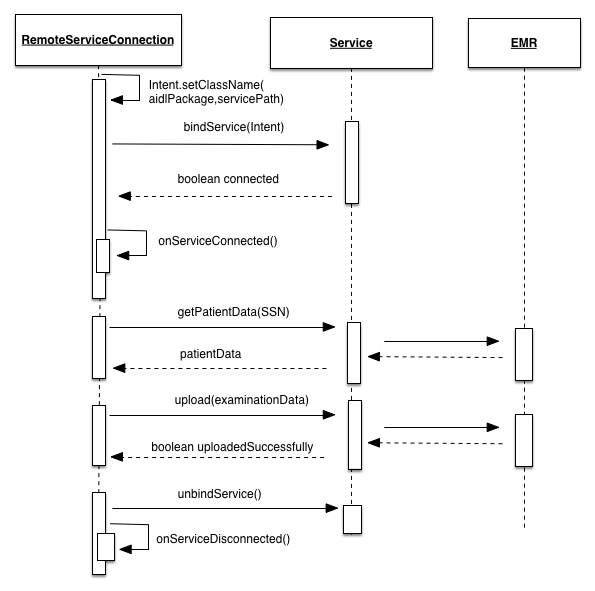
\includegraphics[scale=0.5]{img/sequence_service.png}
\caption{Application/Service communication}
\label{fig:service}
\end{figure}


\subsubsection{Offline Mode}
The offline mode functionality was implemented half way through the development process. This would strip all sensitive data from the application, while still enabling the user to edit the fields and view the images.
\noindent
At the end of the development process the database security was changed to use user credentials to encrypt the data instead of a static key. This caused the offline mode feature to lose database access when the user was unable to log in. The stripping functionality remained in the application, but the offline mode functionality itself was never implemented with the new database. 
\noindent
The group felt that a secure database was more important than a working offline mode, and prioritized more important parts of the application.

\subsubsection{Security}
As one of the projects quality attributes was security, the group spent a good amount of time figuring out how to secure the data storage. The techniques and tactics we used can be found in section \ref{architecturesecurity}. In the following section we will discuss how these tactics were implemented.

\paragraph*{Storage}
One of the biggest security issues of the project, was to store patient data safely on the device. As described in the architecture chapter, the choice fell on encrypting the database. The library used to encrypt the database file ensures that the file is encrypted at all times, which entails that the database remains secure even if the application should crash. Although implementing the encryption functionality was rather straight forward, figuring out how to handle the encryption key was a bigger struggle. It would of course defeat the purpose to have the encryption key in a code variable, and storing it elsewhere on the device was found to be unsafe. 

Storing it as a hash in Android's SharedPreferences was considered, since an application's SharedPreferences is restricted only to the application itself through UNIX permissions. This was quickly dismissed since research show that a rooted device, and its applications, would easily have its SharedPreferences compromised if an attacker wanted said information. Even if the encryption key was to be hashed, this would most likely only slow down the attacker. 

\noindent
Although the obvious and ideal solution to this problem is to have the encryption key as user input, but having users input a shared decryption key in addition to their own credentials was dismissed as unintuitive, impractical and unsafe. This would in addition put a lot of extra constrains on the user, which we - as stated in the USA5 quality attribute - wanted to avoid. 

The solution to this problem was to give each user their own database, where each database used the individual users password as encryption key. To know which database belonged to which user, it was decided that the name of each database file was the username of the user ("username".db). This also added a new feature to the application, as it is an industry practice to restrict the level of access medical personnel has after the “Not more than needed”  principle. Although this solution solved the main problem of safe storage, it also brought with it issues in regards to password policy. The application had to be able to handle a user password change, which happens frequently; once every third month at the hospitals the group had been talking to.

The application was now designed to have an encrypted database file for each user. If a new user was to log in, the application would detect this because no database with the name of the users username existed. In the same way the application would be able to determine if a user had changed his password, because he would be able to authenticate with the hospital servers (currently through LDAP), but not be able to decrypt the database. Functionality was therefore implemented to prompt for the users previous password to change the encryption key.

The implementation is not an optimal one, as it requires the user to remember both old and new password, but it was still chosen as the best solution by the group. A good argument for this solution, is that the workflow is structured so that an examination is to be uploaded within a reasonable time after it has taken place. If a password is still changed before the user has had time to upload the examination, it should still be fresh enough in his or her memory to not be a problem. If the user cannot remember his old password, the database can be deleted, so that a new database (with the new password) can be created. 


\subsubsection{Other Safety Measures}
Despite the safety measures described above in the security section, there were some worries related to the settings functionality. Given that an attacker somehow was able to steal a device, and put it back afterwards, the attacker could either switch the current service with a malicious service, and change the configuration so that the application sent sensitive data to that service. It was also a worry that the settings could be tempered with to such a degree, that data credentials could be sent to a malicious server. 
To counter this, it was determined that the technical user would set a password on the settings view so that no other then technician would be able to reconfigure the application. The settings file was changed to specify the name of the service, and an the settings view was changed so that any editing of the application settings would cause the entire database to be wiped.
According to the SEC2 requirement, no non-encrypted data should \emph{escape} the application, and be saved to disk. To fulfill this we have disabled the possibility to take screenshots while inside the application. Listing \ref{lst:disablescreenshot} shows how this was implemented.
\newpage
\begin{lstlisting}[caption={Screenshot disabling}, label={lst:disablescreenshot}]
getWindow().setFlags(WindowManager.LayoutParams.FLAG_SECURE, WindowManager.LayoutParams.FLAG_SECURE);
\end{lstlisting}



\subsection{User Manuals}

The group decided to divide the users into three user groups; 
\begin{itemize}
    \item Service developers 
    \item Technical staff
    \item Regular users 
\end{itemize}
This was done because a doctor (considered a regular user) should not need to know how the application works or the address and protocols for every connected server. Neither should technical staff at the hospital be required to know programming well enough to develop the service themselves.
The service development guide can be found in Appendix \ref{devmanual}. Technical manual is located in Appendix \ref{techmanual}, and user manual can be found in Appendix \ref{usermanual}.

\newpage
\subsection{Sprint summaries}
In the this section we will give a brief overview of our development process. Each week was documented by a weekly report. An example can be found in Appendix \ref{weekly_rep}.

\subsubsection{Sprint 1}
The group spent most of its time getting familiar with the task it was assigned, and furthermore how to approach the task in terms of work methodology. A draft of the projects requirements was developed, and the process of establishing a network of contacts from the industry was initiated. 
    
\subsubsection{Sprint 2}
In the beginning of this sprint, the initial requirements were in place. An architectural draft of the application was completed, and mockups of the GUI was finalized, tested and implemented. In regards to research, the group experienced a steep learning curve on the amount of systems used at hospitals. PACS, DICOM and how to communicate with hospital servers was the main focus as the group acquired contact in both OUS, DIPS and The Norwegian Directorate of Health. 


\subsubsection{Sprint 3}
The main focus of this sprint was research and implementing offline-mode functionality. The group also spent time to figure out how to actually communicate with different hospital information systems, and which protocols that needed to be used. During this process, a lot of emails were exchanged with contacts we had established with the industry.

During this sprint's research, the group was made aware that not all medical personnel can use PACS for storing images. Since this was the system the customer initially had suggested that the images should be uploaded to, further research into other systems was needed.

\subsubsection{Sprint 4}
\label{sprint4}
At this stage, the group realized that rules and regulations as of today prevented us from uploading images from mobile devices to a hospital information system (see \ref{multimediaInHospitals}). Nevertheless, together with the customer we decided to ignore this, and focus our work on figuring out how to upload data to the PAS/EMR, just as a proof of concept. Alongside with this, the customer also wanted us to explore future solutions in greater depth.

In parallel with the research that was done, a lot of the applications core functionality was implemented. This included the SQLite database, settings, authentication, sessions and QR code scanning.   


\subsubsection{Sprint 5}
In sprint 5 the final architecture of the service was designed. Building on the new architecture, the group worked on creating a service that would communicate with a DIPS BizTalk server, given to us by Sykehuspartner. This was intended to be a dummy DIPS service, illustrating the functionality of the new service implementation.

BizTalk technology required communication to happen through C\#. The group had to do research both on the Windows Communication Framework/.NET, as well as how to make C\# code run on Android.

Because of technical issues with the DIPS server, a simple backup service using MySQL and SFTP was developed instead. During this sprint a lot of security features were also added, including database encryption.    


\subsubsection{Sprint 6}
This sprint was used to complete the development process, as well as producing a first draft of the final report. 

During the sprint, the backup service was completed and the communication between the application and the service was standardized and documented. The user interface went through a complete overhaul, giving it a clean look and feel. A new "Full Screen Image"- view was also implemented, making it easier to view and comment on images. In addition to this, a lot of time went into fixing known errors and bugs.
\section{Testing}
In this chapter we will describe how the testing process has been conducted and present its results. The test plan is derived and developed from the Standard for Software Test Documentation (IEEE 829-1998) \cite{iee829}. Items from the standard that the group did not consider necessary are not included in the report.

\subsection{Introduction}
This section will cover any background information, general testing strategy as well as definitions and acronyms used specifically in this chapter and related documents in the Appendix.

\subsubsection{Objectives}
When the group had a working implementation of a module with the basic functionality, all the related tests were ran to ensure that the module worked as intended. The test plan was updated for each report delivery. When a sprint introduced new requirements or features, the test plan was updated during or after that particular sprint. The major work activities related to the test plan was the initial writing of the document itself, generating the test items and finally executing the tests.

\subsubsection{Testing Strategy}
The tests described in this document were executed on the final product to uncover hidden bugs or errors and ensure that everything was working as expected. Tests for each module was also used during the development process to ensure that the module was implemented correctly. No testing frameworks were used in the testing process because the group did not have any experience with automatic tests, and did not have time to learn it during the project.

\subsubsection{Scope}
The Test Case was updated as new components and features needed testing, and most of the tests became a requirement for the implementation itself. The Test Plan only had one big rewrite between the mid-term and the final report.

\subsubsection{Reference Material}
Individual tests and test items are listed in the Test Case document, Appendix \ref{testdoc}. The requirements for each of the test items are referencing the requirements in report chapter \ref{requirements}.

\subsubsection{Definitions and Acronyms}
The names for each test item is composed of a prefix to indicate what part of the system the item is from, followed by an underscore and an incremental ID for each prefix: e.g. UI\textunderscore0003 will be the third test item from the User Interface part of the system.

Full list of prefixes and their relation:
\begin{itemize}
\item UI  	   	- User interface
\item SYS  		- General system requirements
\item NET 		- Communication with other systems
\item SEC 		- Security requirements

\end{itemize}

\subsection{Features to be tested}
All modules listed in the test case document, Appendix \ref{testitems} were tested. This includes all user interface components, general application workflow, service communication and basic security measures.

\subsection{Features not to be tested}
Android platform specific security was not tested, as it goes beyond the scope of this project. 

The QR code feature, requirement 6, will not be tested, as this is a separate application and will only be used to type in the patient SSN faster.

Requirement 10, stripping of data in offline mode, was not tested as this was a feature the group determined it was a feature that was no longer needed. This is covered further in the evaluation, chapter \ref{evaloffline}.

\noindent
Because of time constraints, a complete acceptance test of the final application was not conducted. An informal test with an end user was however performed (see section \ref{acceptance_test}). In addition to this test, the final product was presented and approved by the customer.

\subsection{Approach}
This section describes how the group conducted the different types of tests.

\subsubsection{Component Testing}
Each component of the system was tested manually during development, and the group as a whole worked together to uncover more bugs on the finished implementation of each module. This was quite easy and effective, as the product do not require every part of the system to work correctly in order to run. Because none of the group members had any experience with automated test frameworks and testability was not a success criteria, we did not take use of this.

To ensure that the finished product worked as expected, the group also ran all the tests described in the Test Case document at the end of the development process. 

\subsubsection{Interface Testing}

After the first round of GUI mockups was finished, an usability test was done with a small group of students to test if the UI was intuitive and user friendly. The final implementation and design did differ a bit from the original mockups, but mainly this was not due to the results from the usability test. The reason we modified it was because the look and feel of the implemented versions of the mockups, did not comply with what we had envisioned. However, these changes were never radical, but rather incremental improvements that iterated enough times until the design had changed quite a bit. We never conducted another usability test, but the user interface itself was tested as part of the acceptance test.

\subsubsection{Security Testing}

The group used a Risk Management Framework to identify risks and assets concerning the project. The important assets are mainly patient data and hospital information. The patient data is the most important asset to protect, as this includes the SSN and health information for each patient. 

Mainly three threats were identified for the business risks. Together with the potential of data leakage, the fact that our research suggested that most hospital systems currently do not support multimedia on their EMR systems, could be a game breaker. The technical risks are included at the end of the risk assessment (part \ref{risk}) in the Appendix.
\noindent
Only the most basic security tests were actually conducted, as the group did not have the required knowledge to perform advanced security tests on the Android platform. A lot of security measures were also left to third party software like SQLCipher and LDAPS. At the end of the day, the application itself can only do so much, and the most vulnerable parts are in the service which the hospitals themselves or the EMR provider is providing. Because of this, threats regarding the service module will not be covered.

\subsubsection{Regression Testing}

After implementing a new functionality or changing existing modules, basic testing was conducted to uncover bugs and to ensure that the new implementation worked as expected. Some of this testing overlapped with the component testing, as new functionality often meant a new components.

\subsubsection{Acceptance Testing}
% TODO: skrive  at vi i hovedsak testet Usability attributene USA[1,2 and 4,5]. 

The acceptance test was performed during a meeting with Dr. Ole Christian Mjøstad at St. Olavs Hospital, head of Department of Circulation and Medical Imaging. Dr. Mjølstad has published papers covering usage of the Vscan, and was therefore considered the perfect user to gather feedback from.

During the meeting with, the group explained what purpose the application served, and was asked to try it out. No scenario was presented.

\subsubsection{Quality Attributes Testing}
The strategy for testing the quality attributes have been separated in to the respective domains of the qualities. Testing the usability attributes were done in the acceptance test with Dr. Mjølstad. The strategy for testing the security attributes can be found in the Security Testing section earlier in this chapter. Testing the modularity and mobility attribute was impossible for the group to conduct due to reasons stated throughout this report. The group did for example not have access to a hospital with the infrastructure needed in order to connect a mobile device to the intranet, as required by the MOB1 attribute.


\subsection{Testing Process}

This section describes the pass and fail criteria for the test modules.

\subsubsection{Suspension Criteria}

If an item failed to produce the expected result defined in the Test Case document, the testing of the affected module was suspended. During the development process, the affected module was fixed before the module was tested again, according to the resumption criteria. After the development process, when all test were conducted on the application, any failed tests ended up in the test log and were not fixed.

\subsubsection{Resumption Criteria}

When the suspended item was resolved, the affected module was tested again, to ensure that any changes made had not affect the functionality of the module. If the changes did affect the functionality, the affected modules were fixed and the tests were conducted again.

\subsubsection{Approval Criteria}

When all test items in a module produced the expected result, the module was approved until any changes were made to the module itself or any modules used by it.

\subsection{Test Deliverables}

\begin{itemize}
\item Test Case document - Appendix \ref{testcase}
\item Test Item List - Appendix \ref{testitems}
\item Test Results - Section \ref{testresult}

\end{itemize}

\subsection{Environmental Requirements}
For testing with a physical device, the group used devices running Android 4.0 or later. Each member of the group had a device available for themselves.
For testing with a virtual device the default Android emulator included in the Android SDK or Genymotion was used.

\subsection{Test Results}
\label{testresult}
This following section contains all results from tests conducted during this project.

\subsubsection{Component and Security Testing}
This section will cover the final results from component testing conducted on the final product. Any failed or partially failed tests are covered in the evaluation part of this report, section \ref{productEval}. Other than some missing dialogs and error messages, two potentially huge problems were found. First off, TestID 7.4, the "delete everything"-option in settings did not require the technical password. This is not a security problem, but may be used for sabotage. The other huge problem was the fact that there is no brute force protection built into the application, uncovered by TestID 13.1.

\subsubsection{Usability testing}
In the process of designing the GUI of the application, a usability test was developed. After a mockup of the GUI was completed, the test was conducted. 

The test gave us very good indications of which parts of the application that worked, and which parts that needed improvement. 
During the usability test several potential issues were detected. Certain icons needed to be improved in order to meet the project criteria for usability. We also established that the intended imaging functionality needed some adjustments in order to seem more intuitive and easy to use. Based on these results, we put more effort into the full screen image viewer.

Appendix \ref{usability} contains the full report of the usability testing.

\subsubsection{Acceptance Testing}
\label{acceptance_test}
While the group conducted their acceptance test, feedback was given both during and after the process, and was almost entirely positive. Dr. Mjøstad explained that the functionality this application served, filled the the biggest shortcomings of the Vscan today. The application was also thought to be intuitive and easy to use. The only issue experienced with the GUI was that image notes was not as easy to reach.
It was however pointed out by him that this was something the user would learn after first time usage of the feature. 

Mjølstad was explained that the application had the functionality necessary to upload video as well, which he encouraged to work further on. Because Dr. Mjøstad is not considered a technical user we could not conclude USA2 - ease of configuration by technical user, as fulfilled.


\section{Evaluation}
\label{evaluation}
During a comprehensive project like this, which has spanned five months, the group has learned a lot. This chapter will illustrate what went well, what did not go according to plan and what the group could have done different.

\subsection{Project evaluation}

This section will evaluate the overall group performance, as well as reflecting over the different problems that the group encountered during the project.

\subsubsection{Scrum}
\label{scrum_eval}
Using Scrum required a lot of effort and responsibility from each group member. There was times in the project period, especially in sprint 4-5, when some group members struggled with both effort and motivation. We got in the habit of delaying daily scrums until the evening, which some times resulted in forgetting them completely. This may have effected the group in a bad way because we sometimes lost track of what had been done from day to day.

The group acknowledged the urgency of taking immediate actions. This is where the risk analysis came in handy. The situation was remedied by not ignoring the issue in meetings, and reminding everyone how important it was to stay focused while working in a group. If one or more group members did not show up to work sessions, it was agreed upon that everyone were to do a write up of what was done that day. This is also why sprint retrospects were so important, because it forced everyone to think through what parts of the scrum we wanted to improve upon. 

After these actions were taken the sprints went better. Although some issues like work distribution, seemed to have a cascading effect on some group members. Because they at some point lost track, it was hard to keep up on both terminology and technology discussions. It is hard to point out exactly why this was the case, even though everyone in the group were aware of it happening. It might be a case of lack in motivation amongst some team members combined with the fact that we did not have a group leader: As mentioned in Project Planning, we thought it was important for an agile development team to be autonomous.

\subsubsection{Communication}
The group feels that the quality of communication has had its ups and downs. It is especially easy to get so focused on the current task one is working on, that one tends to forget to communicate to the group what is being worked on. A remedial action would be for the group to take a break and explain what each and everyone is doing. It is understandable that it can be difficult for the person who feels that he has lost his overview, to call for such a break.

One tactic to avoid this is to use tools like issue trackers like JIRA, so that group members do not have to ask all the time. Unfortunately, things got a little out of hand at times, and issues were not always recorded or estimated. Again, some of the fault for this might have resided in our research, as some tasks were virtually impossible to estimate. In retrospect, we are happy with the way we did manage to utilize JIRA, considering it being the first time we used the technology and way of working.

The risk assessment sheet said that when a group member falls ill the rest of the group must make up for his lost time. This was good in the sense that we did not fall behind, but it affected the group dynamic because the gap between the healthy group members and the ill ones grew.

Sprint retrospect meetings were a good way for the group to update all group members, and make them aware of such situations. These meetings also helped to remind everyone to keep communicating what they were doing, what they planned to do and what problems they had encountered.

The means of communication, next to the work sessions at campus, has been through Google Hangouts. The group feels that this has worked well. It has been a channel for group members to ask questions and get answers fairly quickly, and a good tool for quickly planning a meeting for the next day.

\subsubsection{Research and planning}
\label{researchEval}
The research period of the project ended up being really comprehensive. Several of our contacts suggested that what we were trying to accomplish was more of master or doctorate thesis, rather than a bachelor thesis. This might have had with our inability to restrict the project; at one point we wanted to solve all the compatibility problems existing between today's systems, at the same time as we tried to introduce infrastructure for multimedia storage at hospitals. This demonstrates both our commitment and dedication to the task, which again is reflected in our view on the project as a whole: We have had genuinely fun working with this project, and we are proud over the amount of knowledge we have gained.

As a consequence of how the research went, the sprint overview and goals, ended up looking somewhat different as was planned as shown in Figure \ref{fig:sprinter_oversikt_rev}. Sprint 3 ended up having no epics completed. During this sprint, in total two people were sick and another two was on leave on different occations. The parts of the application that was finished at that time did not complete any epics.

\begin{figure}[H]
\centering
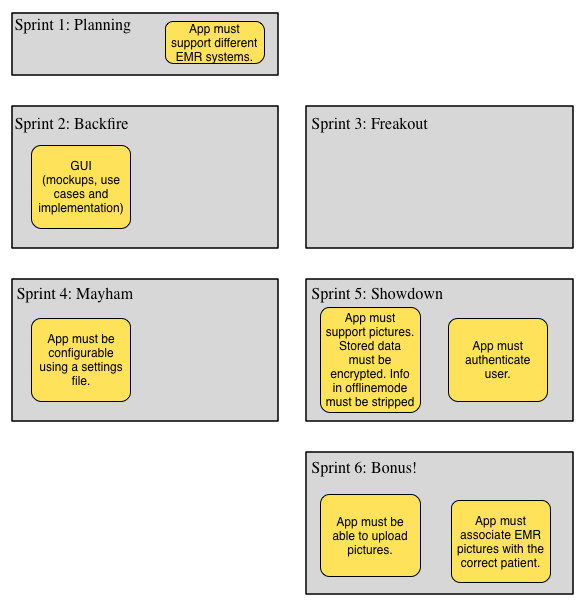
\includegraphics[scale=0.7]{img/sprint_overview_rev.png}
\caption{Revised overview of the sprints and their goals}
\label{fig:sprinter_oversikt_rev}
\end{figure}


\subsubsection{Work distribution}
The group has also discussed the situation of work distribution. During development, research, especially in regards to the hospital information systems, has mostly been done by two group members, and for a huge part of the development process only two other group members had control over the code. This was both good and bad. Because the research done in this area has not been traditional lexical research, having two people doing most of the research had it benefits. This type of research mostly consisted of email and phone calls. You tried to ask the correct questions to the correct people, and were pointed, sometimes, in several directions in their replies. By having two people doing this research, it was easier for them to follow the trail so to speak.

Thinking about the negative aspects of doing it this way we can name a few. It’s especially important for these two group members to communicate their findings to the rest of the group. And for the remaining group members to actively take an interested in how their research is going.

Having discussed the group’s problems in regards to daily scrum meetings, the group has become aware that this process of doing the research might not have been the best. Especially if one of these group members were to fall ill for a major part of the development.

As the rest of the group struggled to keep up with the research, development of the application itself was started, and the result was the same as with the research part. The two group members that started implementing became the two members that had written almost all the code written in the first sprints, making it hard for the other group members to get into and understand the code, as they were unfamiliar with the Android development platform to begin with.

With that said, the group feels that by dividing the work this way, a lot of time was saved by doing multiple tasks at once, and that the process of catching up afterwards took much less time than it would have taken to do one task at a time.

\newpage

\subsection{Product evaluation}
\label{productEval}

This section will evaluate the design choices of the Android application and explain what the group should have done different, what is missing and considerations the customer should take in regards to the future.

\subsubsection{Requirements not met}
The only requirement not met is offline mode. A discussion on this can be found in section \ref{evaloffline}.

\subsubsection{Settings}
The settings layout for the application was designed to hold data that specifies the service and authentication information. Although the application currently only supports LDAP/LDAPS, both the code and the settings layout is structured in such a way that other protocols can be implemented on a later stage. With this in mind, the customer is advised to consider whether to expand on the current code, so to support other authentication systems, or to scrape this solution, and move this functionality over to the service. The authentication architecture was researched and developed on an early stage of the development, whereas the service needed a lot more time and refinement before it was implemented. Since the service architecture change so dramatically from its first draft, it was never considered to bundle the authentication with the pre-existing tasks. If the application was to be released internationally, the consequences of the current solution would be that the application only works with hospitals information systems using with Active Directory. 


\subsubsection{User interface}
The user interface has been a priority throughout the project, as it was considered imperative to keep the flow of the application as simple and intuitive as possible. Although the group feels that the usability requirements are fulfilled, there are still some issues that should be addressed.

Throughout the application, feedback about system status should be better. This was not a priority during development process, and as a result of this, proper feedback is missing during certain actions. As of present, the "Login"-view only gives the user an unspecific error message if something went wrong during login (e.g. wrong credentials, error connection to authentication server). The "Settings"-view also lacks proper feedback, and does not notify the user if certain settings are missing or if the device is unable to connect to the server.

It is also worth noting that the interface was designed to be used in portrait mode only, and that the customer therefore should consider restricting the application to this view. It can also be considered to add support for landscape view. For instance, if the application is to be used on an Android tablet, this functionality would accommodate nicely.


\subsubsection{Offline mode}
\label{evaloffline}
Offline mode was a feature that was given a lot of thought during the initial phase of the project. Although it was not one of the primary features requested by the customer, it was still a finesse that would make the end product a lot more versatile in its usage. As mentioned in the implementation chapter, an early version of the application supported offline mode, but as the application development progressed this feature became more and more outdated. The final version of the application is therefore released without a fully functional offline mode. With that said, there is just minor changes needed to the application, to make offline mode work again. 

Currently, the application has no restrictions on letting the user upload images, or otherwise proceed with an examination after logging in. Should the session time out, or the device loose network connectivity, the only thing that happens is that sensitive data gets stripped from the user interface. Because offline mode required database access, and the final version of the database encryption design made logging in to the application necessary to use the database, the offline mode feature was discontinued.

As a result, a full refactoring of the offline mode functionality is recommended. Instead of stripping sensitive data during offline mode, the (already implemented) session system should be used. Although this restricts usage to users that have logged in at least once, it gives the great feature of full offline functionality. The doctor can log in as usual, and can conduct an examination. When the user arrives to the "Upload"-view, he should get the option of saving the examination, rather than uploading it.
This refactoring would require minor changes to the session system to support authenticating through checking database access when no network is available. For security reason, this would also require built-in brute-force detection.
The user should also be informed when the session has timed out or connection has been lost and get the option to log in again.

\subsubsection{Security}
Making sure the application satisfied the security requirements, was the most important aspect of this project. Before these requirements can be considered to be fulfilled, certain issues needs to be addressed. 

One of the most important issues is that the department credentials (as mentioned in section \ref{serviceDescription}) currently is stored in SharedPreferences. Although encrypted, this  solution is not considered a secure enough. Instead, these credentials should reside in each doctor’s encrypted database. Whereas the current application is designed to prompt the technical user for these credentials, the final version should prompt the doctor during first time login. 

Among other safety issues, proper deletion of images has not yet been implemented. In the current implementation, the application only receives the path of each image, and removes this path after upload. After images are uploaded, it is reasonable to assume that the images no longer serves any practical use to the user, and that they therefore should be deleted. 

Because of a bug, the application will currently not delete all data when the application is reconfigured. This should be considered as a major security threat, as a malicious service can replace the original without the users knowing.

The "Delete everything"-option in the settings menu is currently not password protected, which enable a malicious user to delete data. Although not a major security concern, this could still lead to loss of data not yet uploaded to the server. Of the bigger potential safety issues, the encryption library used with the database, SLQCipher, currently prints stack traces if the password attempted to decrypt the database with is wrong, caused when the authentication password is changed. See technical risk 1.4 in Appendix \ref{technicalrisks}.

To improve on the current security measures, the customer should also consider implementing brute force detection. Given that the offline mode functionality is refactored as described above, it would be possible to brute force user credentials while the application is offline.


\subsubsection{Service}
The service ended up being the biggest feature in the application. The interoperability that comes with the service implementation gives the application the potential to work with any hospital information system in the world. Whilst the application currently sends its messages using ArrayLists, the final product should rather depend on HashMaps. HashMaps is a lot more scalable, and are therefore easier to maintain. Using HashMaps renders the order of the data in messages irrelevant, whilst this order of the message is currently imperative if the message is to be interpreted correctly. 

In addition to refactoring the lists, the error message currently in use should also be assessed. The current error system is intended to send a Boolean value with the message, where the Boolean is dependent on the on the outcome of the operation (successful or not). If the Boolean is false, an error message is also attached. 

Since the application cannot vouch for the content of this message, the message system should be redesigned. An array of error codes should be designed, so that the service can return a known error to the application. Based on the error code, the application should display a relevant error to the user. 

In regards to the backup service developed during this project, this service should not be used during production. The license for the iText library (see section\ref{itextlib}) does not cover commercial use without purchasing the proper licence.

\subsubsection{Session}
The session feature was implemented to require that the user logged in only once during a given time interval. As described in section \ref{sessionimplement}, the session is also used to check network connectivity. To support the necessary changes to offline mode described in section \ref{evaloffline}, the validation and login methods should be changed to use the database to authenticate when no network is available.

\subsubsection{Application logic}
Some of the logic done in the application must be assessed if the application is to be released internationally. The patient's date of birth is currently based on the patient's SSN, which is not the case in many other countries (e.g. United States). The ID ascertained through the automatic scan is also assumed to be the patients SSN, which also is not the case in every other country. In many other systems this ID is an ID generated by PAS, which currently is not supported by the service system. 

A new examination should be created on start up, not in the examination view. Today, examination objects are created first when the examination activity starts, and examinations will therefore be overwritten if they do not reach this activity. 

\subsubsection{The code itself}
Time consuming or resource intensive tasks should run on their own thread. This is not yet implemented during automatic identification using the QR scanner, and should be addressed. In respect to the code we have produced, it should be reviewed in order to identify additional patterns and simplifications that would reduce the code complexity, give better performance as well as better re-use of code through polymorphic variants. Examples of code that should be reused is AlertDialogs for writing examination, and image comments as well as a dialog for logging in. How the application handles exceptions should also be reviewed. 

\subsubsection{Final release}
Before a final release, tests should be conducted, including unit testing and further security testing. As previously mentioned, the group does not consider itself qualified to test the application to the extent necessary to claim it to be safe for use.  

As of now, the application does not provide restrictions to which file types that can be sent to the service. This was intentionally left undone, as it was decided that this was a decision the customer should take. 

Since the application developed during this project was intended as a proof of concept, we were not reluctant in using open source libraries. Before a release, the customer should consider to implement their own functionality for both QR-scanning and image viewing, as well as getting a commercial license for the SQLCipher encryption library. 
A new feature the customer might also consider implementing, is functionality allowing the user to draw or annotate on to images on post examination. However, if this is to be considered, further research should be conducted in order to uncover if this is a feature the industry would benefit by having. With that said, the feedback the group has received when suggesting this feature for individuals in the industry, has been entirely positive.

Although not described during this report, the customer expressed desire to allow for the user to use voice recordings during the examination. This feature has not been worked on, but during development, Android's native speech-to-text feature has been tested while adding notes. This feature has worked exceptionally well when dictating in English, and is a technology the customer might want to look further into. 

\glsaddall
\printnoidxglossary[sort=word]

\newpage
\printbibliography[heading=bibintoc]

\newpage
\listoffigures

\newpage
\listoftables

%appendices
\begin{appendices}
\section{Usability testing}
\label{usability}

The group first worked out a design prototype, and did a couple of internal usability tests. Afterwards we felt that our design was ready to be tested on external users. Ideally our external users would be doctors or other medical personnel, especially since these are the people who will be using our app, but because of a tight time schedule, and eagerness to complete all of the issues in sprint 2, our priority felt best used in completing the usability tests as quick as possible. This so that we could start  implementing the actual GUI. That’s why we did our usability tests on computer science students, among others.

Before we started the usability test we presented the intended area of use that our app would be operating, and asked the users to imagine themselves as a doctor or a radiologist. The compound scenario for the test was that you’d just completed examining a patient with the ultrasound device know as VScan. You are left with with three pictures you want to attach to the patients medical record. To attach these pictures with the current patient in the most easy way you decide to use our app.

We then presented our test subjects with four scenarios
\begin{itemize}
    \item Scenario 1 - User logs in: To log in to the application, the user must input a username (radiologist) and a password(abc).         Use this information to log in to our application.

    \item Scenario 2 - Choose pictures: You are prompted with a list of pictures from an earlier examination of a patient. You wish         to delete picture 1, and only use picture 3. 
    
    \item Scenario 3 - Look up patient. You know the social security number\\(12345678901) of your patient, and wish to use this number to look up the patient. 
    
	\item Scenario 4 - Upload results from an examination: You have chosen the pictures you wish to upload, and have identified your patient. You now wish to upload these pictures and in addition add a note that “It’s a boy”. Upload the pictures to the patients health record. 
\end{itemize}

\subsection{Views}

\begin{figure}[H]
\centering
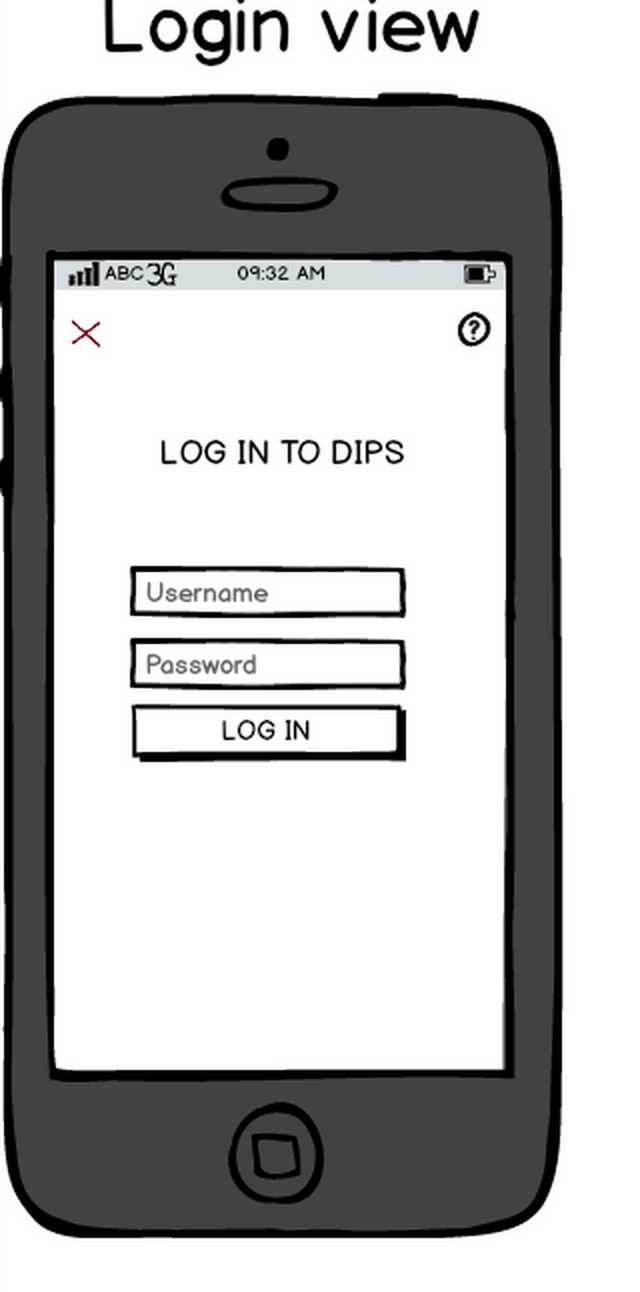
\includegraphics[scale=0.20]{img/mockups/login_view.png}
\caption{Login view}
\label{loginmock}
\end{figure}
We did not experience any issues while testing the login view (Figure \ref{loginmock}). As expected, the user clicked the username/password fields to input this information respectively. 


\begin{figure}[H]
\centering
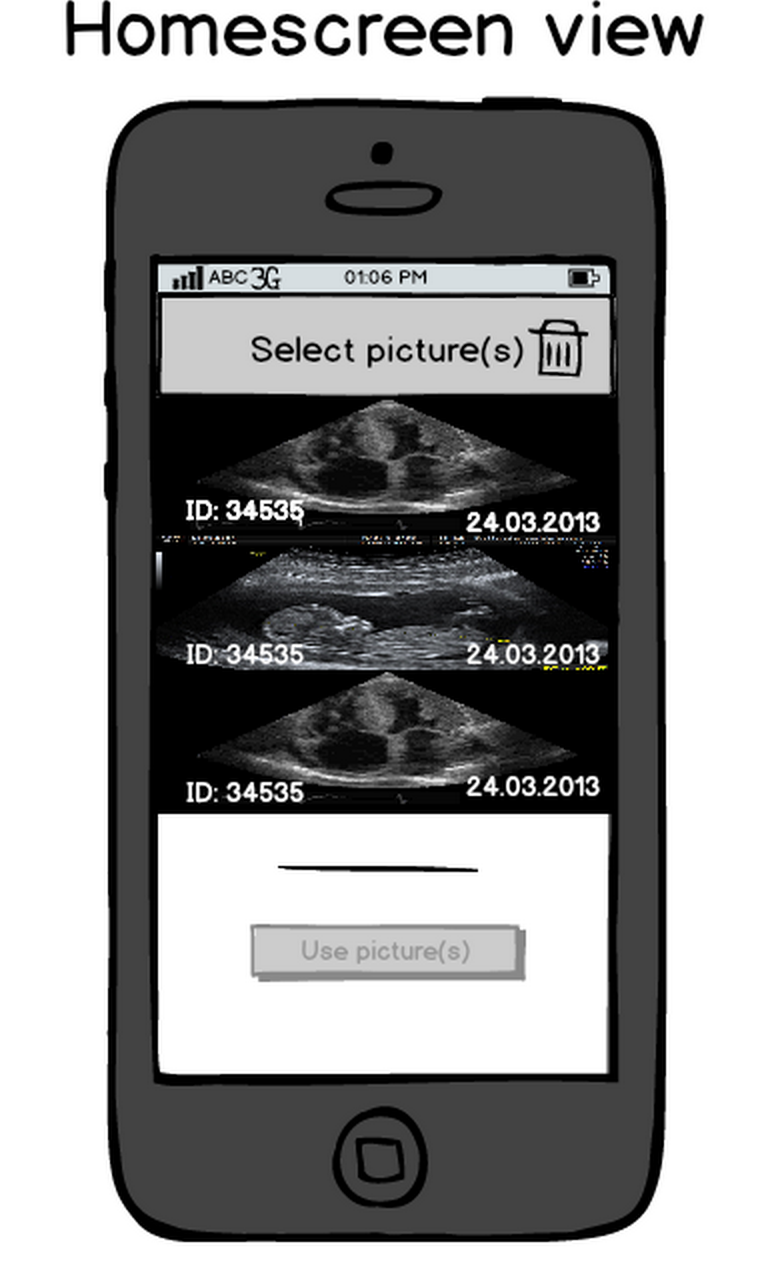
\includegraphics[scale=0.20]{img/mockups/homescreen_view.png}
\caption{Homescreen view}
\label{homemock}
\end{figure}
During testing of the home screen view (Figure \ref{homemock}), most users understood how to select the images. When they first understood how to select pictures, it seemed to be intuitive that they could delete them by selecting the delete icon, and in the same way choose which pictures to use, and proceed with the examination. 

\begin{figure}[H]
\centering
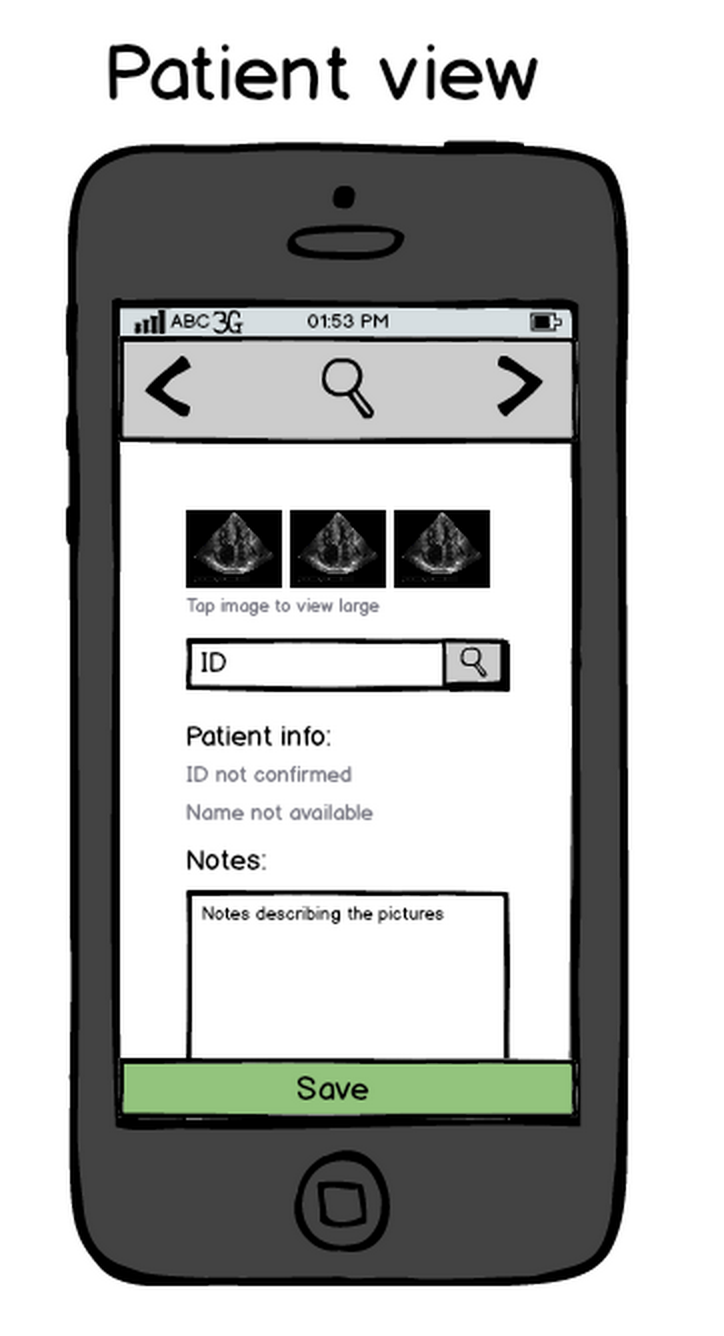
\includegraphics[scale=0.20]{img/mockups/patient_view.png}
\caption{Patient view}
\label{patientmock}
\end{figure}
We experienced several of our test subjects to be confused about the icons in the top left and right corner of the patient view (Figure \ref{patientmock}). In addition the magnifying glass icon made some subjects think that one could identify a patient by pressing it (as a button). 

\begin{figure}[H]
\centering
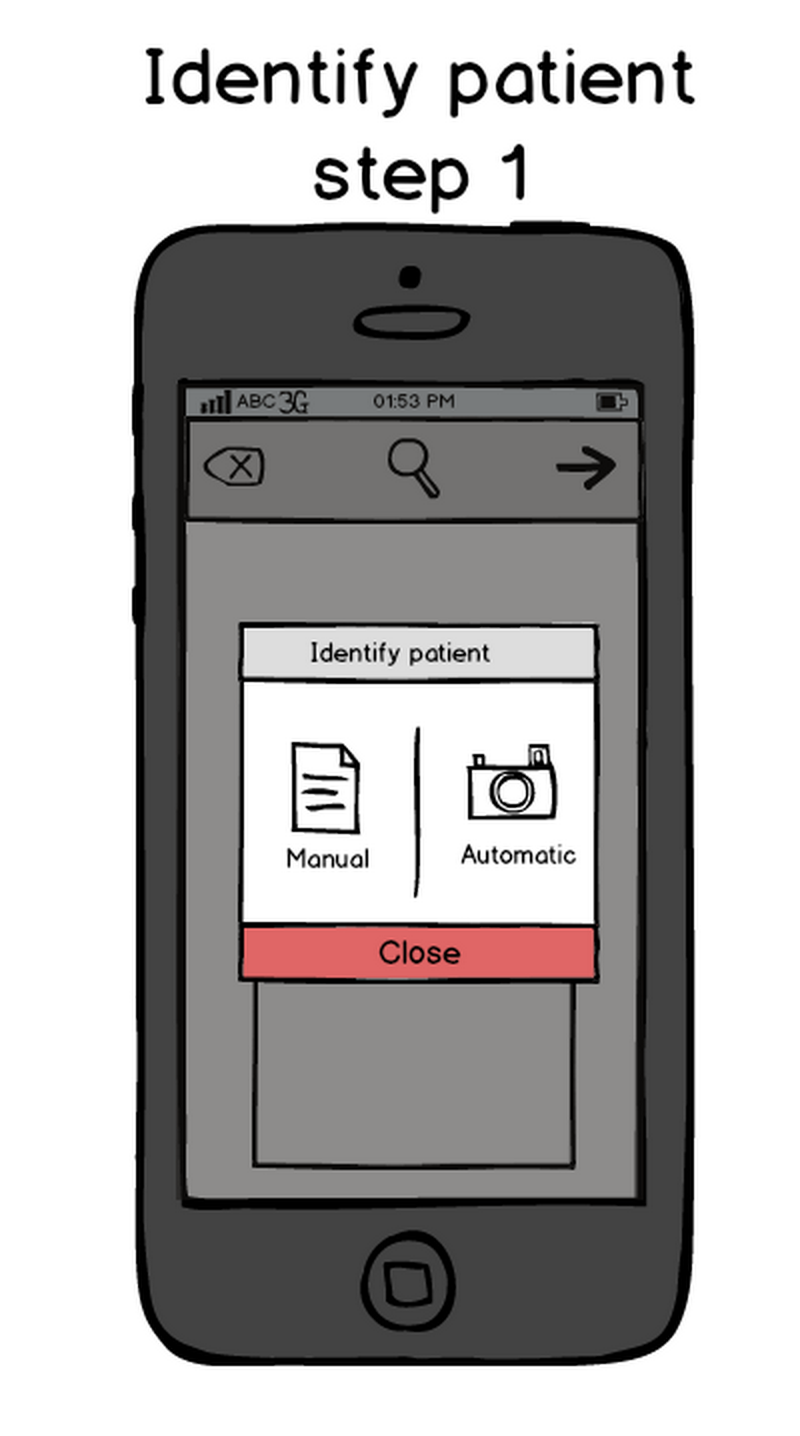
\includegraphics[scale=0.20]{img/mockups/identify_patient_1.png}
\caption{Identify patient view step 1}
\label{identifymock1}
\end{figure}
The identify patient view turned out be as intuitive as we wanted it to be. None of the test subjects appeared to have any problems using it. Nevertheless, we did (in retrospect) discover that the icons used could have been more self explaining. E.g. the automatic identification icon might have been more self explaining as a QR code icon, than a camera icon.

\begin{figure}[H]
\centering
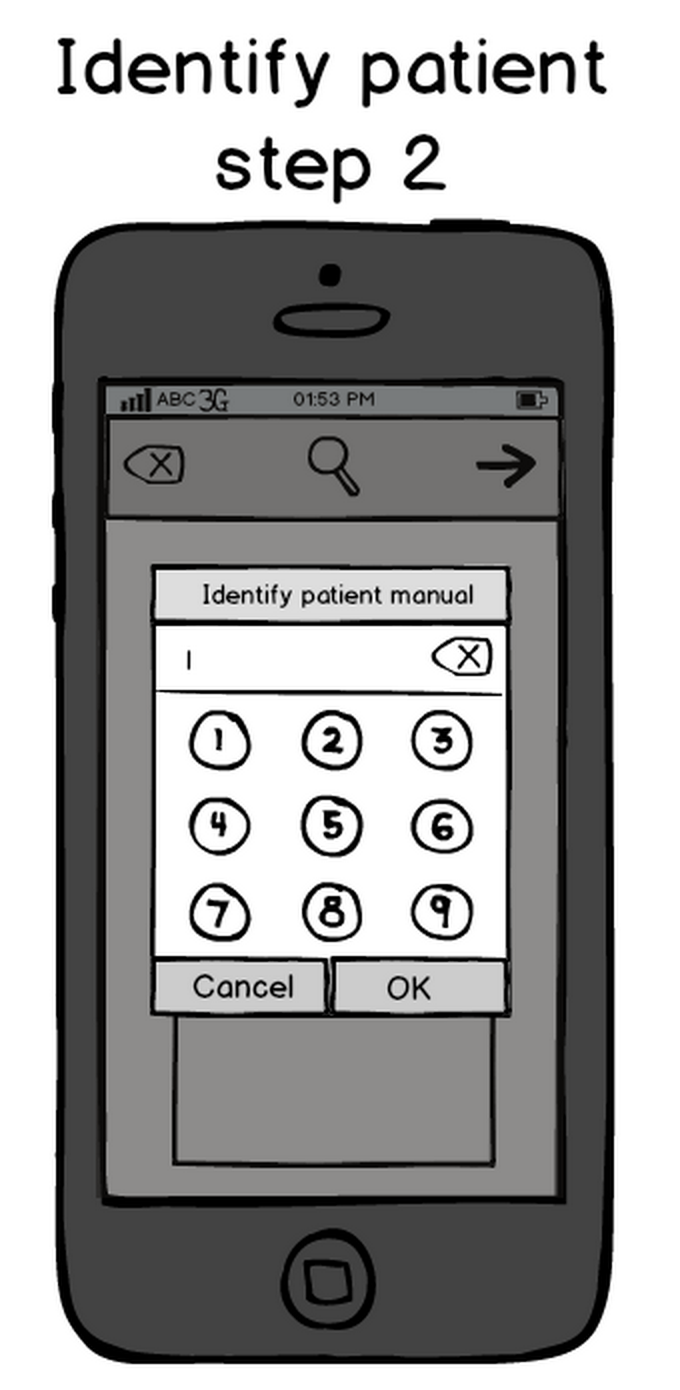
\includegraphics[scale=0.20]{img/mockups/identify_patient_2.png}
\caption{Identify patient view step 2}
\label{identifymock2}
\end{figure}
No issues were discovered while testing this view. The subjects understood that input was entered through the numerical keyboard on the screen.

\begin{figure}[H]
\centering
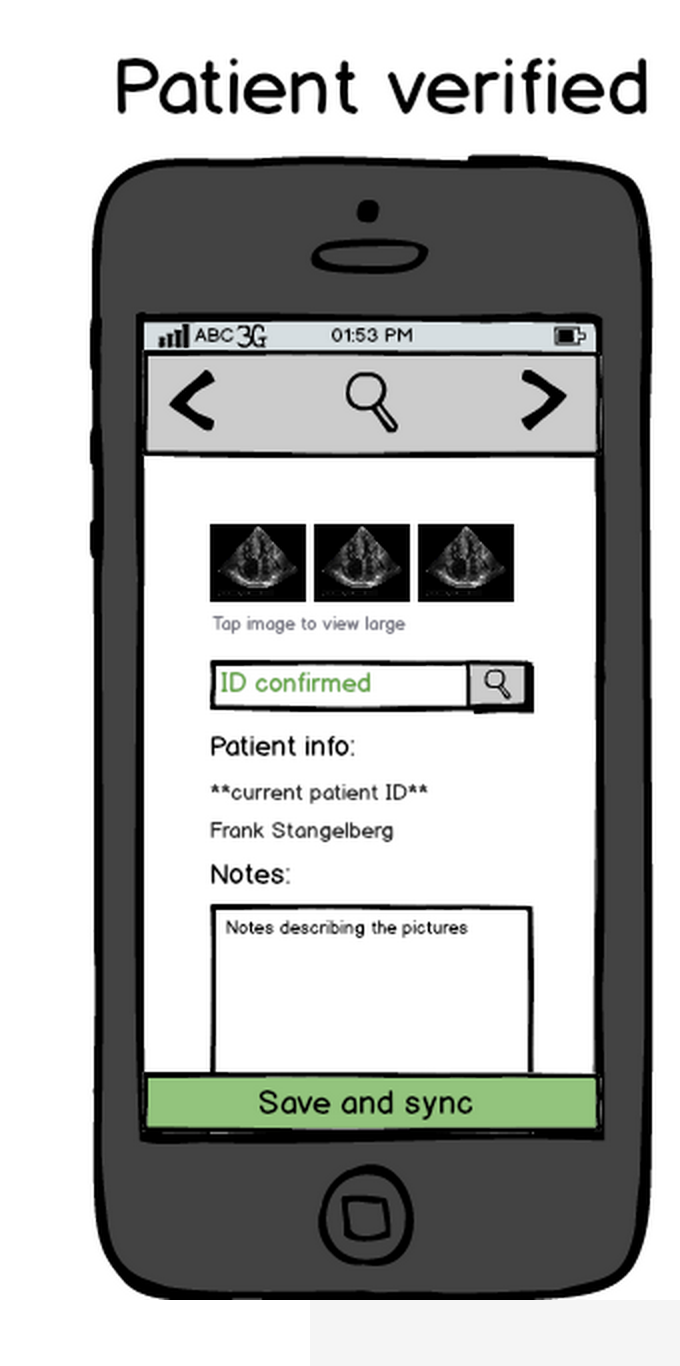
\includegraphics[scale=0.20]{img/mockups/patient_verified.png}
\caption{Patient verified view}
\label{verifymock}
\end{figure}
The patient verified view also had another problem after the patient had been identified. The “Save and sync” button at the bottom of the screen were not experienced as an actual button by the test subjects. To the contrary, this button was perceived as information.

\subsection{Conclusion}
During the usability test several potential issues were detected. Certain icons needs to be improved in order to meet the projects criteria for usability. We also established that the intended imaging functionality needs some adjustments in order to seem more intuitive and more easy to use. 

We feel that this round of usability tests have given us great feedback and insight in regards to how to proceed with our design. We were prepared to do a lot of changes in regards to how our design looked before the usability test, and as information and feedback was collected, did the respective changes which we felt was required. Our design now feels a lot more polished, but we’re prepared to do changes to make it as close to perfect as it can be.

\section{Test Case}
\label{testdoc}
This is the Test Case document which includes all component tests and the test results. As well as the list of test modules.

\subsection{Test Components}
\label{testitems}

This section lists all modules that were tested, with the related requirements.

\begin{table}[H]
\renewcommand{\arraystretch}{1.2}
\centering
\begin{tabular}{|c|c|c|c|}
\hline
Item & Description & Related Requirement\\ 
\hline
UI\textunderscore0001 & Login & 3\\ 
\hline
UI\textunderscore0002 & Identify Patient & 4\\ 
\hline
UI\textunderscore0003 & Examination View & 5,9,16,17\\ 
\hline
UI\textunderscore0004 & Image and Comments View & 15\\ 
\hline
UI\textunderscore0005 & Not yet uploaded list & 14\\ 
\hline
UI\textunderscore0006 & Review and Upload & 5,11\\ 
\hline
UI\textunderscore0007 & Settings menu & 1,15\\ 
\hline
SYS\textunderscore0001 & Take input from launcher app & 2\\
\hline
NET\textunderscore0001 & Upload to EMR & 5,8\\ 
\hline
NET\textunderscore0002 & Disconnect & 12\\ 
\hline
NET\textunderscore0003 & Download Patient Information & 4,7\\
\hline
SEC\textunderscore0001 & Security Based on Risks & SEC1, 13, 10, 18 \\
\hline
\hline
\end{tabular}
\end{table}


\subsection{Individual Tests}
\label{testcase}

The first value is the \emph{TestID} field is a reference to the \emph{Item} value in the previous section followed by an incremental value within each TestID. The \emph{dependencies} covers dependencies to other modules listed in the previous section.

\begin{table}[H] \renewcommand{\arraystretch}{1.2}
\begin{tabular}{|p{3cm}|p{9.5cm}|}

\hline

TestID & \begin{tabular}[c]{@{}l@{}}
UI\textunderscore0001.1
\end{tabular} \\ \hline

Description & \begin{tabular}[c]{@{}l@{}}
Login with correct user credentials
\end{tabular} \\ \hline

Dependencies & \begin{tabular}[c]{@{}l@{}} 
SYS\textunderscore0001
\end{tabular} \\ \hline

Precondition & \begin{tabular}[c]{@{}l@{}}
The app has started with network connectivity
\end{tabular} \\ \hline

Input & \begin{tabular}[c]{@{}l@{}}
Correct username and password
\end{tabular} \\ \hline

Expected output & \begin{tabular}[c]{@{}l@{}}
The user get logged in
\end{tabular} \\ \hline

Postcondition & \begin{tabular}[c]{@{}l@{}}
The app presents the next view, depending on\\ the launch variables
\end{tabular} \\ \hline

Result & \begin{tabular}[c]{@{}l@{}} 
Pass
\end{tabular} \\ \hline

\end{tabular}
\end{table}


\begin{table}[H] \renewcommand{\arraystretch}{1.2}
\begin{tabular}{|p{3cm}|p{9.5cm}|}

\hline

TestID & \begin{tabular}[c]{@{}l@{}}
UI\textunderscore0001.2
\end{tabular} \\ \hline

Description & \begin{tabular}[c]{@{}l@{}}
Login with wrong password and correct username
\end{tabular} \\ \hline

Dependencies & \begin{tabular}[c]{@{}l@{}}
SYS\textunderscore0001
\end{tabular} \\ \hline

Precondition & \begin{tabular}[c]{@{}l@{}}
The app has started with network connectivity
\end{tabular} \\ \hline

Input & \begin{tabular}[c]{@{}l@{}}
Correct username, wrong password
\end{tabular} \\ \hline

Expected output & \begin{tabular}[c]{@{}l@{}}
Error message: "Wrong username and/or password"
\end{tabular} \\ \hline

Postcondition & \begin{tabular}[c]{@{}l@{}}
The password field is cleared
\end{tabular} \\ \hline

Result & \begin{tabular}[c]{@{}l@{}} 
Pass
\end{tabular} \\ \hline

\end{tabular}
\end{table}


\begin{table}[H] \renewcommand{\arraystretch}{1.2}

\begin{tabular}{|p{3cm}|p{9.5cm}|}
\hline

TestID & \begin{tabular}[c]{@{}l@{}}
UI\textunderscore0001.3
\end{tabular} \\ \hline

Description & \begin{tabular}[c]{@{}l@{}}
Login with wrong username
\end{tabular} \\ \hline

Dependencies & \begin{tabular}[c]{@{}l@{}}
SYS\textunderscore0001
\end{tabular} \\ \hline

Precondition & \begin{tabular}[c]{@{}l@{}}
The app has started with network connectivity
\end{tabular} \\ \hline

Input & \begin{tabular}[c]{@{}l@{}}
Wrong username
\end{tabular} \\ \hline

Expected output & \begin{tabular}[c]{@{}l@{}}
Error message: "Wrong username and/or password"
\end{tabular} \\ \hline

Postcondition & \begin{tabular}[c]{@{}l@{}}
The password field is cleared
\end{tabular} \\ \hline

Result & \begin{tabular}[c]{@{}l@{}} 
Pass
\end{tabular} \\ \hline

\end{tabular}
\end{table}


\begin{table}[H] \renewcommand{\arraystretch}{1.2}

\begin{tabular}{|p{3cm}|p{9.5cm}|}
\hline

TestID & \begin{tabular}[c]{@{}l@{}}
UI\textunderscore0001.4
\end{tabular} \\ \hline

Description & \begin{tabular}[c]{@{}l@{}}
Login with a password but no username
\end{tabular} \\ \hline

Dependencies & \begin{tabular}[c]{@{}l@{}}
SYS\textunderscore0001
\end{tabular} \\ \hline

Precondition & \begin{tabular}[c]{@{}l@{}}
The app has started with connection
\end{tabular} \\ \hline

Input & \begin{tabular}[c]{@{}l@{}}
No username, a password	
\end{tabular} \\ \hline

Expected output & \begin{tabular}[c]{@{}l@{}}
Error message: "Wrong username and/or password"
\end{tabular} \\ \hline

Postcondition & \begin{tabular}[c]{@{}l@{}}
The password field is cleared
\end{tabular} \\ \hline

Result & \begin{tabular}[c]{@{}l@{}} 
Pass
\end{tabular} \\ \hline

\end{tabular}
\end{table}


\begin{table}[H] \renewcommand{\arraystretch}{1.2}

\begin{tabular}{|p{3cm}|p{9.5cm}|}
\hline

TestID & \begin{tabular}[c]{@{}l@{}}
UI\textunderscore0001.5
\end{tabular} \\ \hline

Description & \begin{tabular}[c]{@{}l@{}}
Login with a username but no password
\end{tabular} \\ \hline

Dependencies & \begin{tabular}[c]{@{}l@{}}
SYS\textunderscore0001
\end{tabular} \\ \hline

Precondition & \begin{tabular}[c]{@{}l@{}}
The app has started with network connectivity
\end{tabular} \\ \hline

Input & \begin{tabular}[c]{@{}l@{}}
Correct username, no password
\end{tabular} \\ \hline

Expected output & \begin{tabular}[c]{@{}l@{}}
Error message: "Wrong username and/or password"
\end{tabular} \\ \hline

Postcondition & \begin{tabular}[c]{@{}l@{}}
The password field is cleared
\end{tabular} \\ \hline

Result & \begin{tabular}[c]{@{}l@{}} 
Pass
\end{tabular} \\ \hline

\end{tabular}
\end{table}


\begin{table}[H] \renewcommand{\arraystretch}{1.2}

\begin{tabular}{|p{3cm}|p{9.5cm}|}
\hline

TestID & \begin{tabular}[c]{@{}l@{}}
UI\textunderscore0001.6
\end{tabular} \\ \hline

Description & \begin{tabular}[c]{@{}l@{}}
Login with no password nor username
\end{tabular} \\ \hline

Dependencies & \begin{tabular}[c]{@{}l@{}}
SYS\textunderscore0001
\end{tabular} \\ \hline

Precondition & \begin{tabular}[c]{@{}l@{}}
The app has started with connection
\end{tabular} \\ \hline

Input & \begin{tabular}[c]{@{}l@{}}
No input
\end{tabular} \\ \hline

Expected output & \begin{tabular}[c]{@{}l@{}}
Error message: "Wrong username and/or password"
\end{tabular} \\ \hline

Postcondition & \begin{tabular}[c]{@{}l@{}}
The password field is cleared
\end{tabular} \\ \hline

Result & \begin{tabular}[c]{@{}l@{}} 
Pass
\end{tabular} \\ \hline

\end{tabular}
\end{table}


\begin{table}[H] \renewcommand{\arraystretch}{1.2}

\begin{tabular}{|p{3cm}|p{9.5cm}|}
\hline

TestID & \begin{tabular}[c]{@{}l@{}}
UI\textunderscore0001.7
\end{tabular} \\ \hline

Description & \begin{tabular}[c]{@{}l@{}}
Cancel operation
\end{tabular} \\ \hline

Dependencies & \begin{tabular}[c]{@{}l@{}}
SYS\textunderscore0001
\end{tabular} \\ \hline

Precondition & \begin{tabular}[c]{@{}l@{}}
The app has started with connection
\end{tabular} \\ \hline

Input & \begin{tabular}[c]{@{}l@{}}
Cancel with the back/exit button
\end{tabular} \\ \hline

Expected output & \begin{tabular}[c]{@{}l@{}}
The app closes
\end{tabular} \\ \hline

Postcondition & \begin{tabular}[c]{@{}l@{}}
The app is closed
\end{tabular} \\ \hline

Result & \begin{tabular}[c]{@{}l@{}} 
Pass
\end{tabular} \\ \hline

\end{tabular}
\end{table}


\begin{table}[H] \renewcommand{\arraystretch}{1.2}

\begin{tabular}{|p{3cm}|p{9.5cm}|}
\hline

TestID & \begin{tabular}[c]{@{}l@{}}
UI\textunderscore0001.8
\end{tabular} \\ \hline

Description & \begin{tabular}[c]{@{}l@{}}
Go to the settings view
\end{tabular} \\ \hline

Dependencies & \begin{tabular}[c]{@{}l@{}}
SYS\textunderscore0001
\end{tabular} \\ \hline

Precondition & \begin{tabular}[c]{@{}l@{}}
The app has started
\end{tabular} \\ \hline

Input & \begin{tabular}[c]{@{}l@{}}
Press the settings icon
\end{tabular} \\ \hline

Expected output & \begin{tabular}[c]{@{}l@{}}
View changes
\end{tabular} \\ \hline

Postcondition & \begin{tabular}[c]{@{}l@{}}
Settings view is shown
\end{tabular} \\ \hline

Result & \begin{tabular}[c]{@{}l@{}} 
Pass
\end{tabular} \\ \hline

\end{tabular}
\end{table}


\begin{table}[H] \renewcommand{\arraystretch}{1.2}

\begin{tabular}{|p{3cm}|p{9.5cm}|}
\hline

TestID & \begin{tabular}[c]{@{}l@{}}
UI\textunderscore0002.1
\end{tabular} \\ \hline

Description & \begin{tabular}[c]{@{}l@{}}
Enter an existing SSN 
\end{tabular} \\ \hline

Dependencies & \begin{tabular}[c]{@{}l@{}}
UI\textunderscore0001
\end{tabular} \\ \hline

Precondition & \begin{tabular}[c]{@{}l@{}}
The user has logged in
\end{tabular} \\ \hline

Input & \begin{tabular}[c]{@{}l@{}}
Valid SSN 
\end{tabular} \\ \hline

Expected output & \begin{tabular}[c]{@{}l@{}}
The app downloads the patient information
\end{tabular} \\ \hline

Postcondition & \begin{tabular}[c]{@{}l@{}}
The app presents the examination view
\end{tabular} \\ \hline

Result & \begin{tabular}[c]{@{}l@{}} 
Pass
\end{tabular} \\ \hline

\end{tabular}
\end{table}


\begin{table}[H] \renewcommand{\arraystretch}{1.2}

\begin{tabular}{|p{3cm}|p{9.5cm}|}
\hline

TestID & \begin{tabular}[c]{@{}l@{}}
UI\textunderscore0002.2
\end{tabular} \\ \hline

Description & \begin{tabular}[c]{@{}l@{}}
No input
\end{tabular} \\ \hline

Dependencies & \begin{tabular}[c]{@{}l@{}}
UI\textunderscore0001
\end{tabular} \\ \hline

Precondition & \begin{tabular}[c]{@{}l@{}}
The user has logged in
\end{tabular} \\ \hline

Input & \begin{tabular}[c]{@{}l@{}}
No input
\end{tabular} \\ \hline

Expected output & \begin{tabular}[c]{@{}l@{}}
Error message: "Invalid SSN"
\end{tabular} \\ \hline

Postcondition & \begin{tabular}[c]{@{}l@{}}
Ssn field is cleared
\end{tabular} \\ \hline

Result & \begin{tabular}[c]{@{}l@{}} 
Pass
\end{tabular} \\ \hline

\end{tabular}
\end{table}


\begin{table}[H] \renewcommand{\arraystretch}{1.2}

\begin{tabular}{|p{3cm}|p{9.5cm}|}
\hline

TestID & \begin{tabular}[c]{@{}l@{}}
UI\textunderscore0002.3
\end{tabular} \\ \hline

Description & \begin{tabular}[c]{@{}l@{}}
Enter invalid SSN
\end{tabular} \\ \hline

Dependencies & \begin{tabular}[c]{@{}l@{}}
UI\textunderscore0001
\end{tabular} \\ \hline

Precondition & \begin{tabular}[c]{@{}l@{}}
The user has logged in
\end{tabular} \\ \hline

Input & \begin{tabular}[c]{@{}l@{}}
Invalid SSN
\end{tabular} \\ \hline

Expected output & \begin{tabular}[c]{@{}l@{}}
Error message: "Invalid SSN"
\end{tabular} \\ \hline

Postcondition & \begin{tabular}[c]{@{}l@{}}
Ssn field is cleared
\end{tabular} \\ \hline

Result & \begin{tabular}[c]{@{}l@{}} 
Pass
\end{tabular} \\ \hline

\end{tabular}
\end{table}


\begin{table}[H] \renewcommand{\arraystretch}{1.2}

\begin{tabular}{|p{3cm}|p{9.5cm}|}
\hline

TestID & \begin{tabular}[c]{@{}l@{}}
UI\textunderscore0002.4
\end{tabular} \\ \hline

Description & \begin{tabular}[c]{@{}l@{}}
Cancel operation
\end{tabular} \\ \hline

Dependencies & \begin{tabular}[c]{@{}l@{}}
UI\textunderscore0001
\end{tabular} \\ \hline

Precondition & \begin{tabular}[c]{@{}l@{}}
The user has logged in
\end{tabular} \\ \hline

Input & \begin{tabular}[c]{@{}l@{}}
Cancel with the back/exit button
\end{tabular} \\ \hline

Expected output & \begin{tabular}[c]{@{}l@{}}
The app closes or returns to the examination.
\end{tabular} \\ \hline

Postcondition & \begin{tabular}[c]{@{}l@{}}
The app is closed or the examination is shown.
\end{tabular} \\ \hline

Result & \begin{tabular}[c]{@{}l@{}} 
Pass
\end{tabular} \\ \hline

\end{tabular}
\end{table}


\begin{table}[H] \renewcommand{\arraystretch}{1.2}

\begin{tabular}{|p{3cm}|p{9.5cm}|}
\hline

TestID & \begin{tabular}[c]{@{}l@{}}
UI\textunderscore0003.1
\end{tabular} \\ \hline

Description & \begin{tabular}[c]{@{}l@{}}
Press "Add comments to images"
\end{tabular} \\ \hline

Dependencies & \begin{tabular}[c]{@{}l@{}}
UI\textunderscore0002 or UI\textunderscore0005
\end{tabular} \\ \hline

Precondition & \begin{tabular}[c]{@{}l@{}}
The user has opened an examination
\end{tabular} \\ \hline

Input & \begin{tabular}[c]{@{}l@{}}
Press "Add comments to images" button
\end{tabular} \\ \hline

Expected output & \begin{tabular}[c]{@{}l@{}}
Button is clickable and changes view
\end{tabular} \\ \hline

Postcondition & \begin{tabular}[c]{@{}l@{}}
The images and comments view is presented
\end{tabular} \\ \hline

Result & \begin{tabular}[c]{@{}l@{}} 
Pass
\end{tabular} \\ \hline

\end{tabular}
\end{table}


\begin{table}[H] \renewcommand{\arraystretch}{1.2}

\begin{tabular}{|p{3cm}|p{9.5cm}|}
\hline

TestID & \begin{tabular}[c]{@{}l@{}}
UI\textunderscore0003.2
\end{tabular} \\ \hline

Description & \begin{tabular}[c]{@{}l@{}}
Press "Review and upload"
\end{tabular} \\ \hline

Dependencies & \begin{tabular}[c]{@{}l@{}}
UI\textunderscore0002 or UI\textunderscore0005
\end{tabular} \\ \hline

Precondition & \begin{tabular}[c]{@{}l@{}}
The user has opened an examination
\end{tabular} \\ \hline

Input & \begin{tabular}[c]{@{}l@{}}
Press "Review and upload" button
\end{tabular} \\ \hline

Expected output & \begin{tabular}[c]{@{}l@{}}
Button is clickable and changes view
\end{tabular} \\ \hline

Postcondition & \begin{tabular}[c]{@{}l@{}}
The review and upload view is presented
\end{tabular} \\ \hline

Result & \begin{tabular}[c]{@{}l@{}} 
Pass
\end{tabular} \\ \hline

\end{tabular}
\end{table}


\begin{table}[H] \renewcommand{\arraystretch}{1.2}

\begin{tabular}{|p{3cm}|p{9.5cm}|}
\hline

TestID & \begin{tabular}[c]{@{}l@{}}
UI\textunderscore0003.3
\end{tabular} \\ \hline

Description & \begin{tabular}[c]{@{}l@{}}
Cancel operation
\end{tabular} \\ \hline

Dependencies & \begin{tabular}[c]{@{}l@{}}
UI\textunderscore0002 or UI\textunderscore0005
\end{tabular} \\ \hline

Precondition & \begin{tabular}[c]{@{}l@{}}
The user has opened an examination
\end{tabular} \\ \hline

Input & \begin{tabular}[c]{@{}l@{}}
Cancel with the back/exit button
\end{tabular} \\ \hline

Expected output & \begin{tabular}[c]{@{}l@{}}
The user will be prompted to save or \\discard changes
\end{tabular} \\ \hline

Postcondition & \begin{tabular}[c]{@{}l@{}}
The user can choose to save or discard the changes
\end{tabular} \\ \hline

Result & \begin{tabular}[c]{@{}l@{}} 
No prompt is shown, the app saves, and returns \\ to the list of not yet uploaded examinations
\end{tabular} \\ \hline

\end{tabular}
\end{table}


\begin{table}[H] \renewcommand{\arraystretch}{1.2}

\begin{tabular}{|p{3cm}|p{9.5cm}|}
\hline

TestID & \begin{tabular}[c]{@{}l@{}}
UI\textunderscore0003.4
\end{tabular} \\ \hline

Description & \begin{tabular}[c]{@{}l@{}}
Press "Add comment to examination"
\end{tabular} \\ \hline

Dependencies & \begin{tabular}[c]{@{}l@{}}
UI\textunderscore0002 or UI\textunderscore0005
\end{tabular} \\ \hline

Precondition & \begin{tabular}[c]{@{}l@{}}
The user has opened an examination
\end{tabular} \\ \hline

Input & \begin{tabular}[c]{@{}l@{}}
Press "Add comment to examination" button
\end{tabular} \\ \hline

Expected output & \begin{tabular}[c]{@{}l@{}}
Button is clickable and changes view
\end{tabular} \\ \hline

Postcondition & \begin{tabular}[c]{@{}l@{}}
The user is presented with a view to enter text
\end{tabular} \\ \hline

Result & \begin{tabular}[c]{@{}l@{}} 
Pass
\end{tabular} \\ \hline

\end{tabular}
\end{table}


\begin{table}[H] \renewcommand{\arraystretch}{1.2}

\begin{tabular}{|p{3cm}|p{9.5cm}|}
\hline

TestID & \begin{tabular}[c]{@{}l@{}}
UI\textunderscore0004.1
\end{tabular} \\ \hline

Description & \begin{tabular}[c]{@{}l@{}}
Delete Image
\end{tabular} \\ \hline

Dependencies & \begin{tabular}[c]{@{}l@{}}
UI\textunderscore0003
\end{tabular} \\ \hline

Precondition & \begin{tabular}[c]{@{}l@{}}
The user has pressed "Add comments to images"
\end{tabular} \\ \hline

Input & \begin{tabular}[c]{@{}l@{}}
Press the trashcan
\end{tabular} \\ \hline

Expected output & \begin{tabular}[c]{@{}l@{}}
Button is clickable and removes the image
\end{tabular} \\ \hline

Postcondition & \begin{tabular}[c]{@{}l@{}}
The view is updated and the previous \\image is shown
\end{tabular} \\ \hline

Result & \begin{tabular}[c]{@{}l@{}} 
Pass
\end{tabular} \\ \hline

\end{tabular}
\end{table}


\begin{table}[H] \renewcommand{\arraystretch}{1.2}

\begin{tabular}{|p{3cm}|p{9.5cm}|}
\hline

TestID & \begin{tabular}[c]{@{}l@{}}
UI\textunderscore0004.2
\end{tabular} \\ \hline

Description & \begin{tabular}[c]{@{}l@{}}
Delete Last Image
\end{tabular} \\ \hline

Dependencies & \begin{tabular}[c]{@{}l@{}}
UI\textunderscore0003
\end{tabular} \\ \hline

Precondition & \begin{tabular}[c]{@{}l@{}}
The user has pressed "Add comments to images"
\end{tabular} \\ \hline

Input & \begin{tabular}[c]{@{}l@{}}
Press the trashcan
\end{tabular} \\ \hline

Expected output & \begin{tabular}[c]{@{}l@{}}
Button is clickable, error message is shown.
\end{tabular} \\ \hline

Postcondition & \begin{tabular}[c]{@{}l@{}}
Nothing happens
\end{tabular} \\ \hline

Result & \begin{tabular}[c]{@{}l@{}} 
Pass
\end{tabular} \\ \hline

\end{tabular}
\end{table}


\begin{table}[H] \renewcommand{\arraystretch}{1.2}

\begin{tabular}{|p{3cm}|p{9.5cm}|}
\hline

TestID & \begin{tabular}[c]{@{}l@{}}
UI\textunderscore0004.3
\end{tabular} \\ \hline

Description & \begin{tabular}[c]{@{}l@{}}
Write a comment
\end{tabular} \\ \hline

Dependencies & \begin{tabular}[c]{@{}l@{}}
UI\textunderscore0003
\end{tabular} \\ \hline

Precondition & \begin{tabular}[c]{@{}l@{}}
The user has pressed "Add comments to images"
\end{tabular} \\ \hline

Input & \begin{tabular}[c]{@{}l@{}}
Press the comment button
\end{tabular} \\ \hline

Expected output & \begin{tabular}[c]{@{}l@{}}
The text input box is shown and usable
\end{tabular} \\ \hline

Postcondition & \begin{tabular}[c]{@{}l@{}}
Comment is saved, and image is shown
\end{tabular} \\ \hline

Result & \begin{tabular}[c]{@{}l@{}} 
Pass
\end{tabular} \\ \hline

\end{tabular}
\end{table}


\begin{table}[H] \renewcommand{\arraystretch}{1.2}

\begin{tabular}{|p{3cm}|p{9.5cm}|}
\hline

TestID & \begin{tabular}[c]{@{}l@{}}
UI\textunderscore0004.4
\end{tabular} \\ \hline

Description & \begin{tabular}[c]{@{}l@{}}
Swipe to the next image
\end{tabular} \\ \hline

Dependencies & \begin{tabular}[c]{@{}l@{}}
UI\textunderscore0003
\end{tabular} \\ \hline

Precondition & \begin{tabular}[c]{@{}l@{}}
The user has pressed "Add comments to images"
\end{tabular} \\ \hline

Input & \begin{tabular}[c]{@{}l@{}}
Swipe left
\end{tabular} \\ \hline

Expected output & \begin{tabular}[c]{@{}l@{}}
View is updated with next image
\end{tabular} \\ \hline

Postcondition & \begin{tabular}[c]{@{}l@{}}
Same view with new image
\end{tabular} \\ \hline

Result & \begin{tabular}[c]{@{}l@{}}
Pass
\end{tabular} \\ \hline

\end{tabular}
\end{table}


\begin{table}[H] \renewcommand{\arraystretch}{1.2}

\begin{tabular}{|p{3cm}|p{9.5cm}|}
\hline

TestID & \begin{tabular}[c]{@{}l@{}}
UI\textunderscore0004.5
\end{tabular} \\ \hline

Description & \begin{tabular}[c]{@{}l@{}}
Swipe left on last picture
\end{tabular} \\ \hline

Dependencies & \begin{tabular}[c]{@{}l@{}}
UI\textunderscore0003
\end{tabular} \\ \hline

Precondition & \begin{tabular}[c]{@{}l@{}}
The user has pressed "Add comments to images"
\end{tabular} \\ \hline

Input & \begin{tabular}[c]{@{}l@{}}
Swipe left
\end{tabular} \\ \hline

Expected output & \begin{tabular}[c]{@{}l@{}}
Nothing happens
\end{tabular} \\ \hline

Postcondition & \begin{tabular}[c]{@{}l@{}}
Same view
\end{tabular} \\ \hline

Result & \begin{tabular}[c]{@{}l@{}} 
Pass
\end{tabular} \\ \hline

\end{tabular}
\end{table}


\begin{table}[H] \renewcommand{\arraystretch}{1.2}

\begin{tabular}{|p{3cm}|p{9.5cm}|}
\hline

TestID & \begin{tabular}[c]{@{}l@{}}
UI\textunderscore0004.6
\end{tabular} \\ \hline

Description & \begin{tabular}[c]{@{}l@{}}
Swipe right on first image
\end{tabular} \\ \hline

Dependencies & \begin{tabular}[c]{@{}l@{}}
UI\textunderscore0003
\end{tabular} \\ \hline

Precondition & \begin{tabular}[c]{@{}l@{}}
The user has pressed "Add comments to images"
\end{tabular} \\ \hline

Input & \begin{tabular}[c]{@{}l@{}}
Swipe right
\end{tabular} \\ \hline

Expected output & \begin{tabular}[c]{@{}l@{}}
Nothing happens
\end{tabular} \\ \hline

Postcondition & \begin{tabular}[c]{@{}l@{}}
Same view
\end{tabular} \\ \hline

Result & \begin{tabular}[c]{@{}l@{}} 
Pass
\end{tabular} \\ \hline

\end{tabular}
\end{table}


\begin{table}[H] \renewcommand{\arraystretch}{1.2}

\begin{tabular}{|p{3cm}|p{9.5cm}|}
\hline

TestID & \begin{tabular}[c]{@{}l@{}}
UI\textunderscore0004.7
\end{tabular} \\ \hline

Description & \begin{tabular}[c]{@{}l@{}}
Cancel operation
\end{tabular} \\ \hline

Dependencies & \begin{tabular}[c]{@{}l@{}}
UI\textunderscore0003
\end{tabular} \\ \hline

Precondition & \begin{tabular}[c]{@{}l@{}}
The user has pressed "Add comments to images"
\end{tabular} \\ \hline

Input & \begin{tabular}[c]{@{}l@{}}
Cancel with the back/close button
\end{tabular} \\ \hline

Expected output & \begin{tabular}[c]{@{}l@{}}
Changes view
\end{tabular} \\ \hline

Postcondition & \begin{tabular}[c]{@{}l@{}}
The examination view is presented
\end{tabular} \\ \hline

Result & \begin{tabular}[c]{@{}l@{}} 
No changes saved
\end{tabular} \\ \hline

\end{tabular}
\end{table}


\begin{table}[H] \renewcommand{\arraystretch}{1.2}

\begin{tabular}{|p{3cm}|p{9.5cm}|}
\hline

TestID & \begin{tabular}[c]{@{}l@{}}
UI\textunderscore0005.1
\end{tabular} \\ \hline

Description & \begin{tabular}[c]{@{}l@{}}
Open an examination
\end{tabular} \\ \hline

Dependencies & \begin{tabular}[c]{@{}l@{}}
SYS\textunderscore0001
\end{tabular} \\ \hline

Precondition & \begin{tabular}[c]{@{}l@{}}
The app is started with no images
\end{tabular} \\ \hline

Input & \begin{tabular}[c]{@{}l@{}}
Press an examination, and choose edit
\end{tabular} \\ \hline

Expected output & \begin{tabular}[c]{@{}l@{}}
Opens the correct examination
\end{tabular} \\ \hline

Postcondition & \begin{tabular}[c]{@{}l@{}}
The examination view is presented
\end{tabular} \\ \hline

Result & \begin{tabular}[c]{@{}l@{}} 
Pass
\end{tabular} \\ \hline

\end{tabular}
\end{table}


\begin{table}[H] \renewcommand{\arraystretch}{1.2}

\begin{tabular}{|p{3cm}|p{9.5cm}|}
\hline

TestID & \begin{tabular}[c]{@{}l@{}}
UI\textunderscore0005.2
\end{tabular} \\ \hline

Description & \begin{tabular}[c]{@{}l@{}}
Cancel operation
\end{tabular} \\ \hline

Dependencies & \begin{tabular}[c]{@{}l@{}}
SYS\textunderscore0001
\end{tabular} \\ \hline

Precondition & \begin{tabular}[c]{@{}l@{}}
The app is started with no images
\end{tabular} \\ \hline

Input & \begin{tabular}[c]{@{}l@{}}
Cancel with the back/exit button
\end{tabular} \\ \hline

Expected output & \begin{tabular}[c]{@{}l@{}}
App closes
\end{tabular} \\ \hline

Postcondition & \begin{tabular}[c]{@{}l@{}}
The app is closed
\end{tabular} \\ \hline

Result & \begin{tabular}[c]{@{}l@{}} 
Pass
\end{tabular} \\ \hline

\end{tabular}
\end{table}


\begin{table}[H] \renewcommand{\arraystretch}{1.2}

\begin{tabular}{|p{3cm}|p{9.5cm}|}
\hline

TestID & \begin{tabular}[c]{@{}l@{}}
UI\textunderscore0005.3
\end{tabular} \\ \hline

Description & \begin{tabular}[c]{@{}l@{}}
Delete examination
\end{tabular} \\ \hline

Dependencies & \begin{tabular}[c]{@{}l@{}}
SYS\textunderscore0001
\end{tabular} \\ \hline

Precondition & \begin{tabular}[c]{@{}l@{}}
The app is started with no images
\end{tabular} \\ \hline

Input & \begin{tabular}[c]{@{}l@{}}
Click one of the examinations and press the \\delete button, then confirm the deletion
\end{tabular} \\ \hline

Expected output & \begin{tabular}[c]{@{}l@{}}
The user is presented with a confirmation dialog, \\ then returns to the examination list
\end{tabular} \\ \hline

Postcondition & \begin{tabular}[c]{@{}l@{}}
The examination list is presented without \\the deleted examination
\end{tabular} \\ \hline

Result & \begin{tabular}[c]{@{}l@{}} 
Pass
\end{tabular} \\ \hline

\end{tabular}
\end{table}


\begin{table}[H] \renewcommand{\arraystretch}{1.2}

\begin{tabular}{|p{3cm}|p{9.5cm}|}
\hline

TestID & \begin{tabular}[c]{@{}l@{}}
UI\textunderscore0005.4
\end{tabular} \\ \hline

Description & \begin{tabular}[c]{@{}l@{}}
Log out
\end{tabular} \\ \hline

Dependencies & \begin{tabular}[c]{@{}l@{}}
SYS\textunderscore0001
\end{tabular} \\ \hline

Precondition & \begin{tabular}[c]{@{}l@{}}
The app is started with no images
\end{tabular} \\ \hline

Input & \begin{tabular}[c]{@{}l@{}}
Press the Log out button, then confirm
\end{tabular} \\ \hline

Expected output & \begin{tabular}[c]{@{}l@{}}
The user is presented with a confirmation dialog,\\ then returns to the login view.
\end{tabular} \\ \hline

Postcondition & \begin{tabular}[c]{@{}l@{}}
The login view is shown
\end{tabular} \\ \hline

Result & \begin{tabular}[c]{@{}l@{}} 
Pass
\end{tabular} \\ \hline

\end{tabular}
\end{table}


\begin{table}[H] \renewcommand{\arraystretch}{1.2}

\begin{tabular}{|p{3cm}|p{9.5cm}|}
\hline

TestID & \begin{tabular}[c]{@{}l@{}}
UI\textunderscore0006.1
\end{tabular} \\ \hline

Description & \begin{tabular}[c]{@{}l@{}}
Cancel operation
\end{tabular} \\ \hline

Dependencies & \begin{tabular}[c]{@{}l@{}}
UI\textunderscore0003
\end{tabular} \\ \hline

Precondition & \begin{tabular}[c]{@{}l@{}}
The user has pressed "Review and upload" \\in the examination
\end{tabular} \\ \hline

Input & \begin{tabular}[c]{@{}l@{}}
Cancel with the back/exit button
\end{tabular} \\ \hline

Expected output & \begin{tabular}[c]{@{}l@{}}
Return to the examination
\end{tabular} \\ \hline

Postcondition & \begin{tabular}[c]{@{}l@{}}
The examination view is presented
\end{tabular} \\ \hline

Result & \begin{tabular}[c]{@{}l@{}} 
Pass
\end{tabular} \\ \hline

\end{tabular}
\end{table}


\begin{table}[H] \renewcommand{\arraystretch}{1.2}

\begin{tabular}{|p{3cm}|p{9.5cm}|}
\hline

TestID & \begin{tabular}[c]{@{}l@{}}
UI\textunderscore0006.2
\end{tabular} \\ \hline

Description & \begin{tabular}[c]{@{}l@{}}
Press "Upload"
\end{tabular} \\ \hline

Dependencies & \begin{tabular}[c]{@{}l@{}}
UI\textunderscore0003
\end{tabular} \\ \hline

Precondition & \begin{tabular}[c]{@{}l@{}}
The user has pressed "Review and upload" in \\the examination
\end{tabular} \\ \hline

Input & \begin{tabular}[c]{@{}l@{}}
Press "Upload" Button
\end{tabular} \\ \hline

Expected output & \begin{tabular}[c]{@{}l@{}}
The information is uploaded, and the \\
not yet uploaded list is shown without\\
the uploaded examination.
\end{tabular} \\ \hline

Postcondition & \begin{tabular}[c]{@{}l@{}}
The not yet uploaded list is presented\\
without the newly uploaded examination.
\end{tabular} \\ \hline

Result & \begin{tabular}[c]{@{}l@{}} 
Pass
\end{tabular} \\ \hline

\end{tabular}
\end{table}


\begin{table}[H] \renewcommand{\arraystretch}{1.2}

\begin{tabular}{|p{3cm}|p{9.5cm}|}
\hline

TestID & \begin{tabular}[c]{@{}l@{}}
UI\textunderscore0006.3
\end{tabular} \\ \hline

Description & \begin{tabular}[c]{@{}l@{}}
Edit button
\end{tabular} \\ \hline

Dependencies & \begin{tabular}[c]{@{}l@{}}
UI\textunderscore0003
\end{tabular} \\ \hline

Precondition & \begin{tabular}[c]{@{}l@{}}
The user has pressed "Review and upload" in \\the examination
\end{tabular} \\ \hline

Input & \begin{tabular}[c]{@{}l@{}}
Press "Edit" button
\end{tabular} \\ \hline

Expected output & \begin{tabular}[c]{@{}l@{}}
Return to the examination
\end{tabular} \\ \hline

Postcondition & \begin{tabular}[c]{@{}l@{}}
The examination view is presented
\end{tabular} \\ \hline

Result & \begin{tabular}[c]{@{}l@{}} 
Pass
\end{tabular} \\ \hline

\end{tabular}
\end{table}


\begin{table}[H] \renewcommand{\arraystretch}{1.2}

\begin{tabular}{|p{3cm}|p{9.5cm}|}
\hline

TestID & \begin{tabular}[c]{@{}l@{}}
UI\textunderscore0007.1
\end{tabular} \\ \hline

Description & \begin{tabular}[c]{@{}l@{}}
Reconfigure application
\end{tabular} \\ \hline

Dependencies & \begin{tabular}[c]{@{}l@{}}
UI\textunderscore0001
\end{tabular} \\ \hline

Precondition & \begin{tabular}[c]{@{}l@{}}
The user has navigated to the settings view
\end{tabular} \\ \hline

Input & \begin{tabular}[c]{@{}l@{}}
Press "Reconfigure Application", type in the \\tech password, give the path of a correct \\XML file for the settings, press "Get settings"
\end{tabular} \\ \hline

Expected output & \begin{tabular}[c]{@{}l@{}}
Settings are validated
\end{tabular} \\ \hline

Postcondition & \begin{tabular}[c]{@{}l@{}}
Green text saying settings are update will be shown.
\end{tabular} \\ \hline

Result & \begin{tabular}[c]{@{}l@{}} 
Pass
\end{tabular} \\ \hline

\end{tabular}
\end{table}


\begin{table}[H] \renewcommand{\arraystretch}{1.2}

\begin{tabular}{|p{3cm}|p{9.5cm}|}
\hline

TestID & \begin{tabular}[c]{@{}l@{}}
UI\textunderscore0007.2
\end{tabular} \\ \hline

Description & \begin{tabular}[c]{@{}l@{}}
Reconfigure application, invalid file
\end{tabular} \\ \hline

Dependencies & \begin{tabular}[c]{@{}l@{}}
UI\textunderscore0001
\end{tabular} \\ \hline

Precondition & \begin{tabular}[c]{@{}l@{}}
The user has navigated to the settings view
\end{tabular} \\ \hline

Input & \begin{tabular}[c]{@{}l@{}}
Press "Reconfigure Application", type in the \\tech password, give the path of a invalid \\XML file for the settings, press "Get settings"
\end{tabular} \\ \hline

Expected output & \begin{tabular}[c]{@{}l@{}}
Settings are not validated
\end{tabular} \\ \hline

Postcondition & \begin{tabular}[c]{@{}l@{}}
Error telling the user that the settings file is invalid.
\end{tabular} \\ \hline

Result & \begin{tabular}[c]{@{}l@{}} 
Pass
\end{tabular} \\ \hline

\end{tabular}
\end{table}


\begin{table}[H] \renewcommand{\arraystretch}{1.2}

\begin{tabular}{|p{3cm}|p{9.5cm}|}
\hline

TestID & \begin{tabular}[c]{@{}l@{}}
UI\textunderscore0007.3
\end{tabular} \\ \hline

Description & \begin{tabular}[c]{@{}l@{}}
See current settings
\end{tabular} \\ \hline

Dependencies & \begin{tabular}[c]{@{}l@{}}
UI\textunderscore0001
\end{tabular} \\ \hline

Precondition & \begin{tabular}[c]{@{}l@{}}
The user has navigated to the settings view
\end{tabular} \\ \hline

Input & \begin{tabular}[c]{@{}l@{}}
Press "View current setup", input tech password
\end{tabular} \\ \hline

Expected output & \begin{tabular}[c]{@{}l@{}}
A list of current settings
\end{tabular} \\ \hline

Postcondition & \begin{tabular}[c]{@{}l@{}}
A view with the current settings is shown
\end{tabular} \\ \hline

Result & \begin{tabular}[c]{@{}l@{}} 
Pass
\end{tabular} \\ \hline

\end{tabular}
\end{table}


\begin{table}[H] \renewcommand{\arraystretch}{1.2}

\begin{tabular}{|p{3cm}|p{9.5cm}|}
\hline

TestID & \begin{tabular}[c]{@{}l@{}}
UI\textunderscore0007.4
\end{tabular} \\ \hline

Description & \begin{tabular}[c]{@{}l@{}}
Delete everything
\end{tabular} \\ \hline

Dependencies & \begin{tabular}[c]{@{}l@{}}
UI\textunderscore0001
\end{tabular} \\ \hline

Precondition & \begin{tabular}[c]{@{}l@{}}
The user has navigated to the settings view
\end{tabular} \\ \hline

Input & \begin{tabular}[c]{@{}l@{}}
Press "Delete Saved Data", enter tech password,\\ confirm choice
\end{tabular} \\ \hline

Expected output & \begin{tabular}[c]{@{}l@{}}
All settings and data is deleted
\end{tabular} \\ \hline

Postcondition & \begin{tabular}[c]{@{}l@{}}
The settings view is still shown
\end{tabular} \\ \hline

Result & \begin{tabular}[c]{@{}l@{}} 
No password required, data is deleted
\end{tabular} \\ \hline

\end{tabular}
\end{table}


\begin{table}[H] \renewcommand{\arraystretch}{1.2}

\begin{tabular}{|p{3cm}|p{9.5cm}|}
\hline

TestID & \begin{tabular}[c]{@{}l@{}}
SYS\textunderscore0001.1
\end{tabular} \\ \hline

Description & \begin{tabular}[c]{@{}l@{}}
Launch App with no pictures
\end{tabular} \\ \hline

Dependencies & \begin{tabular}[c]{@{}l@{}}
-
\end{tabular} \\ \hline

Precondition & \begin{tabular}[c]{@{}l@{}}
-
\end{tabular} \\ \hline

Input & \begin{tabular}[c]{@{}l@{}}
The app is launched with no pictures
\end{tabular} \\ \hline

Expected output & \begin{tabular}[c]{@{}l@{}}
Prompted to login, then redirected to \\examination list
\end{tabular} \\ \hline

Postcondition & \begin{tabular}[c]{@{}l@{}}
The examination list is presented
\end{tabular} \\ \hline

Result & \begin{tabular}[c]{@{}l@{}} 
Pass
\end{tabular} \\ \hline

\end{tabular}
\end{table}


\begin{table}[H] \renewcommand{\arraystretch}{1.2}

\begin{tabular}{|p{3cm}|p{9.5cm}|}
\hline

TestID & \begin{tabular}[c]{@{}l@{}}
SYS\textunderscore0001.2
\end{tabular} \\ \hline

Description & \begin{tabular}[c]{@{}l@{}}
Launch App with pictures
\end{tabular} \\ \hline

Dependencies & \begin{tabular}[c]{@{}l@{}}
-
\end{tabular} \\ \hline

Precondition & \begin{tabular}[c]{@{}l@{}}
-
\end{tabular} \\ \hline

Input & \begin{tabular}[c]{@{}l@{}}
The app is launched with pictures
\end{tabular} \\ \hline

Expected output & \begin{tabular}[c]{@{}l@{}}
Prompted to login, then redirected to \\identify patient
\end{tabular} \\ \hline

Postcondition & \begin{tabular}[c]{@{}l@{}}
The identify patient view is presented
\end{tabular} \\ \hline

Result & \begin{tabular}[c]{@{}l@{}} 
Pass
\end{tabular} \\ \hline

\end{tabular}
\end{table}

\begin{table}[H] \renewcommand{\arraystretch}{1.2}

\begin{tabular}{|p{3cm}|p{9.5cm}|}
\hline

TestID & \begin{tabular}[c]{@{}l@{}}
SYS\textunderscore0001.3
\end{tabular} \\ \hline

Description & \begin{tabular}[c]{@{}l@{}}
Launch App with return statement
\end{tabular} \\ \hline

Dependencies & \begin{tabular}[c]{@{}l@{}}
-
\end{tabular} \\ \hline

Precondition & \begin{tabular}[c]{@{}l@{}}
-
\end{tabular} \\ \hline

Input & \begin{tabular}[c]{@{}l@{}}
The app is launched with return statement
\end{tabular} \\ \hline

Expected output & \begin{tabular}[c]{@{}l@{}}
Prompted to login, validate an SSN, then\\ the app returns patient information
\end{tabular} \\ \hline

Postcondition & \begin{tabular}[c]{@{}l@{}}
The app closes
\end{tabular} \\ \hline

Result & \begin{tabular}[c]{@{}l@{}} 
Pass
\end{tabular} \\ \hline

\end{tabular}
\end{table}


\begin{table}[H] \renewcommand{\arraystretch}{1.2}

\begin{tabular}{|p{3cm}|p{9.5cm}|}
\hline

TestID & \begin{tabular}[c]{@{}l@{}}
SYS\textunderscore0001.4
\end{tabular} \\ \hline

Description & \begin{tabular}[c]{@{}l@{}}
Launch App with SSN and Images
\end{tabular} \\ \hline

Dependencies & \begin{tabular}[c]{@{}l@{}}
-
\end{tabular} \\ \hline

Precondition & \begin{tabular}[c]{@{}l@{}}
-
\end{tabular} \\ \hline

Input & \begin{tabular}[c]{@{}l@{}}
The app is launched with SSN and Images
\end{tabular} \\ \hline

Expected output & \begin{tabular}[c]{@{}l@{}}
Prompted to login, then redirected to \\examination view
\end{tabular} \\ \hline

Postcondition & \begin{tabular}[c]{@{}l@{}}
The examination view is presented
\end{tabular} \\ \hline

Result & \begin{tabular}[c]{@{}l@{}} 
Pass
\end{tabular} \\ \hline

\end{tabular}
\end{table}


\begin{table}[H] \renewcommand{\arraystretch}{1.2}

\begin{tabular}{|p{3cm}|p{9.5cm}|}
\hline

TestID & \begin{tabular}[c]{@{}l@{}}
NET\textunderscore0001.1
\end{tabular} \\ \hline

Description & \begin{tabular}[c]{@{}l@{}}
Send Examination data to the service
\end{tabular} \\ \hline

Dependencies & \begin{tabular}[c]{@{}l@{}}
-
\end{tabular} \\ \hline

Precondition & \begin{tabular}[c]{@{}l@{}}
An examination data is created
\end{tabular} \\ \hline

Input & \begin{tabular}[c]{@{}l@{}}
An examination object
\end{tabular} \\ \hline

Expected output & \begin{tabular}[c]{@{}l@{}}
All data is sent to the service,\\ in the correct order
\end{tabular} \\ \hline

Postcondition & \begin{tabular}[c]{@{}l@{}}
-
\end{tabular} \\ \hline

Result & \begin{tabular}[c]{@{}l@{}} 
Pass
\end{tabular} \\ \hline

\end{tabular}
\end{table}


\begin{table}[H] \renewcommand{\arraystretch}{1.2}

\begin{tabular}{|p{3cm}|p{9.5cm}|}
\hline

TestID & \begin{tabular}[c]{@{}l@{}}
NET\textunderscore0002.1
\end{tabular} \\ \hline

Description & \begin{tabular}[c]{@{}l@{}}
Loose connection after login
\end{tabular} \\ \hline

Dependencies & \begin{tabular}[c]{@{}l@{}}
UI\textunderscore0001
\end{tabular} \\ \hline

Precondition & \begin{tabular}[c]{@{}l@{}}
The user is logged in
\end{tabular} \\ \hline

Input & \begin{tabular}[c]{@{}l@{}}
Disconnect
\end{tabular} \\ \hline

Expected output & \begin{tabular}[c]{@{}l@{}}
The app enters offline mode
\end{tabular} \\ \hline

Postcondition & \begin{tabular}[c]{@{}l@{}}
Warning message shown to the user
\end{tabular} \\ \hline

Result & \begin{tabular}[c]{@{}l@{}} 
No warning message, and the app does not \\ enter offline mode on view change \\ or update
\end{tabular} \\ \hline

\end{tabular}
\end{table}


\begin{table}[H] \renewcommand{\arraystretch}{1.2}

\begin{tabular}{|p{3cm}|p{9.5cm}|}
\hline

TestID & \begin{tabular}[c]{@{}l@{}}
NET\textunderscore0003.1
\end{tabular} \\ \hline

Description & \begin{tabular}[c]{@{}l@{}}
Receive patient data from service
\end{tabular} \\ \hline

Dependencies & \begin{tabular}[c]{@{}l@{}}
UI\textunderscore0002
\end{tabular} \\ \hline

Precondition & \begin{tabular}[c]{@{}l@{}}
The user has identified a patient
\end{tabular} \\ \hline

Input & \begin{tabular}[c]{@{}l@{}}
Entered the SSN
\end{tabular} \\ \hline

Expected output & \begin{tabular}[c]{@{}l@{}}
The information is received from the service\\
and the correct information is listed in the\\
examination view.
\end{tabular} \\ \hline

Postcondition & \begin{tabular}[c]{@{}l@{}}
The examination view is shown, with the \\
correct information.
\end{tabular} \\ \hline

Result & \begin{tabular}[c]{@{}l@{}} 
Pass
\end{tabular} \\ \hline

\end{tabular}
\end{table}


\begin{table}[H] \renewcommand{\arraystretch}{1.2}

\begin{tabular}{|p{3cm}|p{9.5cm}|}
\hline

TestID & \begin{tabular}[c]{@{}l@{}}
SEC\textunderscore0001.1
\end{tabular} \\ \hline

Description & \begin{tabular}[c]{@{}l@{}}
Brute-force login
\end{tabular} \\ \hline

Dependencies & \begin{tabular}[c]{@{}l@{}}
SYS\textunderscore0001
\end{tabular} \\ \hline

Precondition & \begin{tabular}[c]{@{}l@{}}
The application has started
\end{tabular} \\ \hline

Input & \begin{tabular}[c]{@{}l@{}}
Brute-forcing script
\end{tabular} \\ \hline

Expected output & \begin{tabular}[c]{@{}l@{}}
Stopped after a few wrong attempts
\end{tabular} \\ \hline

Postcondition & \begin{tabular}[c]{@{}l@{}}
Error message: "You have tried to log in \\with wrong credentials too many times. \\Please wait before trying to log in again.
\end{tabular} \\ \hline

Result & \begin{tabular}[c]{@{}l@{}} 
No error message from the application,\\ no application checks, \\all handling done by \\authentication system.
\end{tabular} \\ \hline

\end{tabular}
\end{table}


\begin{table}[H] \renewcommand{\arraystretch}{1.2}

\begin{tabular}{|p{3cm}|p{9.5cm}|}
\hline

TestID & \begin{tabular}[c]{@{}l@{}}
SEC\textunderscore0001.2
\end{tabular} \\ \hline

Description & \begin{tabular}[c]{@{}l@{}}
Read database files
\end{tabular} \\ \hline

Dependencies & \begin{tabular}[c]{@{}l@{}}
-
\end{tabular} \\ \hline

Precondition & \begin{tabular}[c]{@{}l@{}}
Some data is stored in the database.
\end{tabular} \\ \hline

Input & \begin{tabular}[c]{@{}l@{}}
Try reading the database file
\end{tabular} \\ \hline

Expected output & \begin{tabular}[c]{@{}l@{}}
Error message or unreadable file.
\end{tabular} \\ \hline

Postcondition & \begin{tabular}[c]{@{}l@{}}
-
\end{tabular} \\ \hline

Result & \begin{tabular}[c]{@{}l@{}} 
Pass
\end{tabular} \\ \hline

\end{tabular}
\end{table}


\begin{table}[H] \renewcommand{\arraystretch}{1.2}

\begin{tabular}{|p{3cm}|p{9.5cm}|}
\hline

TestID & \begin{tabular}[c]{@{}l@{}}
SEC\textunderscore0001.3
\end{tabular} \\ \hline

Description & \begin{tabular}[c]{@{}l@{}}
Use a different user
\end{tabular} \\ \hline

Dependencies & \begin{tabular}[c]{@{}l@{}}
-
\end{tabular} \\ \hline

Precondition & \begin{tabular}[c]{@{}l@{}}
Another user has saved information in the database.
\end{tabular} \\ \hline

Input & \begin{tabular}[c]{@{}l@{}}
Login with different credentials
\end{tabular} \\ \hline

Expected output & \begin{tabular}[c]{@{}l@{}}
No data from other users.
\end{tabular} \\ \hline

Postcondition & \begin{tabular}[c]{@{}l@{}}
Presented with data from own database only.
\end{tabular} \\ \hline

Result & \begin{tabular}[c]{@{}l@{}} 
Pass
\end{tabular} \\ \hline

\end{tabular}
\end{table}
\section{Risk assessment}
\label{risk}

Probability: Prob.\\
\noindent Consequence: Cons.

\tablefirsthead{\hline \multicolumn{1}{|c}{\tbsp \textbf{Description}}
                       & \multicolumn{1}{c}{\textbf{Prob.}}
                       & \multicolumn{1}{c}{\textbf{Cons.}}
                       & \multicolumn{1}{c}{\textbf{Risk}}
                       & \multicolumn{1}{c}{\textbf{Preventive action}}
                       & \multicolumn{1}{c|}{\textbf{Remedial action}}\\ \hline\tbsp  }
\tablehead{\hline \multicolumn{6}{|l|}{\small\sl continued from previous page}\\
           \hline \multicolumn{1}{|c}{\tbsp \textbf{Description}}
                       & \multicolumn{1}{c}{\textbf{Prob.}}
                       & \multicolumn{1}{c}{\textbf{Cons.}}
                       & \multicolumn{1}{c}{\textbf{Risk}}
                       & \multicolumn{1}{c}{\textbf{Preventive action}}
                       & \multicolumn{1}{c|}{\textbf{Remedial action}}\\ \hline\tbsp  }
\tabletail{\hline\multicolumn{6}{|r|}{\small\sl continued on next page}\\\hline}
\tablelasttail{\hline}
\par
\captionof{table}{Risk assessment}

%\begin{adjustwidth}{-0.6in}{-0.5in}

\begin{supertabular}{|m{2.5cm}|m{1cm}|m{1cm}|m{1cm}|m{3cm}|m{3cm}|}
%\begin{supertabular}{|p{2.5cm}|p{1cm}|p{1cm}|p{1cm}|p{3cm}|{3cm}|}
\hline
\vspace{3 mm}
Failure to acquire the required information to implement the solution we want.\vspace{3 mm} & Med. & Med. & Med. & Be more aggressive with mails and phone calls to the people we are awaiting information from. & Find other solutions just to prove the concept. \\ \hline

Group member falls ill & High & Low & Med. & There is not much to do as a preventive action. & \vspace{3 mm}Redistribute workload on healthy group members. We consider this "lost time", and it is therefore not enough that the sick person catches up when healthy again. (Although this is important as well).\vspace{2 mm} \\ \hline

\vspace{3 mm}Information redundancy - writing and storing text/data on multiple platforms (Google drive, Confluence, ShareLaTeX). Other group members might not know what the newest file is.\vspace{2 mm} & Med. & Med. & Med. & Being strict on where we write down our info. & Set off time to reconstruct missing and/or outdated info. \\ \hline

Failing to satisfy/misunderstanding customer in regards to software requirements. & Low & Med. & Low & \vspace{3 mm}Continuos dialog with customer. An important part of agile development is to cope with change. We should therefore be prepared and ready for the situations this scenario will bring.\vspace{2 mm} & Discussion with customer what's wrong, and try to really understand what the customer wants. \\ \hline

Learning new tools (Confluence, Jira, Maven etc.) takes too much time. & Med. & Low & Low & \vspace{3 mm}Set of time to learn new tools. Realize that the start of the project will be slower than the end. Give different people responsible for learning different tools good, that way the "experts" can teach the others.\vspace{2 mm} & Ask for help! Involve other people in the learning process, avoid new pitfalls. \\ \hline

Bad group communication which leads to misunderstandings and slow progress. & Low & High & Med. & SCRUM stand-ups every weekday. Communication daily on workdays either in vitro or on Google+ Hangouts. & \vspace{3 mm}Realize we have a communication problem. Team building and getting to know each others strengths to help redistribute workload. Maybe bring the team together for something else than work.\vspace{2 mm} \\ \hline

Several group members fall ill & Med. & Med. & Med. & \vspace{3 mm}If one group member is sick, he should not feel obligated to attend or meet the team. Sickness spreads. The other team members must be prepared to work the amount of hours lost from the missing team member.\vspace{2 mm} & Redistribute workload.The other team members must take up the amount of work lost from the missing team member. Contact customer incase of we need to postpone a deadline. \\ \hline

Group members fall ill while another member is on leave/vacation. & Low & Med. & Med. & \vspace{3 mm}Use Team Calendar (a tool) to get an overview of when members are on leave. Do the preventive actions as planned for the previous scenario.\vspace{2 mm} & Redistribute workload. Contact customer incase of we need to postpone a deadline. \\ \hline

Misunderstandings lead to functionality not being implemented the way it were supposed to & Med. & High & High & \vspace{3 mm}This will lead to duplicate work. Sync every group member several times a week (in meetings) and ensure that JIRA issues is well described/commented."In doubt, there should be no doubt"\vspace{2 mm}. & If there is any doubt, ask the person who made the issue to give a better description of the task/functionality. It is better to postpone the implementation a couple of hours, than to work in a wrong direction. \\ \hline

Time pressure leads to shortcuts in communication. & Low & High & Med. & \vspace{3 mm}Plan the sprint well in the sprint planning meeting. Break functionality into small enough tasks that are well defined. Sort the issues after importance and ask questions whenever there is ambiguity about how to do something.\vspace{2 mm} & Drop a given issue if there is no time for it. It can wait for the next sprint. It is better to do things right and properly the first time, than to throw poor, semi-done functionality into a release. \\ \hline

SCRUM routines is not taken seriously and/or forgotten. & Med. & High & High & \vspace{3 mm}The group as a whole must tighten routines, and be more strict on each other to follow these. In the last couple of weeks we have seen that these routines can be the only glue holding the project together when goals and requirements change. This is important. \vspace{2 mm}& Meet. Discuss routines, and identify what parts/routines we have been missing out on. Set of more time to conduct these routines (sprint planning, daily scrum, backlog grooming, sprint retrospect etc). \\ \hline

Group member does not attend "Daily SCRUM" & High & Low & Med. & The reasons for not meetings can be many, therefore a single preventive action is not easy to determine. But the least thing we can do is to pick a time when nobody has any other activities, and let there be no misunderstanding about when/how we are doing this. & \vspace{3 mm}It is not enough that the missing attendant is writing a textual update on what he has been doing because he will still not have any clue about what the rest of the group has been up to. If one member is missing, we need to (1) document (textual) what everyone have been doing and share it among all parties. Or (2) move the Daily to a later time that day. \vspace{2 mm}\\ \hline

Group member does not attend work session & Low & Med. & Low & We consider this to be the same as "group member falls ill." & \vspace{3 mm}Redistribute workload on attending group members. We consider this "lost time", and it is therefore not enough that the missing person catches up next time, unless the person comes up with a precise plan on what to work on independently. Anyways, this implies that the group have to have a "Daily SCRUM" as described above.\vspace{2 mm} \\ \hline

Group member has to attend day-time job while the rest of the group has a work session. & High & Med. & High & Group member tries not to schedule day-time job while there's a work session. & \vspace{3 mm}If possible, work on project while on the job. Catch up on work in the evening, or day prior. Orientate group of situation well in beforehand.\vspace{2 mm} \\ \hline

\end{supertabular}

%\end{adjustwidth}


\subsection{Technical Risks}
\label{technicalrisks}
\begin{table}[H]
\renewcommand{\arraystretch}{1.2}
\captionof{table}{Technical Risks}
\begin{tabular}{|m{1.8cm}|m{3cm}|m{1cm}|m{1cm}|m{1cm}|m{4cm}|}
\hline
\textbf{ID} & \textbf{Description} & \textbf{Prob.} & \textbf{Cons.} & \textbf{Risk} & \textbf{Mitigation} \\ \hline
\textbf{Threat 1} & \textbf{Data leakage} &  &  &  &  \\ \hline
1.1 & Bypass authentication & M & H & H & - \\ \hline
1.2 & Exploit third party software & H & H & H & - \\ \hline
1.3 & Memory reading & M & H & H & - \\ \hline
1.4 & SQLCipher stack-trace & H & M & M & Wait for patch \\ \hline
\textbf{Threat 2} & \textbf{Backdoor} &  &  &  &  \\ \hline
2.1 & Code bug & M & H & H & Review code \\ \hline
2.2 & Misconfiguration & M & H & H & Educating technical users \\ \hline
\textbf{Threat 3} & \textbf{Stolen device} &  &  &  &  \\ \hline
3.1 & Guess user password & L & H & M & - \\ \hline
3.2 & Brute force login & H & H & H & Rely on LDAPS or implement max amount of tries on login \\ \hline
3.3 & Read database files & L & H & M & Encrypt database \\ \hline
3.4 & Access system from last session timeout & L & H & M & Keep a short session timeout. Educate user to log out. \\ \hline
\textbf{Threat 4} & \textbf{Social engineering} &  &  &  &  \\ \hline
4.1 & Bribe user & L & H & M & Educate users \\ \hline
4.2 & Bribe admin & L & L & L & Admin does not have access to data \\ \hline
4.3 & Acquire login for another user & L & L & L & User specific databases \\ \hline
\end{tabular}
\end{table}




\section{Example report: Existing Gateway}
\label{existingGatewayReport}
%\includepdf[pages={-}]{img/exampleGatewayreport.pdf}

This is an example report generated by Vscan Gateway.


%\includepdf[scale=0.6,frame,clip,trim=0cm 2.3cm 0cm 0.5cm,pages={1},pagecommand={\section{Example report: Existing Gateway}}]{img/exampleGatewayreport.pdf} \includepdf[scale=0.6,frame,clip,trim=0cm 2.3cm 0cm 0cm,pages={2},pagecommand={}]{img/exampleGatewayreport.pdf}

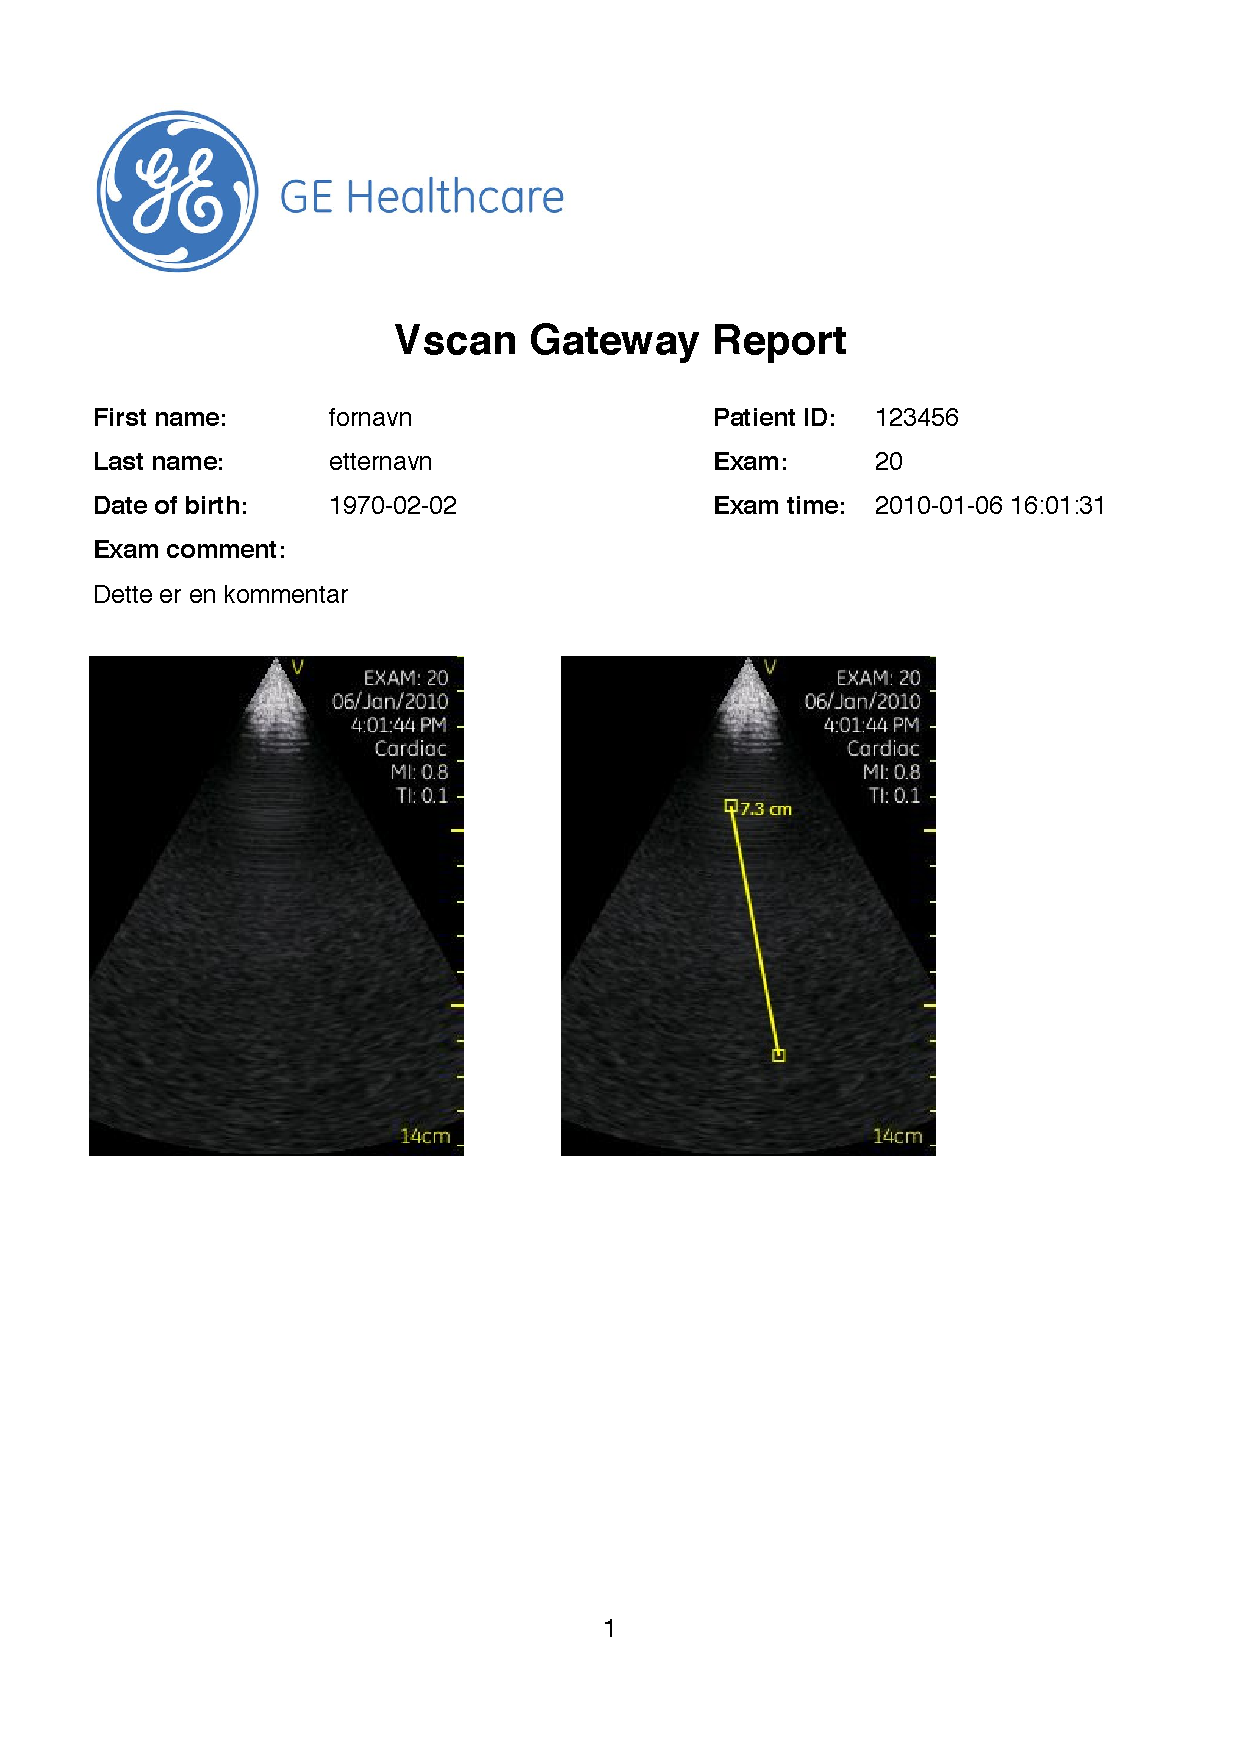
\includepdf[scale=0.72,frame,clip,trim=0cm 2.2cm 0cm 0cm,pages={1},pagecommand={}]{img/exampleGatewayreport1.pdf}


\section{Example report: Backup service}
\label{dummyServiceReport}

This is an example report generated by the backup service.


\includepdf[scale=0.72,frame,clip,trim=0cm 2.2cm 0cm 0cm,pages={1-4},pagecommand={}]{img/example_examination.pdf}
\section{Example of weekly report}
\label{weekly_rep}

This is an example of a typical weekly report. These reports served as a tool for insight for both the customer and the project supervisor.

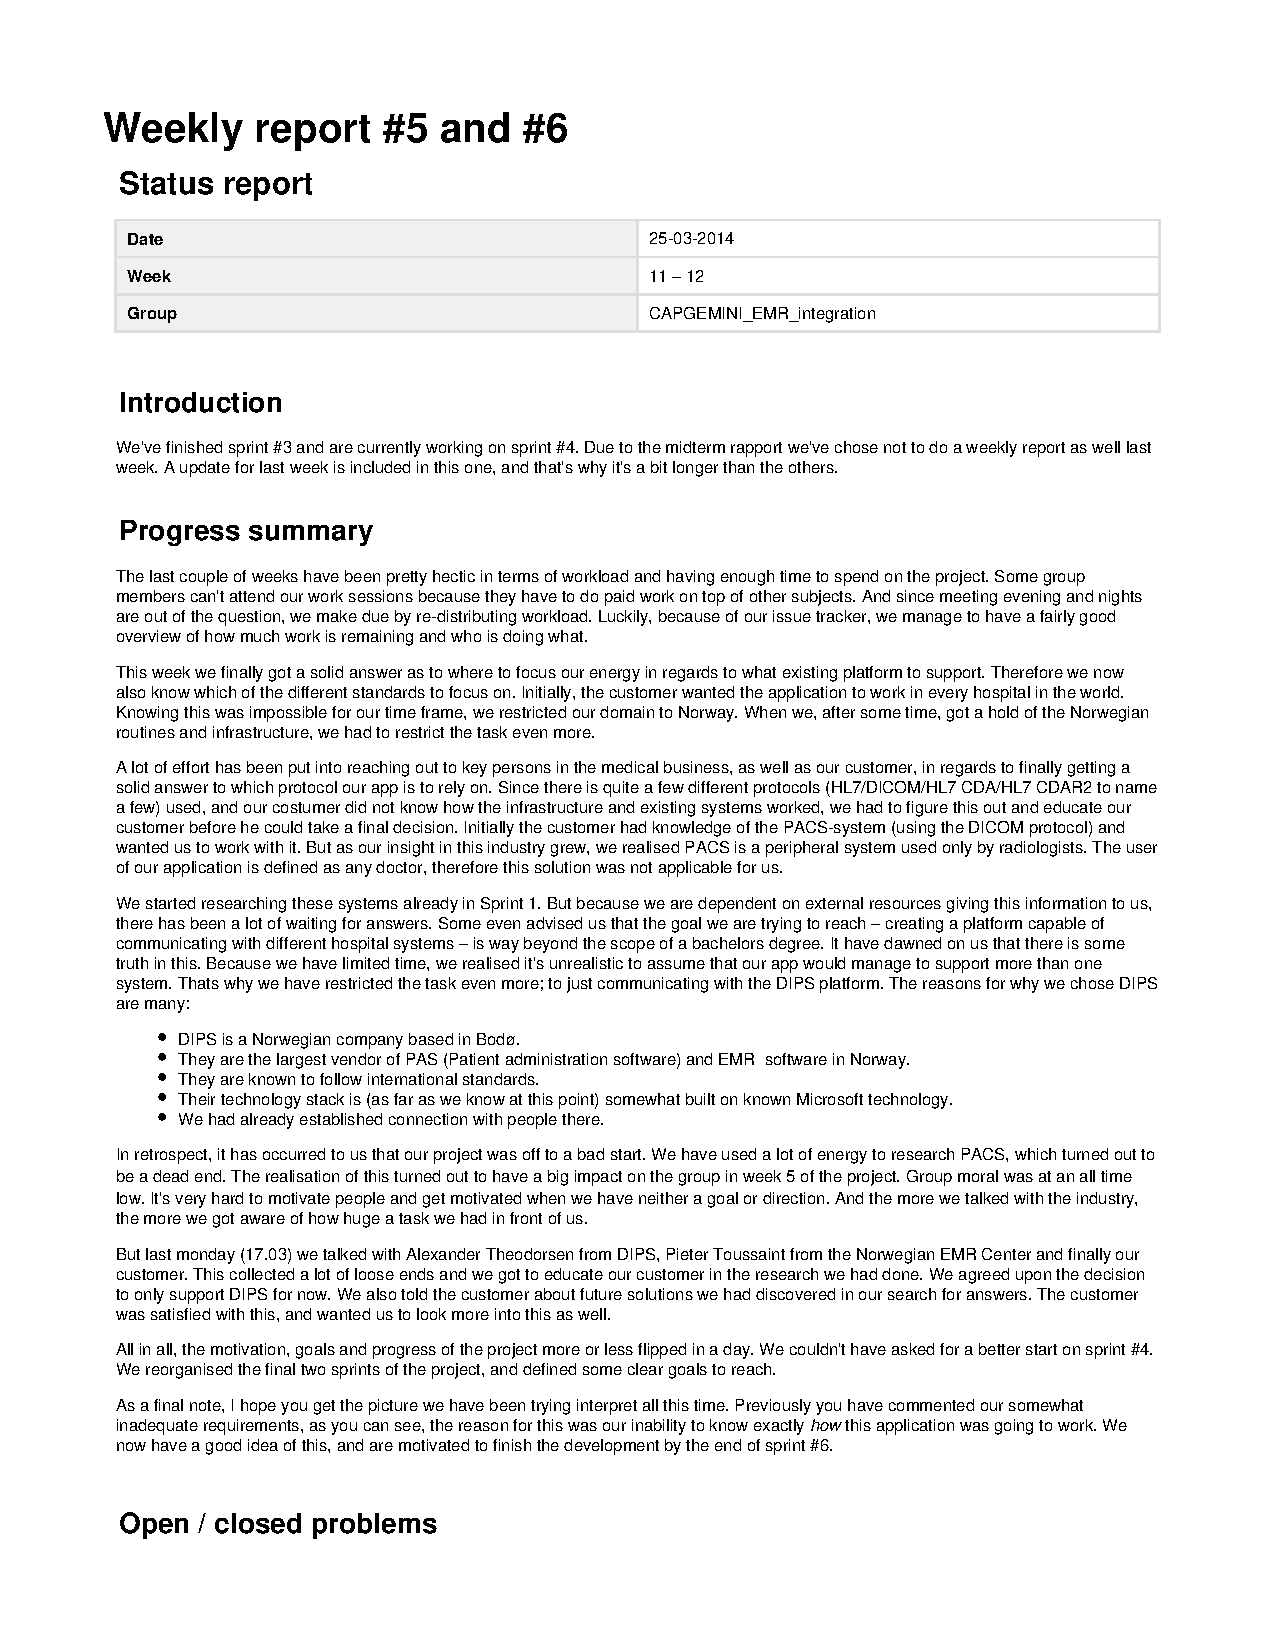
\includepdf[scale=0.72,frame,clip,trim=0cm 1.90cm 0cm 0cm,pages={1-2},pagecommand={}]{img/weekly/weekly5and6.pdf}
\section{User Manual}
\label{usermanual}
The following document is the user manual for the application.


\newpage
\begin{center}
    \vspace*{1cm}
    
    \huge{Gateway 2.0 - User's Manual}
    
    \vspace{2cm}
    \normalsize
    A quick guide for navigating and using \\the Gateway 2.0 application for Android.
    
    
    \vfill
    
    
    \normalsize
    {Rikard Eide\\Andreas Røyrvik\\Jens Kristian Espevik\\Joakim Pettersen\\Magnus Lund\\}
    \vspace{0.8cm}
    NTNU: Norwegian University of Science and Technology\\
    \vspace{0.8cm}
    \today
    \vspace{0.8cm}
    
\end{center}
\newpage

\subsection*{Preface}
This application was designed to be a link between the Vscan application and hospital servers. The application can be started in three different modes; (1) go directly to the "Not yet uploaded"-view, (2) identify the patient and return to Vscan, or (3) start normally with the workflow described in the rest of this guide.

\newpage
\subsection*{Login}
This is the first view you will see when you start the application. From here you can either log into the application or access the settings. To log in to the application, enter your personal username and password and hit the login button. This will start a new session, saving your credentials for up to 10 minutes after the last time you did something in the application. To log out before the 10 minutes has passed, navigate to the "Not yet uploaded" screen and press log out.
If the password you use to log in has changed since the last time the application was started, you will be asked to enter the password you used the last time to change the database password to match the new one.

\begin{figure}[H]
\centering
    \begin{subfigure}[b]{0.49\textwidth}
        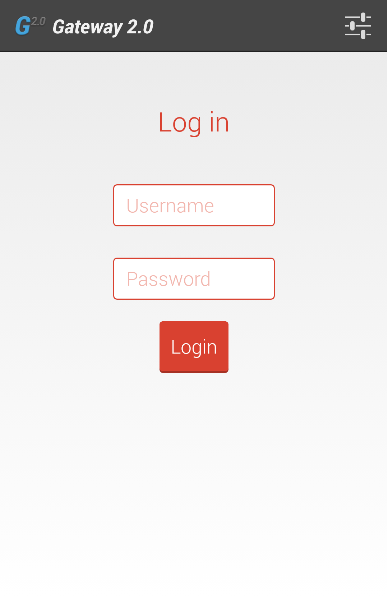
\includegraphics[width=\textwidth]{img/interface/1-Login.png}
        \caption*{Login View}
        \label{fig:01login}
    \end{subfigure}
    \begin{subfigure}[b]{0.49\textwidth}
        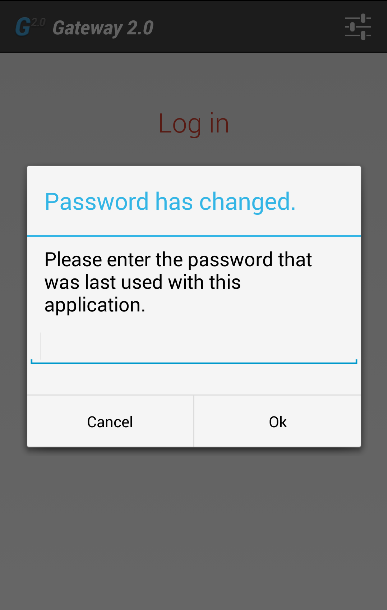
\includegraphics[width=\textwidth]{img/interface/14-DatabasePassword.png}
        \caption*{Password has changed}
        \label{fig:14dbpassword}
    \end{subfigure}
\end{figure}

\newpage
\subsection*{Identify}
In this view you will first have to choose to either identify the patient manually, by typing the SSN, or automatically by scanning a QR code or barcode. To use the automatic feature you will have to install the "Barcode Scanner" application. If you choose automatic mode without having the appropriate application installed, you will be met with a dialog asking you to install it.

When you have chosen the preferred identifying method, you will see a new view with a number input field, where you can enter the SSN or check the SSN gathered from the QR scanner. Pressing the "OK" button will get patient information from the hospital servers and start a new examination.

\begin{figure}[H]
\centering
    \begin{subfigure}[b]{0.49\textwidth}
        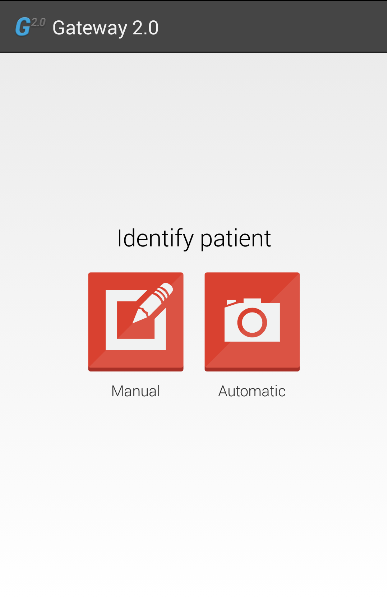
\includegraphics[width=\textwidth]{img/interface/2-Identify1.png}
        \caption*{Choose Identify Method}
        \label{fig:02identify}
    \end{subfigure}
    \begin{subfigure}[b]{0.49\textwidth}
        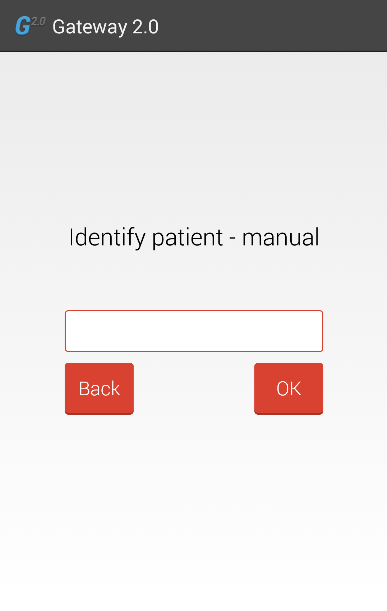
\includegraphics[width=\textwidth]{img/interface/3-Identify2.png}
        \caption*{Enter Patient SSN}
        \label{fig:03identify}
    \end{subfigure}
\end{figure}

\newpage
\subsection*{Examination}
This view will show all available information about the current examination. A small icon next to the SSN will indicate whether the SSN is validated or not. Clicking the SSN, or the small pen icon, will redirect you to the identify view where you can change or validate the SSN. To add an examination comment, click the examination comment text, or the small pen icon in front of it.

Pressing the “View images” button will bring up the commenting view covered in the next section. Two lines of text below the button will tell you the number of images both with and without comment. When you are done with the examination, you can click the “Review and Upload” button, which will bring you to the "Review and Upload" view.

\begin{figure}[H]
\centering
    \begin{subfigure}[b]{0.49\textwidth}
        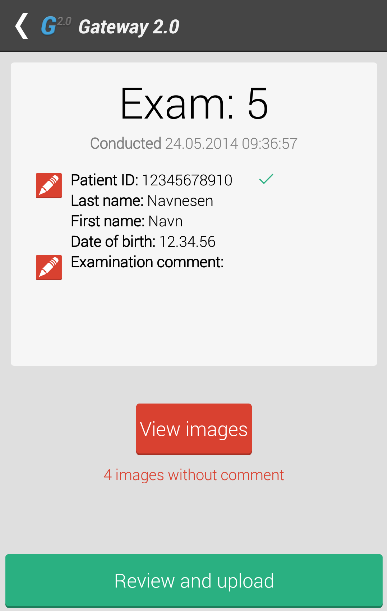
\includegraphics[width=\textwidth]{img/interface/4-Examination.png}
        \caption*{Examination View}
        \label{fig:04examination}
    \end{subfigure}
    \begin{subfigure}[b]{0.49\textwidth}
        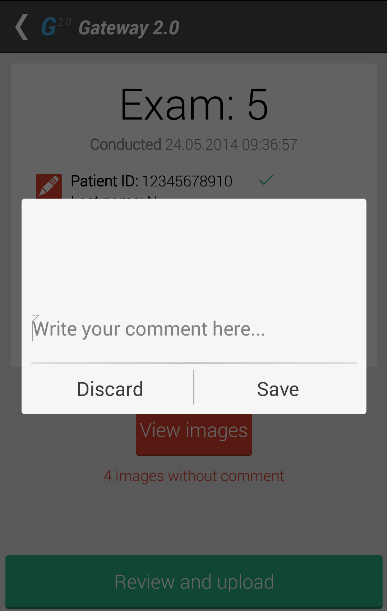
\includegraphics[width=\textwidth]{img/interface/5-ExaminationComment.png}
        \caption*{Examination Comment}
        \label{fig:05examinationcomment}
    \end{subfigure}
\end{figure}

\newpage
\subsection*{Commenting}
In this view you can swipe through all the images in the current examination. At the bottom there are two buttons; the trashcan, which will remove the image from the examination, as well as the commenting button, which will bring up a dialog where you can add a comment to the image. When you are done commenting, you can press the “close” button to return to the "Examination" view. Using the hardware back button will discard all changes and return to the "Examination" view.

\begin{figure}[H]
\centering
    \begin{subfigure}[b]{0.49\textwidth}
        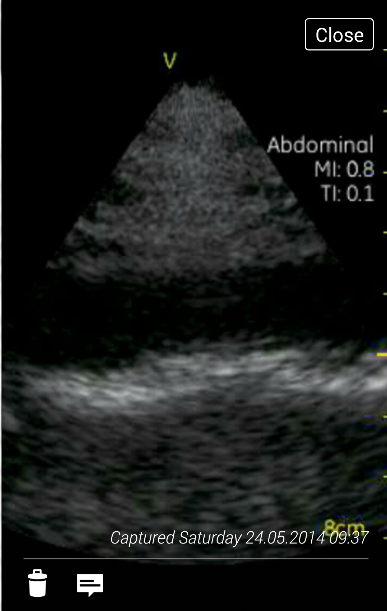
\includegraphics[width=\textwidth]{img/interface/6-ViewImage.png}
        \caption*{Full screen View}
        \label{fig:06viewimage}
    \end{subfigure}
    \begin{subfigure}[b]{0.49\textwidth}
        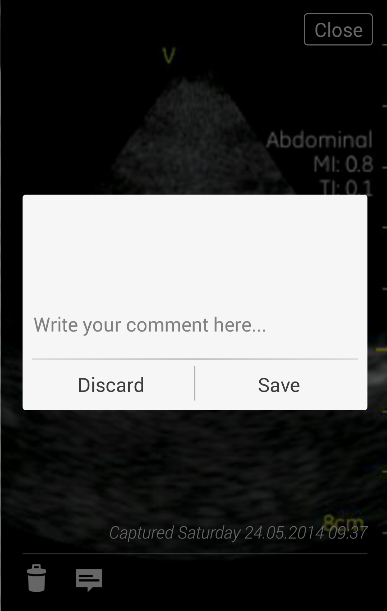
\includegraphics[width=\textwidth]{img/interface/7-ViewImageComment.png}
        \caption*{Enter Image Comment}
        \label{fig:07viewimagecomment}
    \end{subfigure}
\end{figure}

\newpage
\subsection*{Review and Upload}
This view will force you to look through all the information in the examination before uploading it to the hospital servers. When you scroll down to the bottom, there are two buttons: an edit that button will return you to the examination view, and an upload button that will upload the examination. If the upload is successful, the examination will be removed from the local database and you will be redirected to the not yet uploaded view.

If for some reason the upload fails to complete you can press “edit” to go back to the examination view, then the back button to go to the not yet uploaded view. The current examination will remain in the local database, and you can find it in the not yet uploaded view to upload it when you have a connection to the hospital servers.

\begin{figure}[H]
\centering
    \begin{subfigure}[b]{0.49\textwidth}
        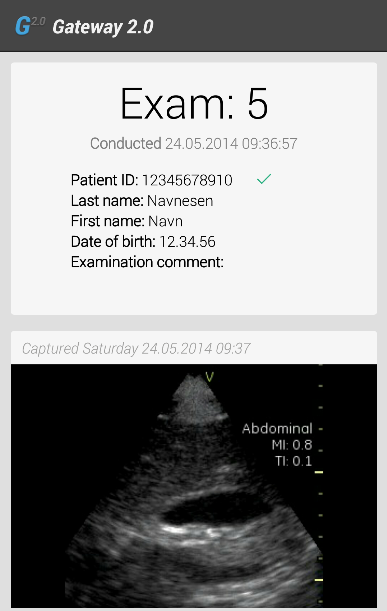
\includegraphics[width=\textwidth]{img/interface/8-ReviewAndUpload.png}
        \caption*{Top of the view}
        \label{fig:08review}
    \end{subfigure}
    \begin{subfigure}[b]{0.49\textwidth}
        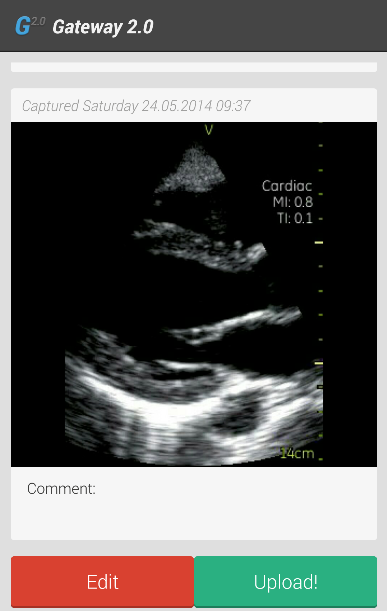
\includegraphics[width=\textwidth]{img/interface/9-ReviewAndUploadEnd.png}
        \caption*{Buttons at the end}
        \label{fig:09reviewend}
    \end{subfigure}
\end{figure}

\newpage
\subsection*{Not yet uploaded}
A list of all saved examinations will be listed in this view. This view is also the only view where you will have the option to log out of the application. Clicking one of the examinations will bring up a dialog where you can choose to either delete the examination from the database or open it in the examination view by choosing edit.

\begin{figure}[H]
\centering
    \begin{subfigure}[b]{0.49\textwidth}
        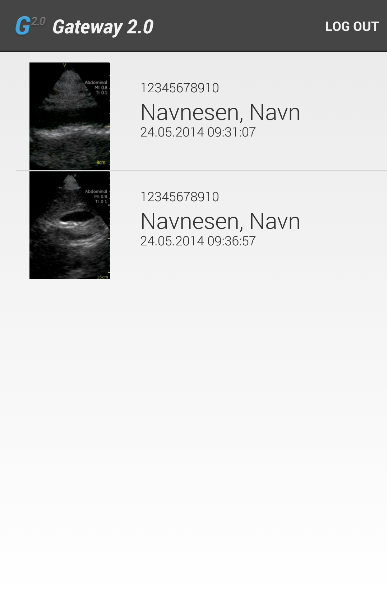
\includegraphics[width=\textwidth]{img/interface/10-NotYetUploaded.png}
        \caption*{Not Yet Uploaded View}
        \label{fig:11notyetuploaded}
    \end{subfigure}
    \begin{subfigure}[b]{0.49\textwidth}
        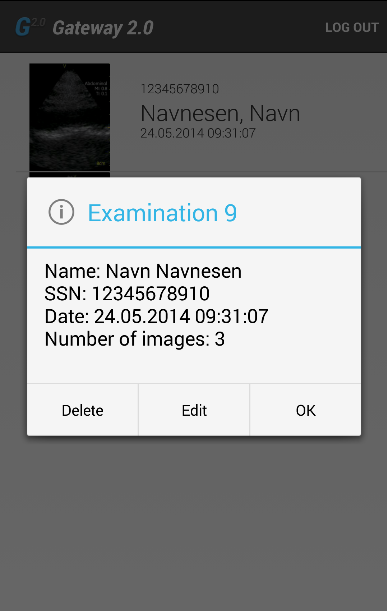
\includegraphics[width=\textwidth]{img/interface/11-DeleteExamination.png}
        \caption*{Examination Choices}
        \label{fig:12delete}
    \end{subfigure}
\end{figure}

\begin{figure}[H]
\centering
    \begin{subfigure}[b]{0.49\textwidth}
        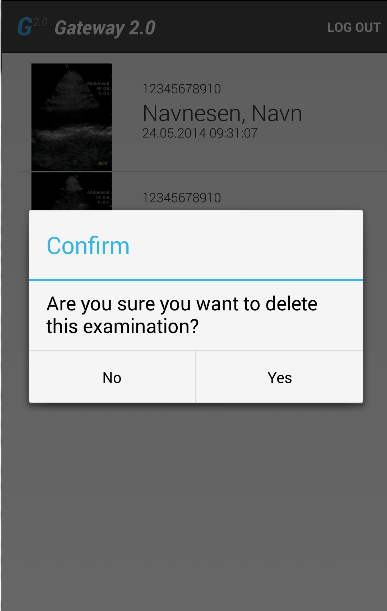
\includegraphics[width=\textwidth]{img/interface/12-ConfirmDeleteExamination.png}
        \caption*{Confirm deletion of examination}
        \label{fig:12confirmdelete}
    \end{subfigure}
    \begin{subfigure}[b]{0.49\textwidth}
        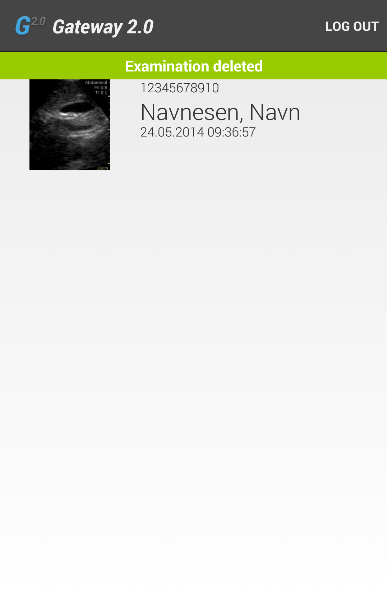
\includegraphics[width=\textwidth]{img/interface/13-NotYetUploadedPostDelete.png}
        \caption*{Not Yet Uploaded view after deletion}
        \label{fig:13notyetuploadedpost}
    \end{subfigure}
\end{figure}

\newpage
\subsection*{Settings}
Then only thing you can do in this view without the technical password is to change the language. More information regarding the other options in this view is explained in the technical manual.

\begin{figure}[H]
\centering
    \begin{subfigure}[b]{0.49\textwidth}
        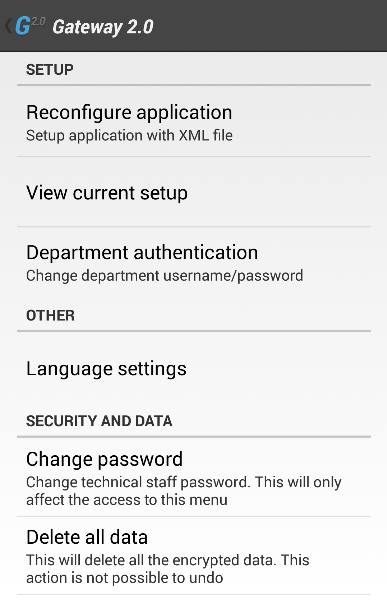
\includegraphics[width=\textwidth]{img/interface/15-Settings.png}
        \caption*{Settings View}
        \label{fig:15settings}
    \end{subfigure}
    \begin{subfigure}[b]{0.49\textwidth}
        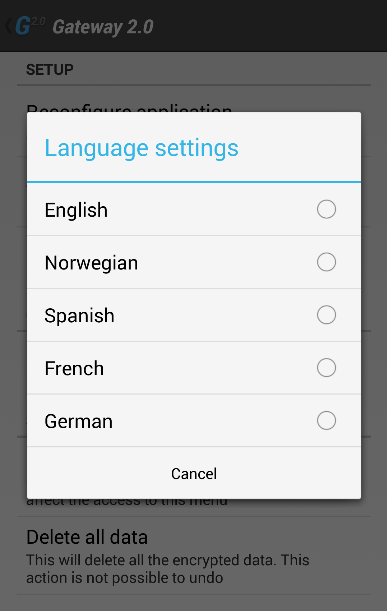
\includegraphics[width=\textwidth]{img/interface/16-Language.png}
        \caption*{Language Select}
        \label{fig:16language}
    \end{subfigure}
\end{figure}

\newpage
\subsection*{Troubleshooting}

\begin{itemize}
\item When the app starts it asks for the tech password.
    \begin{itemize}
	\item The app is not set up properly, contact technical support or refer to the technical manual
	\end{itemize}

\item I have the correct SSN, but the Identify Patient View says it is invalid
    \begin{itemize}
    \item The invalid ID error can be caused by two things; either the entered ID is wrong, or the service is unavailable. Check the SSN one more time, and recheck your network connection.
    \end{itemize}

\item Review and Upload button can not be clicked
    \begin{itemize}
	\item The ID hasn't been validated, click the current ID to validate.
	\end{itemize}
    
\end{itemize}
\section{Technical User Guide}
\label{techmanual}

This guide will handle the initial setup of the application as well as the creation of the settings file. As the settings file is needed for the initial setup, this will be covered first.

\subsection{The settings file}
This is the general layout of the settings file:

\lstset{language=XML}
\begin{lstlisting}[caption={settings.xml}, label={lst:settingsxml}]
<settings>
<systemPackage>
    <aidlLocation>
    <servicePath>
</systemPackage>
<authentication>
    <authenticationProtocol>
    <authenticationServerAddress>
    <authenticationServerPort>
    <LDAPuserID>
    <LDAPOU>
    <LDAPDC>
</authentication>
</settings>
\end{lstlisting}

The \textit{systemPackage} category handles service communication. \textit{aidlLocation} should point to the package where the \textit{.aidl} file is located, \textit{org.royrvik.emrservice} by default. The \textit{servicePath} field should give the full path to the service. If the service is called EMRService and is located in the \textit{org.royrvik.emrservice} package, this field would be \textit{org.royrvik.emrservice.EMRService}.

The second category handles communication with authentication servers. The first field, \textit{authenticationProtocol}, tells the system which authentication system to use, currently being either LDAP or LDAPS. The next two fields are server address and server port, followed by your servers OU and DC. 

As an example, here is a settings file pointing at a service called EMRService in the org.royrvik.emrservice package. The \textit{.aidl} file is in the same package, and the authentication is set to use the NTNU's LDAPS servers.

\begin{lstlisting}[caption={An example settings file}, label={lst:examplesettings}]

<settings>
    <systemPackage>
        <aidlLocation>org.royrvik.emrservice</aidlLocation>
        <servicePath>org.royrvik.emrservice.EMRService
        </servicePath>
    </systemPackage>
    <authentication>
        <authenticationProtocol>ldaps</authenticationProtocol>
        <authenticationServerAddress>
            at.ntnu.no
        </authenticationServerAddress>
        <authenticationServerPort>636
        </authenticationServerPort>
        <LDAPuserID>uid</LDAPuserID>
        <LDAPOU>people</LDAPOU>
        <LDAPDC>ntnu.no</LDAPDC>
    </authentication>
</settings>
\end{lstlisting}
\subsection{Initial setup}
When the application is first launched, it will detect that it is not set up properly, and redirect the user to the technical setup. The first step of this setup is choosing a tech user password. This password is used later to reconfigure the application or display the current settings. The next step will prompt the user for a path to the settings file. This can be both a local file and a file on a web-server. Clicking \textit{Get settings} will then make the application read and validate the settings. If the setup was successful the finish button will exit the application, and it is now ready for use.
\section{Service Development Guide}
\label{devmanual}

This guide will handle the steps necessary to start developing custom services for the EMR Application.

To get started, create a new android project with a package named \textit{org.royrvik.emrservice}. Create a new file in the package and name it \textit{EMRRemoteInterface.aidl}. It is crucial that these exact package- and file names are used. Add the following code to the file:
\newline


\begin{lstlisting}[caption={EMRRemoteInterface.aidl}, label={lst:emrremoteinterface}]
// EMRRemoteInterface.aidl
package org.royrvik.emrservice;

interface EMRRemoteInterface {
    List<String> getPatientData(in String ssn, in String username, in String password);
    List<String> upload(in List<String> examinationData, in List<String> imagePaths, in List<String> notes, in String username, in String password);
}
\end{lstlisting}

\smallskip

Compile the newly created .aidl file, this will create a new Java interface in \textit{gen/org.royrvik.emrservice} within the project. It might be necessary to reopen the IDE for this file to appear. The setup of the AIDL is now complete.

To create the service itself, make a new class extending android.app.Service. In the service class, create a new \textit{private final EMRRemoteInterface.Stub} variable and initiate it with \textit{EMRRemoteInterface.Stub}. In the following example, the variable is named \textit{service}. The IDE should now complain that there are unimplemented methods in the Stub interface, let it auto implement the two methods \textit{getPatientData()} and \textit{upload()}. Now make the service's \textit{onBind()} method return the EMRRemoteInterface.Stub variable instead of the default \textit{null}. To make the service accessible from other projects and add \textit{android:exported="true"} to the \textit{service} tag in the \textit{AndroidManifest.xml}. From here, simply replace \textit{return null} in both implemented methods from the interface with custom code for the required environment. Following is an example implementation of the service and the manifest as well as a table of expected input/output.


\begin{lstlisting}[caption={ExampleService.java}, label={lst:exampleservice}]
package org.royrvik.emrservice;

import android.app.Service;
import android.content.Intent;
import android.os.IBinder;
import android.os.RemoteException;
import java.util.List;

public class ExampleService extends Service {
    public IBinder onBind(Intent intent) {
        return service;
    }

    private final EMRRemoteInterface.Stub service = new EMRRemoteInterface.Stub() {

        @Override
        public List<String> getPatientData(String ssn, String username, String password) throws RemoteException {
            //YOUR CODE HERE
            return null;
        }

        @Override
        public List<String> upload(List<String> examinationData, List<String> imagePaths, List<String> notes, String username, String password) throws RemoteException {
            //YOUR CODE HERE
            return null;
        }
    };
}
\end{lstlisting}



\newpage

\lstset{language=XML}
\begin{lstlisting}[caption={AndroidManifest.xml}, label={lst:manifest}]
<?xml version="1.0" encoding="utf-8"?>
<manifest xmlns:android="http://schemas.android.com/apk/res/android"
          package="org.royrvik.emrservice">
    <uses-sdk android:minSdkVersion="17"/>
    <application android:icon="@drawable/icon" android:label="@string/app_name">
        <service android:name=".ExampleService" android:exported="true"/> <!-- Important
    </application>
</manifest>
\end{lstlisting}

\newpage

\noindent Expected service input/output:
\newline
\textit{getPatientData()}
\begin{itemize}
\item Input:
    \begin{itemize}
    \item String ssn
    \item String username
    \item String password
    \end{itemize}
\item Output:
    \begin{itemize}
    \item List$<$String$>$
        \begin{itemize}
        \item 0 - int didWork
        \item 1 - String ssn
        \item 2 - String firstName
        \item 3 - String lastName
        \item 4 - String errorMesage
        \end{itemize}
    \end{itemize}
\end{itemize}
\newpage
\textit{upload()}
\begin{itemize}
\item Input:
    \begin{itemize}
    \item List$<$String$>$
        \begin{itemize}
        \item 0 - String ssn
        \item 1 - String firstName
        \item 2 - String lastName
        \item 3 - String examNumber
        \item 4 - String examTime
        \item 5 - String examComment
        \end{itemize}
    \item List$<$String$>$ imagePaths
    \item List$<$String$>$ notes
    \item String username
    \item String password
    \end{itemize}

\item Output:
    \begin{itemize}
    \item List$<$String$>$
        \begin{itemize}
        \item 0 - int didWork
        \item 1 - String errorMessage
        \end{itemize}
    \end{itemize}
\end{itemize}
\section{Contacts}
\label{contacts}
While doing our research we have been in contact with several people in numerous areas of the medical sector, both in IT and other areas. Bellow is a list of essential people which has helped the group in its research.

\begin{table}[H]
\renewcommand{\arraystretch}{1.2}
\begin{tabular}{|p{4cm}|p{9cm}|}
\hline

Heidi Thorstensen & \begin{tabular}[c]{@{}l@{}}
Responsible for privacy and information security at\\ Oslo University Hospital
\end{tabular} \\ \hline

Bjørn Næss & \begin{tabular}[c]{@{}l@{}}
Product owner at DIPS ASA
\end{tabular} \\ \hline

Roald Bergstrøm & \begin{tabular}[c]{@{}l@{}}
Senior Advisor at KITH
\end{tabular} \\ \hline

Mikal Reed & \begin{tabular}[c]{@{}l@{}}
Project manager and developer at Konik AS
\end{tabular} \\ \hline

Ole Christian Mjølstad & \begin{tabular}[c]{@{}l@{}}
Phd, Department of Circulation and Medical Imaging
\end{tabular} \\ \hline

Ragnvald Otterlei & \begin{tabular}[c]{@{}l@{}}
Posicom AS - Provider of hospital multimedia\\solutions
\end{tabular} \\ \hline

Alexander Theodorsen & \begin{tabular}[c]{@{}l@{}}
Section manager at DIPS ASA
\end{tabular} \\ \hline

Pieter Jelle Toussaint & \begin{tabular}[c]{@{}l@{}}
Professor IDI NTNU, Deputy at the Norwegian \\Research Centre for Electronic Patient Record
\end{tabular} \\ \hline

Øystein Nytrø & \begin{tabular}[c]{@{}l@{}}
Associate Professor IDI NTNU
\end{tabular} \\ \hline

%%%%%%%%%%%%%%%%%%

Svein Pettersen & \begin{tabular}[c]{@{}l@{}}
Product owner at DIPS ASA
\end{tabular} \\ \hline

Line Andreassen Sæle & \begin{tabular}[c]{@{}l@{}}
System architect at Helse Vest IKT
\end{tabular} \\ \hline

Arne Martin Eide & \begin{tabular}[c]{@{}l@{}}
Cardiologist at Kiel University Hospital
\end{tabular} \\ \hline

Tor Erling Bjørstad & \begin{tabular}[c]{@{}l@{}}
Phd, Senior consultant at Mnemonic
\end{tabular} \\ \hline

Håvard Roterud & \begin{tabular}[c]{@{}l@{}}
Health informatician at Radiologisk IT,\\ Oslo University Hospital
\end{tabular} \\ \hline

Tore Dundas & \begin{tabular}[c]{@{}l@{}}
Product line owner at DIPS ASA
\end{tabular} \\ \hline

Per Olav Skjesol & \begin{tabular}[c]{@{}l@{}}
Programmanager Helse Midt-Norge IT
\end{tabular} \\ \hline

Marit Østrem Ditlevsen & \begin{tabular}[c]{@{}l@{}}
Developer at DIPS ASA
\end{tabular} \\ \hline

Richard Husevåg & \begin{tabular}[c]{@{}l@{}}
Project manager and consultant at Konik AS
\end{tabular} \\ \hline

Øyvind Aassve & \begin{tabular}[c]{@{}l@{}}
Enterprise Architect at Oslo University Hospital
\end{tabular} \\ \hline

Yngve Hals Nyheim & \begin{tabular}[c]{@{}l@{}}
Development manager at DIPS ASA
\end{tabular} \\ \hline

Lars-Gunnar Hartveit & \begin{tabular}[c]{@{}l@{}}
Special consultant Helse Vest IKT
\end{tabular} \\ \hline

\end{tabular}
\end{table}
\section{BizTalk}
\label{biztalk}

When the group first started planning the implementation, the idea was to have a package system to handle the different EMR systems and to have a centralized server with all the packages stored. The package URL would be stated in the settings and the package would be downloaded to the device, and then work as a parser to decode information received from the EMR server. As the group got more information about how the different systems work today, this idea was scrapped because differences between the different EMRs were too big. The group started leaning towards using Android services instead.

\subsection{DIPS HL7Connector}
This new information resulted in a redesign of the functionality used to communicate with the EMRs. Because of our early decision to create a modular architecture, it was possible for us to keep the code we had already written, we only needed to change the approach for how to implement the server communication.

This required us to set up a development environment on a server, as they were only able to whitelist one IP address for us to access the server through. BizTalk natively only allows for implementation through C\#, which required the group to invest a lot of time in research in learning to program in C\#, as well as understanding concept of BizTalk.

The group worked in parallel to both develop the C\# application as well as figuring out how to run a C\# application in Android. It was concluded that the service could be created using Xamarin \cite{xamarin}, but implementational issues with the BizTalk server hindered the group in completing the service. After first debugging the issue together with a Konik consultant as well as developers at Helse Vest IT, we later found out, with help from DIPS developers in Bodø, that the issue resided server side. The empty DIPS mockup server we were given access to had some issues, and was not properly configured to allow for the communication needed.

In addition to this issue, the server did not support any form of uploading of multimedia, which concurrent research at the time revealed to be a problem. These two reasons made us scrap the DIPS service, and go for the simple backup solution.
\section{Security on smart devices}
\label{smartSecurity}

The following section contains some examples on how vulnerable to attacks todays smart devices might be. 

\subsection{Smart devices}
Recently there has been an increase in research regarding the exploitation of so called side-channels on smart phones. In a larger context these channels conclude only some part of the whole attack surface, but by exemplifying this we might give the customer an idea of the wide array of possible threats. As Spreitzer describes in a recent paper \cite{2014arXiv1405.3760S}, these sensors poses a serious threat to the user's privacy and security. Side channels represent unintended information leakage during the operation of a device and potentially allow attackers to recover secret information. Spreitzer and others illustrates how one only by monitoring the built in sensors can measure variations in movement, acceleration, sound or even light intensity and successfully extract sensitive data like keystrokes or even RSA Keys \cite{cryptoeprint:2013:857}. These exploits would bypass software security layers like authentication and encryption, because they rely solely on physical factors.

\subsubsection{Memory}
Another problem we came across was how to handle in-memory data. Android is built on Java and the Dalvik Virtual Machine, where memory management is abstracted from the programmer. Instead it uses a Garbage Collector (GC) to reallocate memory that is no longer being used.
 
Through habits obtained from consumer products users expect a high degree of availability from modern mobile devices. In order to achieve this availability the devices are almost never powered off, and use several techniques like hibernation and sleep modes to preserve battery while keeping the device on. From a technical perspective this also results in keeping the main memory intact. Combined with the portability of mobile devices, this introduces several problems when managing sensitive data: encrypting stored data is no longer enough, as the main memory now is part of the attack surface. We fear the scenario where an attacker would just grab a device and walk away. As mentioned below, encrypting main memory (RAM) does not serve any real purpose, and it would put a lot of constraints on the performance of the device.
 
We found several techniques that makes in-memory data vulnerable as long as the attacker has physical access to the device. The Norwegian developed Inception tool \cite{inception} does exactly this. By exploiting I  EEE 1394 SBP-2 DMA, the software tool claims to unlock and escalate privileges to administrator/root on almost any powered-on machine you have physical access to. It does this by first gaining full read/write access to main memory through the DMA of a physical port. Then it searches the available memory pages, looking for the operating system's password authentication modules. When found, it modifies the code to allow any password. This works as long as the device is powered on, and the physical Direct Memory Access (DMA) compatible I/O ports on the device are enabled. Does this apply to the USB interface? While the lowest-level USB driver that talks to the root hub does DMA, we have yet to find out whether or not this exploit is possible via the USB interface (which is found on the Vscan), but it is not unthinkable. Another entrance for this exploit could be the SD card interface, while we have not researched this further.
 
Another, more advanced attack, that only requires physical access to the device is the \emph{Cold Boot Attack}. The attack is described in a paper by researches from Princeton University \cite{Halderman08leastwe}. This also exploits the data that resides in main-memory, but in a slightly different way. By cutting power to the device and cooling the RAM chip, the bits that reside in RAM fade away slowly. When this is done, one could remove the chip and read it via another device, or boot the device from an external source and copying the contents. This way disk encryption could also be broken because the encryption keys would reside in RAM as long as the device was powered on before the attack begun. Both these examples concludes in the fact that:

\begin{quote} 
\textit{Sensitive data in memory + physical access = major vulnerability}
\end{quote}

\subsection{Prevention}
In Real-Time Computing, making economical allocation of resources in scalable systems is an important problem. This problem can be solved with a programming style here where one is always concerned with the allocation and deallocation of resources. By manually deallocating in-memory data, you put less constrains on the GC and it gives you better control over what application data actually exists in the memory at a given time. A similar technique could be adapted in our case, in order to keep the exposure window of in-memory sensitive data to a minimum. This would have to be decided early in design phase, and is probably really expensive and time consuming to both develop and test.
\section{Package Diagram}
\label{classdiagram}

\begin{figure}[H]
\centering
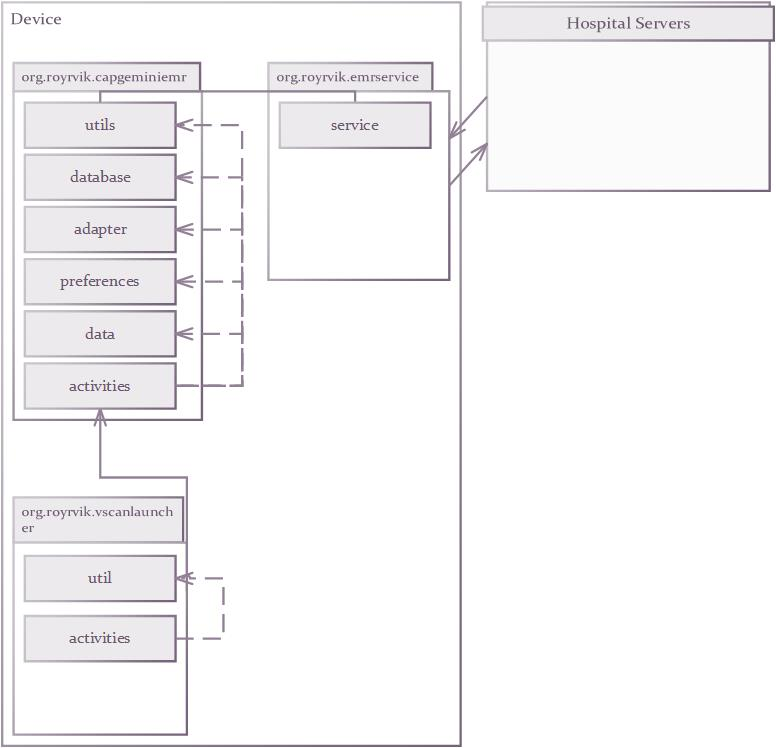
\includegraphics[scale=0.7]{img/classdiagram.jpg}
\caption{Package Diagram}
\label{fig:packagediagram}
\end{figure}
\end{appendices}

\end{document}